\documentclass[12pt,twoside,reqno]{article}
%\documentclass[11pt,twoside,reqno]{article}


\usepackage{ngerman}
\usepackage{amsmath}
\usepackage{amsbsy,wasysym}
\usepackage{fleqn}
\usepackage{latexsym}
\usepackage{epsfig}
\usepackage{amssymb}
\usepackage[version=3]{mhchem}

%\usepackage{mythm}
%\usepackage{amsthm}

\usepackage[amsmath,amsthm,thmmarks]{ntheorem}
\usepackage{textpos}
\usepackage{enumerate}

\usepackage{float}
% \usepackage[latin1]{inputenc}
\usepackage[utf8]{inputenc}
\usepackage{t1enc}
\usepackage{tikz}
\usepackage{times}
\usepackage{mathptmx}
\usepackage{stmaryrd}
%\usepackage[colorlinks=false,
\usepackage[colorlinks=true,
            pdftitle={Lectures},
            pdfauthor={Christian Wieners},
            pdfpagemode={UseOutlines},pdfstartview={Fit},
            linkcolor=blue,urlcolor=blue,
%            linkcolor=black,urlcolor=black,
            pdfsubject={Numerik III}]{hyperref}

%\renewcommand{\rmdefault}{phv}

\textwidth 151mm
\textheight246mm
\topmargin-20mm
\evensidemargin0mm
\oddsidemargin8.0mm
\parindent=0pt
\parskip=3pt plus 1pt
%\normalparindent=0pt
\mathindent = 15mm

\newcommand{\mbf}[1]{\mathbf #1}  % fette Griechen
\newcommand{\cbf}[1]{{\mbox{\boldmath${\mathcal #1}$}}}  % fett Cal

\restylefloat{figure}
\restylefloat{table}

\newcommand\GL{\text{GL}}
\newcommand\Real{\mathbb{R}}
\newcommand\Natural{\mathbb{N}}
\newcommand\Complex{\mathbb{C}}
\newcommand\Integer{\mathbb{N}}
\newcommand\Polynom{\mathbb{P}}
\newcommand\TensorElem{\mathbb{Q}}

\newcommand{\oh}{\frac{1}{2}} % oh -> one half

\newcommand\frachalf{\mbox{\large $\frac12$}}
%\newcommand\sL{\mathrm{sl}}
\newcommand\SL{\mathrm{SL}}
\newcommand\bsl{\mathbf{sl}}
\newcommand\bSL{\mathbf{SL}}

\renewcommand{\d}{\,\mathrm{d}}
\newcommand{\dx}{\,\mathrm{d}x}
\newcommand{\dy}{\,\mathrm{d}y}
\newcommand{\da}{\,\mathrm{d}a}
\newcommand{\dt}{\,\mathrm{d}t}

\newcommand{\Nodes}{\mathcal{V}_h}
\newcommand{\Faces}{\mathcal{E}_h}
\newcommand{\FacesInterior}{\Faces^\text{int}}

\newcommand{\TriangulationLetter}{\mathcal{T}}
\newcommand{\Triangulation}{\TriangulationLetter_h}

\newcommand{\FEMLinear}{\mathcal{S}_h^1}

\newcommand{\term}[1]{\emph{#1}}


\newcommand\sym{\operatorname*{sym}}
\newcommand\supp{\operatorname*{supp}}
\newcommand\Span{\operatorname*{span}}
\newcommand\Spur{\operatorname*{Spur}}
\newcommand\rank{\operatorname*{rank}}
\newcommand\interior{\operatorname*{int}}
\newcommand\rang{\operatorname*{rang}}
\newcommand\curl{\operatorname{curl}}
\newcommand\const{\operatorname*{const}}
\newcommand\grad{\operatorname*{grad}}
\newcommand\Hess{\operatorname{Hess}}
\newcommand\dev{\operatorname*{dev}}
\newcommand\Kern{\operatorname*{Kern}}
\newcommand\diag{\operatorname*{diag}}
\newcommand\Diag{\operatorname*{diag}}
\newcommand\tridiag{\operatorname*{tridiag}}
\newcommand\Lower{\operatorname*{lower}}
\newcommand\Upper{\operatorname*{upper}}
\newcommand\dist{\operatorname*{dist}}
\newcommand\tr{\operatorname*{trace}}
\newcommand\dom{\operatorname*{dom}}
\renewcommand\div{\operatorname{div}}
\renewcommand\Im{\operatorname*{Im}}
\newcommand\dest{\operatorname{dest}}
\newcommand\id{\operatorname{id}}
\newcommand\polar{\operatorname{polar}}
% \renewcommand\inf{\operatorname*{\phantom{p}\!{\rm inf}\!\phantom{p}}}
\newcommand\EN{|\!|\!|}
\newcommand\call[1]{{\sc #1}\index{#1}}
\newcommand\meas{\operatorname{meas}}

\newcommand\conv{\operatorname*{conv}}
\newcommand\sgn{\operatorname*{sgn}}
\renewcommand\Re{\operatorname*{Re}}
\newcommand\diam{\operatorname*{diam}}

\newcommand\Epsilon{\mathcal{E}}

\newcommand\Sym{\operatorname{Sym}}
\renewcommand\skew{\operatorname{skew}}
\newcommand\anti{\operatorname{anti}}
\renewcommand\eqsim{\begin{array}{c}\\[-4mm]=\\[-3.2mm] \sim\end{array}}

\def\u#1{\underline{#1}}
\def\b#1{\boldsymbol{#1}}
%\def\b#1{\mathbf{#1}}
\def\m#1{\mathcal{#1}}
%\def\o#1{\overline{#1}}
\def\i{{\mathrm i}}

%�NDERUNG DER GRIECHISCHEN BUCHSTABEN
\mathchardef\bGamma="0100
\mathchardef\bDelta="0101
\mathchardef\bTheta="0102
\mathchardef\bLambda="0103
\mathchardef\bXi="0104
\mathchardef\bPi="0105
\mathchardef\bSigma="0106
\mathchardef\bUpsilon="0107
\mathchardef\bPhi="0108
\mathchardef\bPsi="0109
\mathchardef\bOmega="010A
\renewcommand{\Omega}{\bOmega}
\renewcommand{\Psi}{\bPsi}
\renewcommand{\Phi}{\bPhi}
\renewcommand{\Xi}{\bXi}
\renewcommand{\Gamma}{\bGamma}
\renewcommand{\Upsilon}{\bUpsilon}



% 4th order tensors
\newcommand\bII{{\mathbb{I}}}    % identity
\newcommand\bCC{{\mathbb{C}}}    % consistent tangent
\newcommand\bGG{{\mathbb{G}}}
\newcommand\bPP{{\mathbb{P}}}    % deviatoric projection tensor
\newcommand\Ttt{{_{23} \atop T}} % 2-3 transposition of identity
\newcommand\Ttf{{_{24} \atop T}} % 2-4 transposition of identity
\newcommand\Tot{{_{13} \atop T}} % 1-3 transposition of identity

% matrices
\newcommand\bI{1\!\!1 }
\newcommand\Id{\operatorname*{Id}}
\newcommand\bC{\mathbf{C}}
\newcommand\bD{\mathbf{D}}
\newcommand\bF{\mathbf{F}}
\newcommand\bE{\mathbf{E}}
\newcommand\bH{\mathbf{H}}
\newcommand\bK{\mathbf K}
\newcommand\bM{\mathbf{M}}
\newcommand\bS{\mathbf{S}}
\newcommand\bP{\mathbf{P}}

% vectors
\def\beps{\text{\boldmath$\varepsilon$\unboldmath}}
\def\bphi{{\text{\boldmath$\varphi$\unboldmath}}}
\def\btheta{{\text{\boldmath$\theta$\unboldmath}}}
\def\bfeta{{\text{\boldmath$\eta$\unboldmath}}}
\def\bpsi{{\text{\boldmath$\psi$\unboldmath}}}
\def\brho{{\text{\boldmath$\rho$\unboldmath}}}
\def\bsigma{\text{\boldmath$\sigma$\unboldmath}}
\def\btau{{\text{\boldmath$\tau$\unboldmath}}}
\def\bxi{{\text{\boldmath$\xi$\unboldmath}}}
\def\bkappa{{\text{\boldmath$\kappa$\unboldmath}}}

\def\bLambda{\text{\boldmath$\Lambda$\unboldmath}}
\def\bSigma{\text{\boldmath$\Sigma$\unboldmath}}
\def\bXi{{\text{\boldmath$\Xi$\unboldmath}}}

\def\vecnull{\hbox{\small{\bf 0}}}
\newcommand\Chi{\chi}
\newcommand\hchi{{\hat\chi}}

%%%%%%%%%%%%%%%%%%%%%%%% Styles-Neff

\newcommand{\Dphi}{\nabla\! \mathbf{\varphi}}
\renewcommand{\epsilon}{\varepsilon}
\newcommand{\dS}{\,{\rm dS} }
\newcommand{\dV}{\,{\rm dV} }
%\newcommand{\dom}{\,{\rm d}\omega }
\newcommand{\norm}[1]{\|#1\|}

\newcommand{\Proof}{{\bf Beweis:\;}}
\newcommand{\ann}{{\it Annahme:\;}}

%\newcommand{\Chi}{\raisebox{0.5ex}{\mbox{{\Large $\chi$}}}}
\newcommand{\flow}{\mbox{{\Large $\mathfrak{f}$}}}
\newcommand{\yieldlimit}{\sigma_{\mathrm{y}}}
\newcommand{\ddelta}{\mbox{\tiny $\Delta$}}

\newcommand{\Mprod}[2]{ {\langle #1 ,#2\rangle} }
\newcommand{\skp}[3]{\langle #1,#2\rangle_#3}
%\newcommand{\id}{ {1\!\!\!\:1 } }
%\newcommand{\qed}{\hfill $\blacksquare$\\}
\newcommand{\qeda}{\tag*{$\blacksquare$} }

\newcommand{\lc}{\mathit{l}_c}

\newcommand{\R}{\mathbb{R}}
\newcommand{\N}{\mathbb{N}}
\newcommand{\C}{\mathbb{C}}
\newcommand{\M}{\mathbb{M}}
\newcommand{\D}{\mathbb{D}}
\newcommand{\Z}{\mathbb{Z}}
\renewcommand{\S}{\mathbb{S}}
\renewcommand{\P}{\mathbb{P}}
\newcommand{\sigmad}{\hat{\sigma}}
\newcommand{\ud}{\hat{u}}
\newcommand{\xd}{\hat{x}}
\newcommand{\kappad}{\hat{\kappa}}
\newcommand{\varphid}{\hat{\varphi}}
\newcommand{\Omegad}{\hat{\Omega}}
\newcommand{\omegad}{\hat{\omega}}
\newcommand{\gammad}{\hat{\gamma}}
\newcommand{\Gammad}{\hat{\Gamma}}
\newcommand{\rd}{\hat{r}}
\newcommand{\sigmas}{\tilde{\sigma}}
\newcommand{\us}{\tilde{u}}
\newcommand{\xs}{\tilde{x}}
\newcommand{\kappas}{\tilde{\kappa}}
\newcommand{\varphis}{\tilde{\varphi}}
\newcommand{\Omegas}{\tilde{\Omega}}
\newcommand{\omegas}{\tilde{\omega}}
\newcommand{\gammas}{\tilde{\gamma}}
\newcommand{\Gammas}{\tilde{\Gamma}}
\newcommand{\rs}{\tilde{r}}



\def\ul#1{\underline #1}
\def\dis{\displaystyle}
\def\ul{\underline}

\newenvironment{rcases}{%
  \left.\renewcommand*\lbrace.%
  \begin{cases}}%
{\end{cases}\right\rbrace}

\makeatletter
\newtheoremstyle{TheoWieners}%
  {\item[\rlap{\vbox{\hbox{\hskip\labelsep \theorem@headerfont
          (##2)\ ##1\theorem@separator}\hbox{\strut}}}]}%
  {\item[\rlap{\vbox{\hbox{\hskip\labelsep \theorem@headerfont
          (##2)\ ##1\ (##3)\theorem@separator}\hbox{\strut}}}]}
\newtheoremstyle{app}%
  {\item[\rlap{\vbox{\hbox{\hskip\labelsep \theorem@headerfont
           ##1\theorem@separator}\hbox{\strut}}}]}%
  {\item[\rlap{\vbox{\hbox{\hskip\labelsep \theorem@headerfont
          ##3\theorem@separator}\hbox{\strut}}}]}
\makeatother

\newtheorem{theow}{theow}[section]
\theoremstyle{TheoWieners}
\newtheorem{Satz}[theow]{Satz}
\newtheorem{Lemma}[theow]{Lemma}
\newtheorem{Folgerung}[theow]{Folgerung}
\newtheorem{Hilfssatz}[theow]{Hilfssatz}
\newtheorem{Bezeichnungen}[theow]{Bezeichnungen}
\newtheorem{Definition}[theow]{Definition}
\newtheorem{Aufgabe}[theow]{Aufgabe}
\newtheorem{Problem}[theow]{Problem}
\newtheorem{Maximumsprinzip}[theow]{Maximumsprinzip}

\theoremstyle{break}
\newtheorem{Bem}{Bem}
\newtheorem*{Bemerkung}[Bem]{Bemerkung}
\newtheorem*{Beispiel}[Bem]{Beispiel}
\newtheorem*{Bezeichnung}[Bem]{Bezeichnungen}
\newtheorem*{Anwendung}[Bem]{Anwendung}
\newtheorem*{Ziel:}[Bem]{Ziel:}
\newtheorem*{Ausblick}[Bem]{Ausblick}
\newtheorem*{Folgerungen}[Bem]{Folgerung}
\newtheorem*{Algorithmus}[Bem]{Algorithmus}
\newtheorem*{Autonomisierung}[Bem]{Autonomisierung}
\newtheorem*{NichtlineareAnwendung}[Bem]{Nichtlineare Anwendung}


\theoremstyle{app}
\newtheorem{app}{app}
\newtheorem{anwend}[app]{Anwendungen}
\newtheorem{Spezialfälle}[app]{Spezialfälle}
\newtheorem{Implementation}[app]{Implementation}
\newtheorem{Spezielle Lösungen}[app]{Spezielle Lösungen}
\newtheorem{Spezielle Lösungen der Poisson-Gleichung}[app]{Spezielle Lösungen der Poisson-Gleichung}
\newtheorem{Entdimensionalisierung}[app]{Entdimensionalisierung}
\newtheorem{Kartesische Gitter in 2-d}[app]{Kartesische Gitter in 2-d}
\newtheorem{Diskretisierungen hoher Ordnung}[app]{Diskretisierungen hoher Ordnung}
\newtheorem{Zyklische Reduktion}[app]{Zyklische Reduktion}


\newcommand{\korrektur}[1]{BIS HIER VON \emph{#1} KORREKTUR GELESEN.\\}

\renewcommand{\proofname}{Beweis}

\setlength{\theorempreskipamount}{0,5cm}

\def\Nummer#1{\bigskip (#1)\qquad}


\begin{document}

\pagestyle{empty}


\includegraphics[width=4.2cm]{kit-logo}    

\vspace{79.385mm}


\vspace{9.385mm}

\vspace{2mm}

{\LARGE\bf Finite Elemente Methoden}

\vspace{9.385mm}

{\bf Skript zur Vorlesung im Wintersemester 2014/2015}

\vspace{9.385mm}

\href{http://www.mathematik.uni-karlsruhe.de/ianm3/~wieners}
{{\large\bf Christian Wieners }}\\[2mm]
{\bf Institut für Angewandte und Numerische Mathematik, KIT}

\vspace{9.385mm}

{Version vom \today}

\clearpage
%\renewcommand{\rmdefault}{cm}

\tableofcontents

\clearpage

Diese Vorlesung ist eine Einführung in die 
numerische Verfahren zur Lösung von partiellen Differentialgleichungen.
Hier beschränken wir uns im Wesentlichen auf elliptische 
Randwertaufgaben in zwei Raumdimensionen, das Modellproblem und die 
Stokes-Gleichungen. Neben der Konstruktion der Verfahren wird im
Wesentlichen die Konvergenzanalyse betrachtet. Das Skript soll auch als
Grundlage für vertiefende Vorlesungen zur numerischen Behandlung 
von weiteren partiellen Differentialgleichungen dienen.

Der gesamte Stoff wurde aus Standard-Lehrbüchern zusammengestellt;
die wesentlichen Quellen sind unten angegeben.

Ich danke Herrn Ramin
Shirazi-Nejad für die mühsame \LaTeX-Arbeit.

\section*{Literatur}
%\markboth{Literatur}{Literatur}
%\addcontentsline{toc}{section}{Literatur}

Knabner/Angermann: Numerik partieller Differentialgleichungen, Springer 2000

Braess: Finite Elemente, Springer 2013

Ciarlet: The finite element method for elliptic problems, North-Holland

Deuflhard/Bornemann: Numerische Mathematik III, de Gruyter 2002

Brenner/Scott: The Mathematical Theory of Finite Element Methods, Springer 2008

Ern/Guermond: Theory and Practice of Finite Elements, Springer 2004

Hanke ????

\clearpage

\pagestyle{plain}

\setcounter{page}{1}


\section{PDE-Modelle}

\textbf{Ziel:} Analyse von Diskretisierungs- und Lösungsmethoden für PDEs partial differential equations.
\subsection{Diffusion (als Prototyp = Modellproblem)}
$\Omega \subset \R^D$ $(D=1,2,3 )$ ein Gebiet (offen, zusammenhängend) oft beschränkt.

Sei \begin{align*}
        &u \hspace{0.08cm} : \overline\Omega \rightarrow \R     && \text{Konzentration von einem Stoff/ Wärmemenge} \\
        &\sigma: \overline\Omega \rightarrow \R^D && \text{Fluss} \\
        &f\hspace{0.04cm}: \Omega \rightarrow \R 	    && \text{Quellen und Senken}
            \end{align*}

\begin{enumerate}[1)]
  \item
      Billanzgleichung in Gleichgewicht: \\ \qquad  \qquad für jedes Teilvolumen $\omega \subset \Omega$ mit genügend glatten Rand gilt:
\begin{eqnarray*}
      \int_{\partial \omega} \sigma \cdot n_{\omega} \da = \int_{\omega} f \dx  \qquad \text{mit  } \ n_{\omega} : \partial \omega \rightarrow \R^D \ \text{ (äu\ss ere Normalvektor)}
\end{eqnarray*}
      
  \item
     Konstitutivgleichung für den Fluss:
     \begin{eqnarray*}
    \sigma = - \nabla u \ \text{ (einfachster Fall)} \qquad
    \text{Gradient: } \nabla u =  \left(\begin{smallmatrix}
                \partial_1 u  \\
                \partial_2 u \\
                \vdots
              \end{smallmatrix}\right) = (Du)^T
\end{eqnarray*}
     \end{enumerate}
\begin{Satz}
    \label{satz:1.1}
    Sei $\Omega \subset \R^D$ offen, und seien $\sigma \in \bC^1 (\Omega, \R^D), \ f \in \bC(\Omega) $  mit $$  \int_{\partial K} \sigma \cdot n_{K} \da = \int_{K} f \dx  \qquad \forall \ K \subset \Omega$$ Simplex (2D Dreieck). Dann gilt:  $$\div \sigma =f$$
\end{Satz}

\begin{proof}
   Satz von Gau\ss : $\int_{K} \sigma \cdot n_{K} \da = \int_{K} \div \sigma \dx$
    \begin{eqnarray*}
        \Longrightarrow \ \int_{K} (\div \sigma-f) \dx = 0 \qquad \forall \ K\subset \Omega
    \end{eqnarray*}
   \begin{ann}
   Es existiert ein $x_0 \in \Omega$ mit \ $\div \sigma (x_0) \neq f(x_0)$\\ $\Rightarrow$ Es existiert eine offene Umgebung $U$ mit $x_0 \in U$ und o.E. \ $\div \sigma (x) - f(x) > 0 \ \ (x\in U)$
\end{ann}\\ \newline
wähle $K \subset U \Rightarrow \qquad \int_{K} (\div \sigma-f) \dx > 0 \ \ \lightning$
\end{proof}


$\Longrightarrow \qquad f = \div \sigma = - \div \nabla u = - \Delta u \qquad$,wobei $\Delta = \sum \partial^2_d$ (Laplace-Operator)

\begin{Spezielle Lösungen}
$$
\qquad    \Delta u = 0 \ \text{ (Laplace-Gleichungen) \qquad Die Lösungen hei\ss en harmonische Funktionen} $$


\begin{enumerate}[A)]
    \item 	
	Lineare Polynome
	\begin{eqnarray*}
           \P_1(K)= \big\{ a+bx = a+b_1 x_1 + b_2 x_2 + \ldots : \ a \in \R, b\in \R^D \big\}
	\end{eqnarray*}
	     \item
	In 2D: Real und Imaginärteil holomorpher Funktionen. In $\C \backslash \{ 0 \} $ z.B:
	\begin{eqnarray*}
            u(z) =\Re (z^\alpha) \qquad \text{ mit } \alpha \in \R, \ z=r \exp (i \varphi), \ z^\alpha=r^\alpha \exp (i \alpha \varphi)
	\end{eqnarray*}
    \underline{Es gilt}: Holomorphe Funktionen sind durch die Randwerte eindeutig bestimmt! 
    	\end{enumerate}

\end{Spezielle Lösungen}

\begin{Beispiel}
   \begin{eqnarray*}
          &&S = \big\{ z= r \exp(i \varphi)\in \C : \qquad 0<r<1, \ 0<\varphi <\frac{3}{2}\pi \big\} \\ 
          &&u_0 =\Re(z^{\frac{2}{3}}-z^{-\frac{2}{3}})
	\end{eqnarray*}\hspace{6cm}	\vspace{-2cm}
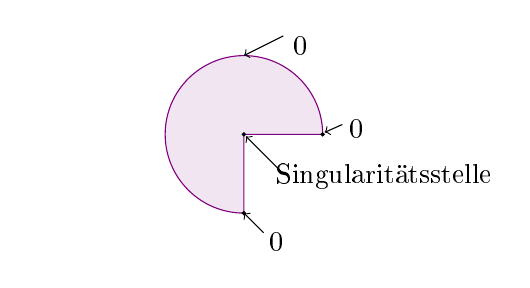
\begin{tikzpicture}[rotate=180, scale=0.25]
    \draw[violet, fill=violet!10] (4,0) arc(90:-180:4) -- (4,-4) 
      -- node[above, black]{} (4,-2)  -- (4,0);
    \draw[<-]  (3.9,-3.9) -- node[below]{ \qquad \qquad \qquad \qquad \ \  Singularitätsstelle} (2,-2);
     \draw[<-]  (-0.1,-4.1) -- node[]{    \ \ \ \ \ 0} (-1,-4.5);
          \draw[<-]  (4,0) -- node[below]{ \ \ \ \ \  0} (3,1);
                    \draw[<-]  (4,-8) -- node[]{ \ \ \ \ \  \ \ \ 0} (2,-9);

    \draw[fill=black] (4,-4) circle(.08);
        \draw[fill=black] (0,-4) circle(.08);
            \draw[fill=black] (4,0)  circle(.08);
  \end{tikzpicture}
\end{Beispiel}
	\underline{Holomorph in S $\Longrightarrow \Delta u_0 =0$}\\ \newline
Falls  $\nabla u_0 \notin L_2(S)$, \ $\Delta u=0$ und $ \nabla u \in L_2$ gilt \\ $\Longrightarrow$ \qquad u ist eindeutig durch die Randwerte bestimmt.

\underline{\textbf{Spezielle Lösungen der Poisson-Gleichung}}
\begin{align*}
        &\text{def. Fundementallösungen  }   &&  \phi(x) = \begin{cases}-\frac{1}{2\pi} \log|x|  &D=2\\-\frac{1}{4\pi} \frac{1}{|x|} &D=3 \end{cases} \\
        &\nabla \phi(x) = \begin{cases}-\frac{1}{2\pi} \frac{1}{|x|^2}x &D=2 \\ -\frac{1}{4\pi} \frac{1}{|x|^3}x & D=1\end{cases}  && \text{} \\
        &\text{radiale Koordinaten}	    &&\Delta \phi(x) = \begin{cases}\frac{1}{r}\partial_r \big(r \partial_r \varphi(r)\big) &2D \qquad \\\frac{1}{r^2}\partial_r^2 \big(r \varphi(r)\big) &3D \qquad  \end{cases}\Delta \phi =0 \text{ in } \ \R^D \backslash \{ 0\}
            \end{align*}

\begin{Definition}
    \begin{eqnarray*}
    \underline{\text{Def:}} &&u(x) = \int_{\Omega} \phi (x-y) f(y) \dy \\
    &&-\Delta x \int_{B_R (x)}\phi(x-y) \dy = -  \int_{B_R (x)} \Delta x\phi(x-y) \dy = -  \int_{|x-y|=R} \Delta x\phi(x-y) \frac{x-y_0}{|x-y_0|} \da\\
    &&\frac{1}{|\partial B_1 (x)|}\int_{|x-y_0|=R} \frac{x-y}{|x-y|^D} \frac{x-y_0}{x-y_0} \da  \ \mathop{\mathrm{\longrightarrow}}\limits_{R \rightarrow 0} \ 1
    \end{eqnarray*}
  $  \Longrightarrow \qquad - \Delta u(x)= f(x)$
  \end{Definition}

\textbf{Ein Beispiel für ein Finites Element} \\
Sei $\Omega \subset \R^2$ ein beschränktes Polygongebiet und $\overline\Omega = \cup \overline{K}$ eine Zerlegung in Dreiecke. \\
Finites Element $(K,V_K,\Lambda_K)$ mit K-Zelle. Hier ist $\overline{K}= \conv\{ z_0, z_1, z_2\}$

 \begin{align*}
        &V:K = \P_1(K)   && \qquad \qquad \text{Ansatzraum} \\
        &\Lambda_K=\span\{ \lambda_0, \lambda_1, \lambda_2\} \subset V_K`\subset \bC(K) && \hspace{-2.55cm}\text{Feiheitsgrade mit}\  <\lambda_k,\phi>=\phi(z_K) \\
        &\underline{\text{def. }} V_h = \{ v_h \in \bC(\overline{\Omega}) : v_K \in V_K\}
            \end{align*}
            \\
            
            
            
            \textbf{Aufgaben}
\begin{enumerate}[1)]
  \item Def. eindeutige Approximation $u_h \in V_h$ zu $u$.
      \item Wie gut lässt sich u in V-h approximieren?
      \item Wie gro\ss ist der Fehler? Bezüglich welchem Ma\ss ?
      \item Wir gro\ss ist der Lösungsaufwand?
      \end{enumerate}

            \textbf{Herausforderungen}
\begin{enumerate}[A)]
  \item Abstrakte Approximations und Lösungsidee- Theorie, die möglichst viele Anwendungen hat.
      \item Gro\ss e Vielfalt von Methoden, um für konkrete Anwendungen eine optional Methode zu finden.
     
          \end{enumerate}
          
          \textbf{Wiederholung:}
          \textbf{1. PDE Modelle}
          \textbf{1.1 Elliptische Modellprobleme} \\Laplace $\Delta u = 0$ ; Poisson $-\Delta u = f$ in $\Omega \subset \R^D \rightarrow$ Randwerte erforderlich! Bsp in 2 D GRAFIK1 
\subsection{Diffusions-Konvektions-Reaktionssysteme}

    \begin{align*}
        \text{gesucht:}&  &&u&&:&& \overline{\Omega} \times I \rightarrow \R && \Omega \subset \R^D \text{ beschränktes Gebiet } \ \ &&I=[0,T] \text{ Zeitintervall }\\
        \text{Daten:}& &&\kappa&& :&&  \overline{\Omega} \rightarrow \R^{D\times D}        && \text{Diffusionstensor} \\
                & &&q&&:&&  \overline{\Omega} \rightarrow \R^{D\times D}                        && \text{Flussvektor} \\
                & &&r&&:&&  \Omega \rightarrow \R                      && \text{Reaktionsrate} \\
                & &&f&&:&&  \Omega \rightarrow \R                        && \text{Quellen und Senken} \\
                & &&u_D&&:&&  \Gamma_D \times I \rightarrow \R                       && \text{Dirichlet Randwerte} \\
                & &&u_N&&:&&  \Gamma_N \times I  \rightarrow \R                        && \text{Neumann-Randbedingung} &&\text{,wobei }\Gamma_N \cup \Gamma_R \cup \Gamma_D = \partial \Omega \\
                & &&u_R&&:&& \Gamma_R \times I  \rightarrow \R                        && \text{Robin-Randbedingung} \\ 
                & &&\alpha&&:&&  \Gamma_R \times I  \rightarrow \R                       && \text{Randkapazität}           \end{align*}

\textbf{Konstitutionsgleichung}\\
    \begin{align*}
        \text{Fluss:}\qquad \sigma =-\kappa \nabla u \\
    \end{align*}
\textbf{Bilanzgleichung}
 \begin{align*}
        &\omega \subset \Omega \text{ (hinreichend regulär)}    \qquad &&\partial_t \int_\omega u \dx =  \underbrace{ -\int_{\partial \omega} \sigma \cdot n_\omega \da}
	    _{\int_\omega \div \sigma \dx} +\int_\omega f \dx + \int_\omega ru \dx  \\
    \end{align*}
        \textbf{Diffusions-Konvektions-Reaktionssystem:}
        \begin{align*} % requires amsmath; align* for no eq. number
\partial_t u= -\div \sigma + f +ru \qquad \Longrightarrow \qquad &\partial_t u -\div \kappa \nabla u + \div(qu)-ru = f \\ &\partial_t u -\div \kappa \nabla u + q\nabla u + \underbrace{(\div q- r)u}_{\rs} = f        \end{align*}
      
        
        Randwerte:
            \begin{align*}
        &u = u_D    &&\text{auf } \Gamma_D \times I \\
        &\sigma \cdot n = g_N    &&\text{auf } \Gamma_N \times I \\
        &\sigma \cdot n  + \alpha u = g_R    &&\text{auf } \Gamma_R \times I \\
    \end{align*}
    \textbf{Spezialfälle:}
    \begin{enumerate}[A)]
  \item stationär $$-\div x \nabla + 1 \cdot \nabla u + \hat{r}u= f \qquad \text{  (unabhängig von t)}$$
      \item            \begin{align*}
        &x = I_D 1=0, r=0    &&-\Delta u =f && \text{Poisson-Gleichung elliptisches Modellproblem} \\
        &    &&\underbrace{\partial_t u =\Delta u}_{\text{spezielle Lösung in } \R^D: \qquad u(x,t)= (4 \pi t)^{-D/2} \int_{\R^D} \exp(- \frac{|x-y|}{4t}u_0(y) \dy \text{ mit } u(x,0)= u_0(x)} &&\text{Wärmeleitungsproblem parabolische Modellproblem}\\
    \end{align*} 
     $\Omega =(0,L)^2$ Einheitsquadrat  der Kantenlänge L \\
     $w_{n,k}(x,y) = \sin(x:n \frac{\pi}{L} \sin(y_k \frac{\pi}{L}) \Rightarrow w_{n,k}(x,y)=\underbrace{- \Big( (n\frac{\pi}{L})^2-(k\frac{\pi}{L})^2 \Big)}_{\lambda_{n,k}} w_{n,k}(x,y)$\\ $ \Rightarrow - \Delta u =f \text{ mit} f= \sum_{n,k \in \N} \alpha_{n,k} w_{n,k} \text{ mit } \alpha_{n,k} \frac{(w_{n,k},f)_0}{||w_{n,k}||_0}$\\
     $u_{n,k}(x,y,t)= \exp(-\lambda_{n,k} t) w_{n,k} (x,y \Rightarrow \partial_t u_{n,k}= - \lambda_{n,k} u_{n,k}= \Delta u_{n,k}$\\
    
   $ u = \sum \beta_{n,k} u_{n,k}, \qquad \beta_{n,k}= \frac{u_0,w_{n,k}}{||w_{n,k}||_0} \Rightarrow \partial_t u =\Delta u$ mit $u=0 auf \partial \Omega$ und $u(0)=u_0$ in $\Omega$
   \item Allgemeine Diffusion: Richtung $d_1, d_2$ der stärksten und schwächsten Diffusion \\ GRAFIK2 \\  
         \begin{align*}
        &|d_1|=|d_2|=1    &&, d_1 senkrechtZEICHEN d_2 \\
        &\text{in 3D}    &&d_3 = d_2 \times d_2 \\
    \end{align*}
    Diffusionskoeffizienten $x_k >0$\\ $\sigma =- \sum x_k ( \nabla u \cdot d_k) d_k = -x \nabla u $ mit $x= \sum \kappa_k d_k d_k^T$ symetrisch positif definit\\ betrachte $\varphi: \hat{\Omega} \rightarrow \Omega$ linear affine Transformation: $\varphi(\hat{x})= x_0 + F \hat{x}$ mit $F\in \R^{D\times D}, \det F >0, F= D_{\varphi}$
   \\ def. $ \hat{u}(\hat{x})=u(x)$ mit $x = \varphi (\hat{x})$ \\
   
 $  D_{\hat{x}} u(\varphi(\hat{x})= D_x u(x) D_{\hat{x}}\varphi(\hat{x})=D_x u(x) F \Rightarrow \underbrace{\nabla_{\hat{x}} u(\varphi(\hat{x}))}_{\nabla_{\hat{x}} \hat{u}(\hat{x})}= \Big( D_{\hat{x}} u(\varphi(\hat{x}))\Big)= F^T \nabla_x u(x)$\\
 def. $\hat{\sigma}(\hat{x})= \sigma(x)= \sigma(\varphi(\hat{x}))$ \\ $\Rightarrow D_{\hat{x}} \sigma (\varphi(\hat{x}))= D_x \sigma(x) F$\\ $\Rightarrow \div_x \sigma(x)= \tr D_x \sigma(x)= \tr (D_{\hat{x}}\hat{\sigma} (\hat{x}) F^{-1}) = \tr (F^{-1} D_{\hat{x}} \hat{\sigma}(\hat{x}))= \tr (d_{\hat{x}}F^{-1} \hat{\sigma}(\hat{x}) = \div(F^{-1})\hat{\sigma}(\hat{x})) $ \\
 $\hat{\kappa}(\hat{x})= \kappa (x) \Rightarrow \div_ {\hat{x}} F^{-1}(\hat{\kappa}F^{-1} \nabla_{\hat{x}} \hat{u}(\hat{x}) ) = \div_x \kappa \nabla_x u(x)$\\
 wähle $FF^T= \kappa \Rightarrow \Delta_{\hat{x}} \hat{u}(\hat{x}) = \div_x \kappa \nabla_x u (x) $
 \item Reaktion ***
 \item Transport $\partial_t u + \div(qu)=f$
\\ spezielle Lösung: $q \in \R^D \qquad u(x,t) = a(|q|^2t-q\cdot x) |q|^2 \qquad a \in C^1(\R)$\\
$\Rightarrow \partial_t u = a'(|q|^2t-q\cdot x) q \qquad \div(qu) = q \cdot \nabla u = |q|^2 a' $\\ $\div q=0$ Charakteristik $\gamma: [0,T] \rightarrow \Omega$ mit $\hat{\gamma}(t)=q(\gamma(t))$ \\ $\rightarrow \partial_t u(\gamma(t),t)=const$
   
   
          \end{enumerate}




          
          
\newpage

\section{Einführung}

\textbf{Ziel:} Analyse von Diskretisierungs- und Lösungsmethoden für PDEs partial differential equations.

\subsection{PDE-Modelle}

\subsection{Diffusion (als Prototyp = Modellproblem)}
$\Omega \in \R^D$
Partielle Differentialgleichungen (PDE) sind Gleichungen, die partielle
Ableitungen einer unbekannten Funktion $u$ in mehreren Variablen enthalten.
Im Folgenden nehmen wir an, dass alle Grö\ss en hinreichend glatt sind.


\begin{Bezeichnung}
    \begin{align*}
        &u = u(x,t)     && \text{Zustandsgrö\ss e} \\
        &x = \left(\begin{smallmatrix}
                x_1 \\
                \vdots \\
                x_d
              \end{smallmatrix}\right)\in\Omega\subset\R^d
                        && \text{Ortsvariable} \\
        &t\in [0,T]	    && \text{Zeitvariable} \\
        &\partial_t = \frac{\partial}{\partial t}
                        && \text{partielle Ableitung nach der Zeit}
    \end{align*}
\end{Bezeichnung}


Sei $S(u)$ eine (Volumen-)Dichte oder Konzentration.
Für jedes Kontroll-Volumen $V\subset\Omega$ beschreibt
\begin{eqnarray*}
     \partial_t \int_{V} S(u(x, t))\,dx
\end{eqnarray*}
die zeitliche änderung von $S(u)$ in $V$.


Die änderung entsteht durch:


\begin{enumerate}[1)]
  \item
      Quellen und Senken $Q = Q(x, t, u(x,t))$: \\
      Falls $Q > 0$, dann wird $S(u)$ erzeugt. \\
      Falls $Q < 0$, dann wird $S(u)$ verringert.
  \item
      Fluss $J(x,t)$ durch den Rand von $\partial V$: \\
      $J = \left(\begin{smallmatrix}
              J_1 \\ \vdots \\ J_d
	      \end{smallmatrix}\right)$,
      $J_i$ Fluss-Dichte in $x_i$-Richtung. \\
      $J\nu = \sum_{i=0}^d \nu_i J_i$ Fluss über den Rand. \\
      (dabei ist $\nu\colon \partial V \to \R^d$ mit $|\nu| = 1$ die
      äu\ss{}ere Einheitsnormale)
\end{enumerate}


Die (Massen-) Erhaltung ergibt, falls das Volumen $V$ nicht von der Zeit
abhängt
\begin{eqnarray*}
      \int_V \partial_t S(u(x,t)) \dx
    = - \int_{\partial V} J(x,t) \nu \da + \int_V Q(x,t,u(x,t))) \dx.
\end{eqnarray*}
Sie sagt aus das weder Masse erzeugt noch erschaffen werden kann. Die
zeitlichen änderungen im Volumen $V$ sind Folgen des (Masse-) Transports
über den Rand $\partial V$.


\textbf{Satz von Gau\ss}

  Sei $V\subset\R^d$ beschränkt mit stückweise glattem Rand. Sei $F\in
  C^1(V,\R^d)$ ein Vektorfeld. Dann gilt
  \begin{eqnarray*}
      \int_V \operatorname{div} F(x) \dx = \int_{\partial V} F(x) \nu(x) \da,
  \end{eqnarray*}
  mit der Divergenz $\operatorname{div} F = \nabla \cdot F = \sum_{i=0}^d
  \partial_i F_i, \
  \nabla = \left(\begin{smallmatrix}
                \partial_1 \\ \vdots \\ \partial_d
           \end{smallmatrix}\right) \text{ und}
  \ \partial_i = \frac{\partial}{\partial x_i}$.


\begin{Anwendung}
    Es gilt also für alle $V\subset \Omega$
    \begin{eqnarray*}
        \int_V \partial_tS(u(x,t)) + \operatorname{div} J(x,t)
        - Q(x,t,u(x,t)))\,dx = 0.
    \end{eqnarray*}
    Da $V\subset\Omega$ beliebig folgt daraus die
    \emph{Erhaltungsgleichung} in differentieller Form
    \begin{eqnarray*}
        \partial_tS(u(x,t)) + \operatorname{div} J(x,t) - Q(x,t,u(x,t)) = 0,
        \qquad \forall x\in \Omega, \ t\in [0,T].
    \end{eqnarray*}
\end{Anwendung}


Die Erhaltungsgleichung muss durch (phenomenologische)
\emph{konstitutive Gesetze} geschlossen werden, die eine Beziehung zwischen den
Zustandsgrö\ss en $u$ und den Fluss $J$ postulieren.


\begin{Beispiel}
    $\Omega$ sei mit einer Flüssigkeit gefüllt und $S(u) = u$ die
    Konzentration einer gelösten Substanz. \\
    \emph{Szenario I} \\
    Flüssigkeit ruht, die Konzentration strebt ins Gleichgewicht von hoher zu
    niedriger Konzentration:
    \begin{eqnarray*}
        J^{(1)} = -K\nabla u, \qquad K > 0 \qquad \left[\frac{m^2}{s}\right]
        \qquad \text{(Materialparameter)}\\
    \end{eqnarray*}
    und wir erhalten die \emph{Diffusionsgleichung}
    \begin{eqnarray*}
        \partial_t u - \nabla \cdot (K \nabla u) = Q.
    \end{eqnarray*}
    \emph{Szenario II} \\
    Flüssigkeit bewegt sich mit der Geschwindigkeit $c\colon \Omega \to \R^d$:
    \begin{eqnarray*}
        J^{(2)} = cu
    \end{eqnarray*}
    sodass die \emph{Transportgleichung} gegeben ist durch
    \begin{eqnarray*}
        \partial_t u + \nabla \cdot (cu) = 0.
    \end{eqnarray*}
    Zusammen ergibt sich die \emph{Konvektions-Diffusions-Gleichung}
    \begin{eqnarray*}
        \partial_t u - \nabla \cdot (K \nabla u  - cu) = Q.
    \end{eqnarray*}
\end{Beispiel}


\begin{Entdimensionalisierung}
    Fixiere Refernzgrö\ss en $x_\text{ref}, \ u_\text{ref}$ und $t_\text{ref}$.
    Reskaliere dazu
    \begin{eqnarray*}
        x\mapsto \frac{x_i}{x_\text{ref}}, &
        u\mapsto \frac{u_i}{u_\text{ref}}, &
        t\mapsto \frac{t_i}{t_\text{ref}}.
    \end{eqnarray*}
    Somit erhält man keine Einheiten. Die typische Grö\ss enordnung ist 1.
\end{Entdimensionalisierung}



\subsection{Randbedingungen}


Betrachte $\partial_t S(x,u(x,t)) + \nabla \cdot (C(x,u(x,t)) - K(x,\nabla
u(x,t))) = Q(x,t,u(x,t))$ im Raum-Zeit-Zylinder $(x,t)\in \Omega\times (0,T)
\subset \R^d\times \R$.

Im Wesentlichen unterscheiden wir drei Randbedingungen, wozu wir den Rand in
drei disjunkte Teile unterteilen:
$\partial\Omega = \Gamma_1\cup \Gamma_2\cup \Gamma_3\colon$

\begin{enumerate}[1)]
    \item
	Fluss Randbedingungen auf $\Gamma_1$ (Neumann RB)
	\begin{eqnarray*}
	    -(C(u) - K(\nabla u)) \cdot \nu = g_1
	\end{eqnarray*}
    \item
	Gemischte Randbedingungen auf $\Gamma_2$ (Robin RB)
	\begin{eqnarray*}
	    -(C(u) - K(\nabla u)) \cdot \nu + \alpha u = g_2
	\end{eqnarray*}
     \item
	Dirichlet Randbedingungen auf $\Gamma_3$ (wesentliche RB)
	\begin{eqnarray*}
	    u = g_3
	\end{eqnarray*}
\end{enumerate}


Es liegen homogene Randbedingungen vor falls $g_i = 0$.


\begin{Spezialfälle}
    Wir erhalten:
    \begin{enumerate}[1)]
	\item
	    den Sturm Liouville Operator für $d=1$ im Raum.
	\item
	    eine stationäre Gleichung, falls keine Zeitableitung vorliegt.
	\item
	    die lineare Gleichung $Q(x,u) = f(x) - \underbrace{q(x)u(x)}
	    _{\text{Reaktionsterm}}$
	    mit $C(u) = cu, \ K(\nabla u) = K\nabla u$.
	\item
	    die Poisson-Gleichung $-\Delta u = f$ für $c\equiv 0, \
	    K\equiv 1, \ q\equiv 0$.
	\item
	    die Laplace-Gleichung $-\Delta u = 0$ für $f\equiv 0$.
    \end{enumerate}
\end{Spezialfälle}



\subsection{Modell-Problem (die Poisson-Gleichung)}


\begin{Definition}
\label{def:1.1}
    Sei $\Omega\subset \R$ beschränkt mit stückweise glattem Rand. Sei
    $f\in C(\Omega), \ g\in C(\partial\Omega)$. Dann hei\ss t $u\in C^2(\Omega)
    \cap C(\overline\Omega)$ mit
    \begin{eqnarray*}
          -\Delta u(x)
        &=& f(x), \quad x\in \Omega \qquad \ \ (\text{in } \Omega) \\
            u(x)
        &=& g(x), \quad x\in \partial\Omega \qquad (\text{auf } \partial\Omega)
    \end{eqnarray*}
    eine (klassische) Lösung der Poisson-Gleichung (mit Dirichlet
    Randbedingungen).
\end{Definition}


\begin{Beispiel}
    Mit Hilfe von Fundamentallösungen kann eine Lösung der Poisson-
    Gleichung konstruiert werden. Hierbei ist $K(x,y) = \Psi(|x-y|)$ die
    Fundamentallösung, wobei
    \begin{eqnarray*}
        \Psi(r) = \begin{cases}
                      \frac{r^{2-d}}{(2-d)\omega_d}, 	& d>2 \\
                      \frac{\log{r}}{2\pi}, 		& d=2
                  \end{cases},
    \end{eqnarray*}
    und $\omega_d$ das Volumen der Einheitssphäre ist. Sie erfüllt
    $\Delta_x K(x,y) = 0$ für $x\neq y$. Falls $u\in C^2(\overline\Omega)$
    ist, dann ist eine Lösung der Poisson-Gleichung gegeben durch
    \begin{eqnarray*}
          u(y)
        = \int_{\partial \Omega} \big(\partial_\nu K(x,y) g(x) - K(x,y) h(x) \big) \da_x
          -\int_\Omega K(x,y) f(x) \dx
    \end{eqnarray*}
    mit der äu\ss{}eren Einheitsnormalen $\nu\colon \partial\Omega \to
    \R^d, \ |\nu| = 1, \ h(x) = \partial_\nu u(x)$, wobei die Normalenableitung
    $\partial_\nu = \nu\cdot\nabla = \sum_{i=0}^d \nu_i \partial_i$ und
    $g(x) = u(x), \ f(x) = -\Delta u(x)$.

    $\textbf{Problem:}$ Wenn $f$ und $g$ vorgegeben sind, muss $h$ bestimmt
    werden!
\end{Beispiel}


\begin{Bezeichnung}
    Eine Funktion $u \in C^2(\Omega)$ heißt harmonisch, falls $\Delta u = 0$ in $\Omega$ gilt.
\end{Bezeichnung}


\begin{Bemerkung}
    Wenn $\Delta u \le 0$, dann ist $u(y) \le \frac{1}{R^d \omega_d}
    \int_{|x-y|=R} u(x) \da$.
\end{Bemerkung}


\begin{Maximumsprinzip}
\label{max:1.2}
    Sei $u\in C^2(\Omega)\cap C(\overline\Omega)$ mit $\Delta u \le 0$.
    Dann gilt
    \begin{eqnarray*}
        \sup_{x\in \Omega} u(x) = \sup_{x\in \partial\Omega} u(x).
    \end{eqnarray*}
\end{Maximumsprinzip}


\begin{proof}
    Ohne Beweis!
\end{proof}


\begin{Folgerung}
    \label{fol:1.3}
    Das Poisson-Problem \eqref{def:1.1} hat höchstens eine Lösung.
\end{Folgerung}


\begin{proof}
    Seien $u$ und $v$ Lösungen von
    \begin{eqnarray*}
        -\Delta u(x) &=& f(x), \
        -\Delta  v(x) = f(x)
        \qquad \text{ in } \Omega \\
        u(x) &=& g(x),
        \ \ \quad \ v(x) = g(x)
        \qquad \text{ auf } \partial\Omega. 
    \end{eqnarray*}
    Dann  löst $w(x) = u(x) - v(x)$
    \begin{eqnarray*}
        -\Delta w(x) &=& 0 \qquad \text{ in } \Omega \\
        w(x) &=& 0 \qquad \text{ auf } \partial\Omega.
    \end{eqnarray*}
    Mit \eqref{max:1.2} folgt
    \begin{eqnarray*}
        \sup_{x\in \Omega} w(x) = \sup_{x\in \partial\Omega} w(x) = 0
        \quad \text{und } \inf_{x\in \Omega} w(x) = 0.
    \end{eqnarray*}
    Also $w(x) \equiv 0$.
\end{proof}


\begin{Definition}
    \label{def:1.4}
    $\Omega\subset \R^d$ ist ein Lipschitz-Gebiet, wenn
    \begin{enumerate}[a)]
	\item
	    $\Omega$ ist offen in $\R^d$,
	\item
	    $\Omega$ ist zusammenhängend,
	\item
	    $\partial\Omega$ ist eine Lipschitz-Mannigfaltigkeit, d.h. für alle
	    $y\in \partial\Omega$ existiert eine lokale Karte $\Psi\in C^{0,1}
        (V, \R^d)$ mit $V\subset \R^{d-1}$ offen und $y\in \Psi(V)
        \subset \partial\Omega$.
    \end{enumerate}
\end{Definition}


\begin{Beispiel}
    Das Einheitsquadrat
    $\Omega = (0,1)^2$ ist ein Lipschitz-Gebiet. Offensichtlich ist $\Omega$
    offen und zusammenhängend. Für die Lipschitz-Mannigfaltigkeit $\partial \Omega$ ist
    beispielsweise für
    $\ y =  \left(\begin{smallmatrix}
		0 \\ 0
	    \end{smallmatrix}\right)$
    die Abbildung
    $\Psi(t) = \left(\begin{smallmatrix}
		  t + |t| \\ -t + |t|
              \end{smallmatrix}\right)$
    für $t \in V = (-\frac{1}{2},\frac{1}{2})$ eine lokale Karte mit $y = \Psi(0)$.
\end{Beispiel}


\begin{Satz}
    \label{satz:1.5}
    In einem Lipschitz-Gebiet hat das Poisson-Problem \eqref{def:1.1} mit
    Dirichlet Randbedingungen eine eindeutige Lösung.
\end{Satz}


\begin{proof}
    Ohne Beweis!
\end{proof}

%\section{Finite Differenzen}


\begin{Definition}
    \label{def:2.1}
    Sei $u\in C(\Omega)$, $x\in \Omega\subset \R^d$ offen und $h > 0$
    hinreichend klein. Dann definiere
    \begin{enumerate}[a)]
	\item
	    den einseitigen und zentralen Differenzenquotienten durch
	    \begin{eqnarray*}
                \partial_i^+ u(x)
            &=& \frac{1}{h} \left(u\left(x + h e^i\right) - u(x)\right), \\
                \partial_i^- u(x)
            &=& \frac{1}{h} \left(u(x) - u\left(x - h e^i\right)\right), \\
                \partial_i^0 u(x)
            &=& \frac{1}{2h} \left(u\left(x + h e^i\right)
                - u\left(x - h e^i\right)\right).
	    \end{eqnarray*}
	\item
	    den Differnzenquotienten 2. Ordnung durch
	    \begin{eqnarray*}
                \partial_i^+ \partial_i^- u(x)
            &=& \frac{1}{h^2} \left(u\left(x + h e^i\right) - 2u(x)
                + u\left(x - h e^i\right)\right).
	    \end{eqnarray*}
	\item
	    den diskreten Laplace-Operator durch
	    \begin{eqnarray*}
                \Delta_h u(x)
            &=& \sum_{i=1}^d \partial_i^+ \partial_i^- u(x).
	    \end{eqnarray*}
    \end{enumerate}
\end{Definition}


\begin{Beispiel}
    Für $u\in C(\Omega)$ und den diskreten Laplace-Operator gilt dann
    \begin{eqnarray*}
            \Delta_h u(x_1, x_2)
        &=& \frac{1}{h^2} (u(x_1 + h, x_2) + u(x_1 - h, x_2) - 4u(x) \\
            && + u(x_1, x_2 + h) + u(x_1, x_2 - h)).
    \end{eqnarray*}
\end{Beispiel}


\begin{Bemerkung}
    Wenn $u$ hinreichend glatt ist, gilt
    \begin{enumerate}[a)]
	\item
	    für den einseitigen und zentralen Differenzenquotienten
	    \begin{eqnarray*}
                |\partial_i^+ u(x) - \partial_i u(x)|
            &\le& Ch \|\partial_{h, i}^2 u\|_\infty, \\
                |\partial_i^- u(x) - \partial_i u(x)|
            &\le& Ch \|\partial_i^2 u\|_\infty, \\
                |\partial_i^0 u(x) - \partial_i u(x)|
            &\le& Ch^2 \|\partial_i^3 u\|_\infty. \\
	    \end{eqnarray*}
	\item
	    für den Differenzenquotienten 2. Ordnung
	    \begin{eqnarray*}
                |\partial_i^+\partial_i^- u(x) -
                \partial_i^2 u(x)|
            &\le& Ch^2 \|\partial_i^4 u\|_\infty.
	    \end{eqnarray*}
	\item
	    für den diskreten Laplace-Operator
	    \begin{eqnarray*}
                |\Delta_h u(x) - \Delta u(x)|
            &\le& Ch^2 \sum_{i=1}^d \|\partial_i^4 u\|_\infty.
	    \end{eqnarray*}
    \end{enumerate}
\end{Bemerkung}


\begin{Kartesische Gitter in 2-d}
    Sei $\Omega = [a_1, b_1] \times [a_2, b_2]$ und $\ N_1, \ N_2\in \N$. \\
    Wir definieren dann die Schrittweiten und Gitterpunkte durch
    \begin{eqnarray*}
        h_k = \frac{b_k - a_k}{N_k + 1}, \quad
        x_{n j} =	\begin{pmatrix}
                        a_1 + n h_1 \\
                        a_2 + j h_2
                    \end{pmatrix}.
    \end{eqnarray*}
    Der Raum der inneren Gitterpunkte und der Randpunkte ist definiert
    durch
    \begin{eqnarray*}
            \Omega_h
        &=& \{x_{n, j} \colon 1 \le n \le N_1, \ 1 \le j \le N_2\}, \\
            \partial\Omega_h
        &=& \{x_{n, j} \colon 0 \le n \le N_1 + 1 \text{ und } j = 0
            \text{ oder } j = N_2 + 1, \\
            && 0 \le j \le N_2 + 1 \text{ und } n = 0 \text{ oder }
            n = N_1 + 1\}.
    \end{eqnarray*}
    Die Gesamtheit aller Gitterpunkte ist dann
    $\overline\Omega_h = \Omega_h \cup \partial\Omega_h$.
\end{Kartesische Gitter in 2-d}

Desweiteren sei $V_h = \{u_h \colon \overline\Omega_h \rightarrow \R\}$ der
Raum der Gitterfunktionen, und
\begin{eqnarray*}
    I_h \colon C(\overline\Omega) &\rightarrow& V_h, \\
    u &\mapsto& (I_h u)(x) = u(x) \quad \text{für alle } x\in
    \overline\Omega_h
\end{eqnarray*}
die Gitterinterpolation. Dann setzen wir
\begin{eqnarray*}
      \|u_h\|_{\infty, \overline\Omega_h}
    = \|u_h\|_\infty
    = \max_{x\in \overline\Omega_h} |u_h(x)|.
\end{eqnarray*}


\subsection{Finite-Differenzen-Diskretisierung (FD)}


\begin{enumerate}[A)]
    \item 	
	Poisson-Problem (mit Dirichlet-Ranbedingungen) und $u\in
	C^2(\Omega) \cap C(\overline\Omega)$. Die PDE ist
	\begin{eqnarray*}
            -\Delta u(x)
	    &=& f(x) \qquad x\in \Omega \\
            u(x)
	    &=& g(x) \qquad x\in \partial\Omega.
	\end{eqnarray*}
	Die FD-Diskretisierung mit $u_h\in V_h$ ist dann gegeben durch
	\begin{eqnarray*}
            -\Delta_h u_h(x)
	    &=& f(x) \qquad x\in \Omega_h \\
            u_h(x)
	    &=& g(x) \qquad x\in \partial\Omega_h.
	\end{eqnarray*}
     \item
	Konvektions-Diffusions-Problem mit $u\in C^2(\Omega) \cap
    C(\overline\Omega)$.
	Für die PDE gilt
	\begin{eqnarray*}
            L u(x)
	    &=& f(x) \qquad x\in \Omega \\
            u(x)
	    &=& g(x) \qquad x\in \partial\Omega.
	\end{eqnarray*}
    mit $Lu = -\nabla \cdot (K\nabla u) + \nabla \cdot (cu) + qu$.

	Die FD-Diskretisierung mit $u_h\in V_h$ ist dann gegeben durch
	\begin{eqnarray*}
            L_h u_h
	    &=& f_h = I_h f \qquad x\in \Omega_h \\
            u_h
	    &=& g_h = I_h g \qquad x\in \partial\Omega_h \\
	\end{eqnarray*}
    mit
    \begin{eqnarray*}
            L_h u_h(x)
        &=& \sum_{i=1}^d \frac{1}{h^2} \biggl(K\left(x + \frac{h}{2} e^i\right)
            \left( u(x + h e^i) - u(x) \right) \\ 
            && + K\left(x - \frac{h}{2} e^i\right)\bigl(u(x)
               - u(x - h e^i) \bigr) \biggr) \\
            && + \sum_{i=1}^d  \frac{1}{h}  \big(c_i(x)
                 \left(u(x + h e^i)
               - u(x - h e^i)\right)\big) \\
            && + (\nabla c(x) + q(x)) u(x).
    \end{eqnarray*}
\end{enumerate}


\begin{Beispiel}[$d = 2$]
    Der Differenzenoperator lässt sich durch sogenannte
    \emph{Differenzensterne} darstellen, wobei hier $h_1 = h_2$ gewählt wurde.
    \begin{enumerate}[A)]
	\item
	    \emph{Laplace-Operator}: \\
	    Dieser lässt sich durch einen Fünfpunkte-
	    Differenzenstern dastellen:
	    \begin{eqnarray*}
              -\Delta_h
            = \frac{1}{h^2}
              \begin{bmatrix}
                  & & -1 & & \\
                  -1 & & 4 & & -1 \\
                  & & -1 & &
              \end{bmatrix},
	    \end{eqnarray*}
	    d.h
	    \begin{eqnarray*}
              -\Delta_h u_h(x)
            = \frac{1}{h^2} \left(4 u(x) - u\left(x + h e^1\right)
              - u\left(x - h e^1\right) - u\left(x + h e^2\right)
              - u\left(x - h e^2\right)\right).
	    \end{eqnarray*}
	\item
	    \emph{Konvektions-Diffusions-Operator}: \\
	    Der Operator
        $L u = -\nabla \cdot (K \nabla u) + \nabla \cdot (c u) + q u$
        kann auch durch einen Fünfpunkte-Diskretisierungsoperator
        dargestellt werden:
	    \begin{eqnarray*}
                L_h
            &=& \frac{1}{h^2} \left[
                \begin{smallmatrix}
                    & & -K\left(x - \frac{h}{2} e^2\right) & & \\
                    -K\left(x - \frac{h}{2} e^1\right) & &
                    K\left(x + \frac{h}{2} e^1\right)
                    + K\left(x + \frac{h}{2} e^1\right)
                    + K\left(x - \frac{h}{2} e^2\right)
                    + K\left(x - \frac{h}{2} e^2\right) & &
                    -K\left(x + \frac{h}{2} e^1\right) \\
                    & & -K\left(x - \frac{h}{2} e^2\right) & &
                \end{smallmatrix} \right] \\
		    &&+ \frac{1}{h} \left[
                \begin{smallmatrix}
                    & & c_2(x) & & \\
                    -c_1(x) & & 0 & & c_1(x) \\
                    & & -c_2(x) & &
                \end{smallmatrix} \right]
		    + \left[\begin{smallmatrix}
                  &  0 &  \\
                  0 & \nabla c(x) + q(x) & 0 \\
                  &  0 & \\
              \end{smallmatrix}\right],
	    \end{eqnarray*}
	    d.h.
	    \begin{eqnarray*}
            L_h u_h(x)
        &=& \sum_{i=1}^d \frac{1}{h^2} \biggl(K\left(x + \frac{h}{2} e^i\right)
            \left( u(x + h e^i) - u(x) \right) \\ 
            && + K\left(x - \frac{h}{2} e^i\right)\bigl(u(x)
               - u(x - h e^i) \bigr) \biggr) \\
            && + \sum_{i=1}^d  \frac{1}{h}  \big(c_i(x)
                 \left(u(x + h e^i)
               - u(x - h e^i)\right)\big) \\
            && + (\nabla c(x) + q(x)) u(x).
	    \end{eqnarray*}
    \end{enumerate}
\end{Beispiel}



\begin{Satz}
    \label{satz:2.2}
    Sei $K\in C^2(\overline\Omega), \ c\in C^1(\overline\Omega, \R^d), \
    q\in C(\overline\Omega)$ und $\Omega\subset \R^d$ offen. Sei dazu
    $\Omega_h = a + h \Z^d$ ein Gitter mit $x\pm he^i\in \overline\Omega$ für
    alle $x\in \Omega_h$. Dann gilt für alle $u\in C^4(\overline\Omega)$
    \begin{eqnarray*}
            \|L_h u - Lu\|_{\infty,\Omega_h}
        \le C h^2 \sum_{i=1}^d \left(\|\partial_i^4 u\|_{\infty, \Omega}
            + \|\partial_i^3 u\|_{\infty, \Omega}\right)
    \end{eqnarray*}
    (mit C unabhängig von h), d.h. $L_h$ ist konsistent von der Ordnung $p=2$.
\end{Satz}


\begin{proof}
    Es gilt
    \begin{eqnarray*}
            S^+_i
        &=& K\left(x + \frac{h}{2} e^i\right) \left(u\left(x + h e^i\right)
            - u(x)\right) \\
        &=& K\left(x + \frac{h}{2} e^i\right) \left(h\partial_i
            u\left(x + \frac{h}{2} e^i\right)
            + \frac{h^3}{6 \cdot 8}\partial_i^3
            u\left(x + \frac{h}{2} e^i\right) + O(h^5)\right),
        \\
            S^-_i
        &=& K\left(x - \frac{h}{2} e^i\right) \left(u(x)
            - u\left(x - h e^i\right)\right) \\
        &=& K\left(x - \frac{h}{2} e^i\right) \left(h\partial_i
            u\left(x - \frac{h}{2} e^i\right)
            + \frac{h^3}{6 \cdot 8}\partial_i^3
            u\left(x - \frac{h}{2} e^i\right) + O(h^5)\right).
    \end{eqnarray*}
    Mittels Taylorentwicklung von
    \begin{eqnarray*}
            u\left(x \pm \frac{h}{2}e^i\right)
        &=& u(x) \pm \frac{h}{2}\partial_i u(x)
            + \frac{h^2}{8}\partial_i^2 u(x) + O(h^3)
    \end{eqnarray*}
    ergibt sich
    \begin{eqnarray*}
        u\left(x + \frac{h}{2} e^i\right) - u\left(x - \frac{h}{2} e^i\right)
        = h \partial_i u(x) + O(h^3).
    \end{eqnarray*}
    Zusammen mit der Taylorentwicklung von
    \begin{eqnarray*}
            K\left(x \pm \frac{h}{2}e^i\right)
        &=& K(x) \pm \frac{h}{2}\partial_i K(x)
            + \frac{h^2}{8}\partial_i^2 K(x) + O(h^3)
    \end{eqnarray*}
    folgt dann
    \begin{eqnarray*}
            S^+_i - S^-_i
        &=& K(x) \left(h\partial_i \left(u\left(x + \frac{h}{2} e^i\right)
            - u\left(x - \frac{h}{2} e^i\right)\right)\right) \\
        &&  + \frac{h^3}{6 \cdot 8}\partial_i^3
            \left(u\left(x + \frac{h}{2} e^i\right)
            - u\left(x - \frac{h}{2} e^i\right)\right) \\
        &&    + \frac{h}{2}\partial_i K(x)
            \left(h\partial_i \left(u\left(x + \frac{h}{2} e^i\right)
            - u\left(x - \frac{h}{2} e^i\right)\right)\right)
            + O(h^4) \\
        &=& h^2 K(x) \partial_i^2 u(x) + \frac{h^3}{2} \partial_i K(x)
            \partial_i^2 u(x) + O(h^4).
    \end{eqnarray*}
    Analog zur obigen Taylorentwicklung gilt
    \begin{eqnarray*}
        u\left(x + h e^i\right) - u\left(x - h e^i\right)
        = 2 h \partial_i u(x) + O(h^3).
    \end{eqnarray*}
    Dies liefert uns schlie\ss{}lich
    \begin{eqnarray*}
            |L_h u(x) - Lu(x)|
        &=& \Biggl|\sum_{i=1}^d \Biggl[\frac{1}{h^2} \left(K(x) h^2
            \partial_i^2 u(x)
            - \partial_i K(x) \frac{h^3}{2} \partial_i u(x)\right) \\
            &&+ \frac{1}{h} (c_i(x) 2 h \partial_i u(x))\Biggr]
            + K(x) \Delta u(x) \\
            &&+ \nabla K(x) \nabla u(x) - c(x) \nabla u(x) + O(h^2)\Biggr|
         =  O(h^2)
    \end{eqnarray*}
    Konsistenz der Ordnung $p = 2$.
\end{proof}


\begin{Implementation}
    Sei $\Omega_h = \left\{x^1, \dots, x^N\right\}$ mit $N = N_1 N_2$ eine
    Nummerierung der Gitterpunkte und
    \begin{eqnarray*}
          V_h(0)
        = \{u_h\in V_h \colon u_h(x) = 0 \text{ für } x\in \partial\Omega_h\}.
    \end{eqnarray*}
    Weiter sei
    \begin{eqnarray*}
        E_h \colon \R^N &\to& V_h(0) \\
        \underline u &\mapsto& u_h \qquad \text{mit } u_h(x^n)
        = \underline u_n.
    \end{eqnarray*}
    Dann definiere $u_h^g\in V_h$ mit
    \begin{eqnarray*}
        u_h^g(x) &=& g(x) \quad x\in \partial\Omega_h \\
        u_h^g(x) &=& 0 \quad \ \quad x\in \Omega_h.
    \end{eqnarray*}
    Bestimme $u_h^0 = E_h\underline u$ mit
    \begin{eqnarray*}
        L_h \left(u_h^0 + u_h^g\right)(x) = f(x) \quad \Leftrightarrow \quad
        L_h u_h^0 = f_h - L_h u_h^g.
    \end{eqnarray*}
    Dann ist $u_h = u_h^0 + u_h^g$ Lösung.
\end{Implementation}


\begin{Beispiel}
    Sei $\Omega = (a_1, b_1) \times (a_2, b_2)$ und $h_1 = h_2 = h$. \\
    Die lexikographische Nummerierung ist definiert durch
    \begin{eqnarray*}
        x^{(j - 1) N_2 + k} = x_{j k} = \begin{pmatrix}
                                          a_1 + jh \\
                                          a_2 + kh
                                        \end{pmatrix},
        \qquad \text{schreibe } \underline u_{j k} \text{ statt }
        \underline u_n.
    \end{eqnarray*}
    Gesucht ist eine Lösung $u_h$ des Poisson-Problems:
    \begin{eqnarray*}
        -\Delta_h u_h &=& f \qquad \text{in } \Omega_h \\
        u_h &=& g \qquad \text{auf } \partial\Omega_h.
    \end{eqnarray*}
    Setzte dazu $u_h = u_h^0 + u_h^g$ mit $u_h^0(x^n) = \underline u_n$.

    Aus $-\Delta_h u_h = -\Delta_h (u_h^0 + u_h^g) = f$ folgt somit
    $-\Delta_h u_h^0 = f + \Delta_h u_h^g$.

    Für das Poisson-Problem gilt für die inneren Gitterpunkte
    \begin{eqnarray*}
        \frac{1}{h^2} (- u_h(x_{n-1, j}) - u_h(x_{n+1, j}) + 4 u_h(x_{n j})
        - u_h(x_{n, j-1}) - u_h(x_{n, j+1})) = f(x_{n j}) \\
        (1 \le n \le N_1, \ 1 \le j \le N_2)
    \end{eqnarray*} 
    und den Randpunkten
    \begin{eqnarray*}
        u_h(x_{n j}) = g(x_{n j})
        \qquad (n\in \{0, N_1 + 1\} \text{ oder } j\in \{0, N_2 + 1\}).
    \end{eqnarray*}
    Dies führt uns zu den Gleichungen
    \begin{eqnarray*}
          \frac{1}{h^2} (4 \underline u_{1 1} - \underline u_{1 2}
          - \underline u_{2 1})
        = \underline f_{1 1} + \frac{1}{h^2} (\underline g_{0 1}
          + \underline g_{1 0})
        &= \colon& \underline{\hat{f}}_{1 1}, \\
          \frac{1}{h^2} (4 \underline u_{k 1} - \underline u_{k-1,1}
          - \underline u_{k 2})
        = \underline f_{k 1} + \frac{1}{h^2} \underline g_{k 0}
        &= \colon& \underline{\hat{f}}_{k 1}, \\
          \qquad (k = 2, \dots, N_1 - 1) \\
          \frac{1}{h^2} (4 \underline u_{N_1 1} - \underline u_{N_1 2}
          - \underline u_{N_1-1,1})
        = \underline f_{N_1 1} + \frac{1}{h^2} (\underline g_{N_1 0}
          + \underline g_{N_1+1,0})
        &= \colon& \underline{\hat{f}}_{N_1 1}, \\
          \frac{1}{h^2} (4 \underline u_{j k} - \underline u_{j-1,k}
          - \underline u_{j+1,k} - \underline u_{j,k+1} - \underline u_{j,k-1})
        = \underline f_{j k}
        &= \colon& \underline{\hat{f}}_{j k}, \\
          \qquad (2 \le j \le N_1 - 1, \ 2 \le k \le N_2 - 1) \\
        &\vdots&
    \end{eqnarray*}
    Durch sukzessives fortführen erhalten wir dadurch für das Poisson-Problem
    folgendes LGS
    $\underline A \underline u = \underline{\hat{f}} \in \R^N$ mit
    \begin{eqnarray*}
        \underline A = \frac{1}{h^2}
                       \begin{pmatrix}
                          T & -I & & & & & \\
                          -I & T & -I & & & & \\
                          & \ddots & \ddots & \ddots & & & \\
                          \\
                          \\
                          & & & & -I & T & -I \\
                          & & & & & -I & T
                       \end{pmatrix}
        \in \R^{N_1 N_2, N_1 N_2},
    \end{eqnarray*}
    wobei
    \begin{eqnarray*}
        T &=& tridiag(-1, 4, -1) \in \R^{N_1, N_1}, \\
        I &=& diag(1, \cdots, 1) \in \R^{N_1, N_1}.
    \end{eqnarray*}
\end{Beispiel}


\begin{Definition}
    \label{def:2.3}
    $A \in \R^{N, N}$ heißt
    \begin{enumerate}[a)]
	\item
	    irreduzibel, wenn der Matrix-Graph
	    \begin{eqnarray*}
            G(A) = \{(n, k) \colon A[n, k] \neq 0\}
	    \end{eqnarray*}
	    zusammenhängend ist.
	\item
	    stark diagonal-dominant, wenn
	    \begin{eqnarray*}
            |A[n, n]| \ge \sum_{k=1, k\neq n}^N |A[n, k]|, \quad n = 1, \cdots,
            N \\
	    \end{eqnarray*}
	    und ein $j \in \{1, \cdots, N\}$ existiert mit
	    \begin{eqnarray*}
            |A[j, j]| > \sum_{k=1, k\neq j}^N |A[j, k]|.
	    \end{eqnarray*}
	\item
	    M-Matrix, wenn
	    \begin{enumerate}[i)]
          \item
              $A[n, n] > 0$ für $n = 1, \cdots, N$, \\
              $A[n, k] \le 0$ für $n \neq k$.
          \item
              $A$ invertierbar und $A^{-1}[n, k] \ge 0$, für
              $n, k = 1, \cdots, N$.
	    \end{enumerate}
    \end{enumerate}
\end{Definition}


\begin{Satz}
    \label{satz:2.3}
    Wenn $A\in \R^{N, N}$ eine irreduzible, stark diagonal dominante Matrix mit
    strikt positiven Diagonalelementen und negativen Nebendiagonalen ist, dann
    ist $A$ eine M-Matrix.
\end{Satz}


\begin{Anwendung}
    \begin{enumerate}[A)]
	\item
	    Die Fünfpunkte-Diskretisierung des Laplace-Operators
	    \begin{eqnarray*}
            -\Delta_h = \begin{bmatrix}
                    & & -1 & & \\
                    -1 & & 4 & & -1 \\
                    & & -1 & &
                        \end{bmatrix}
	    \end{eqnarray*}
	    ist eine M-Matrix mit Konsistenzordnung $p = 2$.

        Für die Randpunkte $x - h e^1 \in \partial\Omega_h$ und
        $x - h e^1, x - h e^2 \in \partial\Omega_h$ sind die Differnezensterne
        \begin{eqnarray*}
            \begin{bmatrix}
                & & -1 & & \\
                0 & & 4 & -1 \\
                & & -1 & &
            \end{bmatrix}
            \quad \text{und} \quad
            \begin{bmatrix}
                & & -1 & & \\
                0 & & 4 & -1 \\
                & & 0 & &
            \end{bmatrix}.
        \end{eqnarray*}
	\item
	    Der Differentialoperator $Lu = -\nabla \cdot (K \nabla u)$ mit
	    $K(x) > 0$ lässt sich durch die Fünfpunk- te-Diskretisierung
	    \begin{eqnarray*}
              L_h
            = \frac{1}{h^2} \left[
              \begin{smallmatrix}
                  & & -K\left(x - \frac{h}{2} e^2\right) & & \\
                  - K\left(x - \frac{h}{2} e^1\right) & &
                  K\left(x + \frac{h}{2} e^1\right)
                  + K\left(x + \frac{h}{2} e^1\right)
                  + K\left(x - \frac{h}{2} e^2\right)
                  + K\left(x - \frac{h}{2} e^2\right) & &
                  -K\left(x + \frac{h}{2} e^1\right) \\
                  & & -K\left(x - \frac{h}{2} e^2\right) & &
              \end{smallmatrix} \right]
	    \end{eqnarray*}
	    darstellen, die eine M-Matrix ist und Konsistenzordnung $p = 2$ hat.
	\item
	    Nun sei $Lu = - \sum_{i, j=1}^2 K_{ij}(x) \partial_i \partial_j u$,
	    mit $K_{ij} \in \R$ und $K_{12} = K_{21}$. Der Neunpunkte-
	    Diskretisierungsoperator
	    \begin{eqnarray*} 
              L_h
            = \frac{1}{h^2}
              \begin{bmatrix}
                  -\frac{1}{2} K_{12}(x) & -K_{22}(x) & \frac{1}{2} K_{12}(x) \\
                  -K_{11}(x) & 2 K_{11}(x) + 2 K_{22}(x) & - K_{11}(x) \\
                  \frac{1}{2} K_{12}(x) & -K_{22}(x) & -\frac{1}{2} K_{12}(x)
              \end{bmatrix}
	    \end{eqnarray*}
	    ist konsistent der Ordnung $p = 2$, aber keine M-Matrix.
	\item
	    Wir setzen $K_{12} = K_{12}^+ - K_{12}^-$ und
	    $K_{12}^+ = \max \{K_{12}, 0\} \ge, \
	    K_{12}^- \max \{K_{12}, 0\} \le 0$. Dann ist für
	    $Lu = - \sum_{i, j=1}^2 K_{ij}(x) \partial_i \partial_j u
	    + \sum_{i=1}^2 c_i \partial_i u$ der diskrete Laplace-Operator
	    \begin{eqnarray*}
              L_h
            = \frac{1}{h^2}\left[
              \begin{smallmatrix}
                  K_{12}^- & & -K_{22} + |K_{12}| & & -K_{12}^+ \\
                  -K_{11} + |K_{12}| & & 2 (|K_{12}| + K_{11} + K_{22})
                  & & -K_{11} +|K_{12}| \\
                  -K_{12}^+ & & -K_{22} + |K_{12}| & & K_{12}^-
              \end{smallmatrix}\right]
            + \frac{1}{h}\left[
              \begin{smallmatrix}
                  & & -c_2^+ & & \\
                  c_1^- & & |c_1| + |c_2| & & -c_1^+ \\
                  & & c_2^- & &
              \end{smallmatrix}\right]
	    \end{eqnarray*}
	    eine M-Matrix falls $|K_{12}| < K_{11}$ und $|K_{12}| < K_{22}$.
	    Es handelt sich jedoch nur um eine Diskretisierung der Konsistenzordnung
        $p = 1$.
	\item
	    Sei $x \in \{a_1\} \times (a_2, b_2) \cap \partial \Omega_h$.
	    Dann gilt für $-\Delta u = f$ mit den Neumann-Randbedingungen
	    $\nu \nabla u = \partial_\nu u = g$, dass der
	    diskrete Laplace-Operator
	    \begin{eqnarray*}
            -\Delta_h = \frac{1}{h^2}
                        \begin{bmatrix}
                            & -1 & \\
                            0 & 3 & -1 \\
                            & -1 &
                        \end{bmatrix}
	    \end{eqnarray*}
	    eine M-Matrix ist, falls mindestens ein Punkt $x \in \partial
	    \Omega_h$ Dirichlet-Randbedingungen hat und konsistent von der
	    Ordunung $p=2$ ist.
    \end{enumerate}
\end{Anwendung}


\begin{Diskretisierungen hoher Ordnung}
    \begin{enumerate}[A)]
	\item
	    Der Neunpunkte-Diskretisierungsoperator
	    \begin{eqnarray*}
            -\Delta_h = \frac{1}{12 h^2}
                        \begin{bmatrix}
                            & & 1 & & \\
                            & & -16 & & \\
                            1 & -16 & 60 & -16 & 1 \\
                            & & -16 & & \\
                            & & 1 & &
                        \end{bmatrix}
	    \end{eqnarray*}
	    ist bei periodischem Rand konsistent von der Ordnung $p = 4$, aber keine
        M-Matrix.
	\item
	    Es gibt keine Neunpunkte-Operatoren mit
	    $\Delta_h u - \Delta u = O(h^3)$. \\
	    Aber $-\Delta_h u = R_h f$ mit
	    \begin{eqnarray*}
            \Delta_h =  \frac{1}{6 h^2}
                        \begin{bmatrix}
                            -1 & -4 & -1 \\
                            -4 & 20 & -4 \\
                            -1 & -4 & -1
                        \end{bmatrix},
            \qquad
            R_h = \frac{1}{6}
                  \begin{bmatrix}
                      & -\frac{1}{2} & \\
                      -\frac{1}{2} & 4 & -\frac{1}{2} \\
                      & -\frac{1}{2} &
                  \end{bmatrix},
	    \end{eqnarray*}
	    erfüllt
	    \begin{eqnarray*}
              -\Delta_h u
            = -\Delta u - \frac{h^2}{12} \Delta^2 u + O(h^4), \\
              R_h f
            = f + \frac{h^2}{12} \Delta f + O(h^4), \\
              -\Delta u - \frac{h^2}{12} \Delta^2 u = f + \frac{h^2}{12}
              \Delta f.
	    \end{eqnarray*}
	    Somit ist das Verfahren konsistent von der Ordnung $p = 4$. Insbesondere
        ist $R_h$ eine M-Matrix.
    \end{enumerate}
\end{Diskretisierungen hoher Ordnung}


\begin{Bemerkung}
    Für das Laplace-Problem ($f = 0$) gilt sogar Konsistenzordnung $p = 6$.
\end{Bemerkung}


\begin{Implementation}
    Der Raum der inneren Gitterpunkte und der Randpunkte sei
    \begin{eqnarray*}
          \Omega_h
        &=& (a + h \Z^d) \cap \Omega \qquad \text{ mit } x \pm h e^i
            \in \partial\Omega, \\
          \partial\Omega_h
        &=& (a + h \Z^d) \cap \partial\Omega.
    \end{eqnarray*}
    Die Gesamtheit aller Gitterpunkte ist dann
    \begin{eqnarray*}
        \overline\Omega_h = \Omega_h \cup \partial\Omega_h.
    \end{eqnarray*}
    Weiter sei der Raum der Gitterfunktionen 
    $V_h = \left\{u_h: \overline\Omega_h \to \R\right\}$ und die Räume der Gitterfunktionen die an den Randpunkten Werte einer Funktion $g: \Omega \to \R$ annehmen, sei
    \begin{eqnarray*}
          V_h(g)
        &=& \{u_h \in V_h: u_h(x) = g(x), \ x \in \partial \Omega_h\}.
    \end{eqnarray*}
    Der Raum der Funktionen auf den inneren Gitterpunkten wird mit $V_h^\prime = \{u_h: \Omega_h \to \R\}$ bezeichnet.

    Der diskrete Operator und die Gitterinterpolation seien definiert durch
    \begin{eqnarray*}
        L_h: V_h &\to& V_h^\prime, \\
        I_h: C(\overline\Omega) &\to& V_h, \quad u \mapsto (u(x))_{x\in \overline\Omega_h}.
    \end{eqnarray*}
    Definiere $u_h^g \in V_h$ mit
    \begin{eqnarray*}
        u_h^g(x) &=& g(x) \qquad x\in \partial\Omega_h \\
        u_h^g(x) &=& 0 \quad \ \qquad x\in \Omega_h.
    \end{eqnarray*}
    Dann löst $u_h = u_h^0 + u_h^g \in V_h(g)$ mit $u_h^0 \in V_h(0)$
    \begin{eqnarray*}
        L_h u_h = f \quad \Leftrightarrow \quad
        L_h u_h^0 = \underline f - L_h u_h^g =: \underline{\hat{f}}.
    \end{eqnarray*}
    Sei $\Omega_h = \left\{x^1,\dots,x^N\right\}$ eine lexikographische
    Nummerierung
    $(x^n = x_{jk} \text{ mit } n = (j - 1) N_2 + k)$.
    Eine Nummerierung der Gitterpunkte wird dann definiert durch
    \begin{eqnarray*}
        E_h: \R^N &\to& V_h(0), \\
        \underline u &\mapsto& u_h \in V_h(0)
        \qquad \text{mit } u_h(x^n) = \underline u_n \\
        E_h^\prime: V_h^\prime &\to& \R^N \\
        f &\mapsto& \underline f = (f(x^n))_{n=1,\dots,N}.
    \end{eqnarray*}
    Also definiere $\underline A\in \R^{N,N}$ mit
    $\underline A = E_h^\prime L_h E_h$.
\end{Implementation}


\begin{Definition}
    \label{def:2.5}
    Sei $L \colon C^2(\Omega) \cap C(\overline\Omega) \to C(\Omega)$ ein
    Differenzenoperator 2. Ordnung. Sei $L_h \colon V_h \rightarrow V_h^{'}$ eine
    FD-Approximation. Dann heißt $L_h$
    \begin{enumerate}[a)]
	\item
	    konsistent von der Ordnung $p$, wenn für hinreichend glatte
	    $u$
	    \begin{eqnarray*}
            \|I_h L u -L_h I_h u\|_{\infty, \Omega_h} \le h^p C(u).
	    \end{eqnarray*}
	\item
	    konvergent von der Ordnung $p$, wenn (für hinreichend glatte
	    $u$) und $u_h \in V_h$ mit
	    \begin{eqnarray*}
            L_h u_h &=& L u \qquad \text{für } x \in \Omega_h \\
            u_h &=& u \ \ \qquad \text{für } x \in \partial \Omega_h
	    \end{eqnarray*}
	    gilt
	    \begin{eqnarray*}
            \|I_h u - u_h\|_{\infty, \Omega_h} \le h^p C(u).
	    \end{eqnarray*}
	\item
	    stabil, wenn $\tilde C > 0$ (unabhängig von $h$) existiert,
	    sodass für alle $v_h \in V_h(0)$ gilt
	    \begin{eqnarray*}
                \|v_h\|_{\infty, \Omega_h}
            \le \tilde C \|L_h v_h\|_{\infty, \Omega_h}.     
	    \end{eqnarray*}
    \end{enumerate} 
\end{Definition}


\begin{Bemerkung}
    Die Stabilität hängt von den Randbedingungen ab.
\end{Bemerkung}


\begin{Satz}
    \label{satz:2.6}
    Sei $L_h$ stabil und konsistent (von der Ordnung $p$). Dann ist $L_h$
    konvergent (von der Ordnung $p$).
\end{Satz}


\begin{proof}
    Es gilt
    \begin{eqnarray*}
            \|I_h u - u_h\|_{\infty, \Omega_h}
        &=& \|\underbrace{L_h^{-1} L_h (I_h u - u_h)}_{= \colon v_h}\|
            _{\infty, \Omega_h} \\
        &\le& \tilde C \|L_h (I_h u - u_h)\|_{\infty, \Omega_h} \\
        &\le& \tilde C C(u) h^p.
    \end{eqnarray*}
    Die FD-Approximation ist konvergent von der Ordnung $p$.
\end{proof}


\begin{Definition}
    \label{def:2.7}
    Der Finite-Differenzen-Operator $L_h \colon V_h \rightarrow V_h^\prime$
    heißt \emph{invers monoton}, wenn für
    \begin{eqnarray*}
        L_h v_h(x) &\ge& 0 \qquad x \in \Omega_h \\
        v_h(x) &\ge& 0 \qquad x \in \partial \Omega_h
    \end{eqnarray*}
    dann auch $v_h(x) \ge 0$ für alle $x \in \Omega_h$ gilt.
\end{Definition}


\begin{Beispiel}
    \begin{enumerate}[A)]
	\item
	    Sei $\underline A = E_h^\prime L_h E_h$ M-Matrix und $-L_h u_h^g
	    \ge 0$ für $g \ge 0$. Dann gilt wenn $\underline A
	    \underline u \ge 0$, ist auch $\underline A^{-1}
	    (\underline A \underline u) \ge 0$. Also $\underline u \ge
	    0$ und $L_h$ somit invers monoton.
	\item
	    Direkter Beweis der inversen Monotonie für den
        Fünfpunkte-Differenzenoperator
	    \begin{eqnarray*}
            L_h = -\Delta_h = \frac{1}{h^2}
                  \begin{bmatrix}
                      & -1 & \\
                      -1 & 4 & -1 \\
                      & -1 &
                  \end{bmatrix}.
	    \end{eqnarray*}
        Wir zeigen dafür folgende Aussage:

	    Sei $\Omega = (a_1, b_1) \times (a_2, b_2)$ und
	      $\mathcal{V}
	    = \left\{\left(\begin{smallmatrix} a_1 \\ a_2 \end{smallmatrix}\right),
            \left(\begin{smallmatrix} b_1 \\ a_2 \end{smallmatrix}\right),
            \left(\begin{smallmatrix} a_1 \\ b_2 \end{smallmatrix}\right),
            \left(\begin{smallmatrix} b_1 \\ b_2 \end{smallmatrix}\right)
          \right\}$ die Menge aller Eckpunkte.
	    Dann gilt falls $\Delta_h u_h \ge 0$ in $\Omega_h$:
	    \begin{eqnarray*}
            \max_{x \in \overline \Omega_h \backslash \mathcal{V}} u_h(x) =
            \max_{x \in \partial \Omega_h \backslash \mathcal{V}} u_h(x).
	    \end{eqnarray*}
	    \begin{proof}
            Annahme: Es existiert ein $y \in \Omega_h$ mit $u_h(y) =
            \max_{x \in \overline \Omega_h \backslash \mathcal{V}} u_h(x)
            = \overline u$.

            Behauptung: Dann ist $u_h \equiv \overline u$.

            Es gilt
            \begin{eqnarray*}
                    \Delta_h u_h(y)
                &=& \frac{1}{h^2} \bigl(u_h \left(y - h e^1\right)
                    + u_h \left(y + h e^1\right) + u_h \left(y - h e^2\right)
                    + u_h \left(y + h e^2\right) \\
                    &&- 4 u_h(y)\bigr) \ge 0.
            \end{eqnarray*}
            Und damit
            \begin{eqnarray*}
                      4 \overline u = 4 u_h(y)
                &\le& u_h \left(y + h e^1\right) + u_h\left(y - h e^1\right)
                      + u_h \left(y + h e^2\right) + u_h\left(y - h e^2\right) \\
                &\le& 4 u_h(y) = 4 \overline u.
            \end{eqnarray*}
            Demnach erfüllen alle Nachbarn
            $u_h(y) = u_h\left(y \pm h e^i\right) \equiv \overline u$.
	    \end{proof}
        Entweder ist $u_h \equiv$ const. oder $u_h(y) < \max_{x\in
        \partial\Omega_h \backslash \mathcal{V}} u_h(x)$ für alle $y\in
        \Omega_h$.

	    Also wenn
	    \begin{eqnarray*}
            -\Delta_h (-v_h) &\ge& 0 \qquad x \in \Omega_h \\
            -v_h &=& 0 \qquad x \in \partial \Omega_h 
	    \end{eqnarray*}
	    dann folgt $-v_h \le 0$ und somit $v_h \ge 0$. Das bedeutet
	    $-\Delta_h$ ist \emph{invers monoton}.
    \end{enumerate}
\end{Beispiel}


\begin{Satz}
    \label{satz:2.8}
    Sei $L_h$ invers monoton und für ein $w_h \in V_h$ gelte
    \begin{eqnarray*}
        L_h w_h &\ge& 1 \qquad x \in \Omega_h \\
        w_h &\ge& 0 \qquad x \in \partial \Omega_h.
    \end{eqnarray*}
    Dann gilt
    \begin{eqnarray*}
            \|v_h\|_{\infty, \Omega_h}
        \le \tilde C \|L_h v_h\|_{\infty, \Omega_h}
    \end{eqnarray*}
    für alle $v_h \in V_h(0)$ mit $\tilde C = \|w_h\|_{\infty, \Omega_h}$.
\end{Satz}


\begin{proof}
    Sei $\alpha = \|L_h v_h\|_{\infty, \Omega_h}$ und $u_h = \alpha w_h -
    v_h$. Dann ist
    \begin{eqnarray*}
        L_h u_h = \alpha L_h w_h - L_h v_h \ge \alpha - L_h v_h &\ge& 0
        \qquad x \in \Omega_h \\
        u_h = \alpha w_h - v_h &\ge& 0 \qquad x \in \partial \Omega_h.
    \end{eqnarray*}
    Da $L_h$ invers monoton ist $u_h \ge 0$ für alle $x\in \Omega_h$ und somit
    $\alpha w_h \ge v_h$ für alle $x\in \Omega_h$. Damit folgt schlie\ss{}lich
    \begin{eqnarray*}
        \|L_h v_h\|_{\infty, \Omega_h} \|w_h\|_{\infty, \Omega_h} =
        \|\alpha w_h\|_{\infty, \Omega_h} \ge \|v_h\|_{\infty, \Omega_h}
    \end{eqnarray*}
    die Stabilität der FD-Approximation.
\end{proof}


\begin{Beispiel}
    Zu $\Omega = (a_1, b_1) \times (a_2, b_2)$ betrachte
    \begin{eqnarray*}
     	  w(x)
        = \frac{1}{4} (x_1 - a_1) (b_1 - x_1) + \frac{1}{4} (x_2 - a_2)
          (b_2 - x_2).
    \end{eqnarray*}
    Dann ist $w(x) \ge 0 \text{ und } -\Delta w(x) \equiv 1 \text{ für alle }
    x\in \overline\Omega$. Nach der Konsistenzabschätzung für den diskreten
    Laplace-Operator gilt
    \begin{eqnarray*}
        \|\Delta w - \Delta_h I_h w\|_{\infty, \Omega_h} \le C h^2
        \left(\|\partial_1^4 w\|_\infty + \|\partial_2^4 w\|_\infty\right)
    \end{eqnarray*}
    mit $w_h(x) = I_h w(x)$. Da $w(x)$ quadratisch ist gilt $\partial_1^4 w(x)
    = \partial_2^4 w(x) \equiv 0$ für $x\in \Omega$ und somit $\Delta w(x) =
    \Delta_h w_h(x)$ auf $\Omega_h$. Damit gilt $w_h(x) \ge 0 \text{ und }
    -\Delta_h w_h(x) \equiv 1 \text{ für } x\in \overline\Omega_h$.
    Die Stabilitätskonstante ist dann nach $\eqref{satz:2.8}$
    \begin{eqnarray*}
        \tilde C = \|w_h\|_{\infty, \Omega_h} =
        \frac{1}{16} \left((b_1 - a_1)^2 + (b_2 - a_2)^2\right).
    \end{eqnarray*}
\end{Beispiel}


\begin{Bemerkung}
    Wenn $u \in C^4(\overline\Omega)$, dann gilt
    $\|u_h - I_h u\|_{\infty, \Omega_h}
    \le \frac{(b_1 - a_1)^2 + (b_2 - a_2)^2}{192} h^2
    \left(\|\partial_1^4 u\|_\infty + \|\partial_2^4 u\|_\infty\right)$.
\end{Bemerkung}


\subsection{Verallgemeinerung und Grenzen von FD}


\begin{enumerate}[A)]
    \item
	Allgemeine Gebiete $\Omega \subset \R^2$:

	Sei $x \in \Omega_h = h \Z^2 \cap \Omega$ und $x + h e^i \not\in \Omega$.

	Wähle $\vartheta \in (0, 1]$ mit $x + s h e^i \in \Omega$ für
    $s \in [0, \vartheta)$ und $x + \vartheta h e^i \in \partial \Omega$.

	Für die Approximation eines solchen Randpunktes gilt
	\begin{eqnarray*}
          \partial_i^2 u(x)
        = &\frac{2}{h_1 + h_2} \left(\frac{1}{h_1}
           \left(u\left(x + h_1 e^i\right) - u(x)\right)
            - \frac{1}{h_2} \left(u(x) - u\left(x - h_2 e^i\right)\right)\right)
          \\
          &+ O(h)
	\end{eqnarray*}
	mit $h = \max\{h_1, h_2\}$. Dann lässt sich die FD-Diskretisierung
	darstellen durch
	\begin{eqnarray*}
          -\Delta_h
	    = \begin{bmatrix}
		  & -1 & \\
		  -1 & 3 + \frac{2}{(1 + \vartheta) \vartheta}
		  & -\frac{2}{(1 + \vartheta) \vartheta} \\
		  & -1 &
	      \end{bmatrix}.
	\end{eqnarray*}
\end{enumerate}


\begin{Bemerkung}
    Es existiert zu $h_1 \neq h_2$ keine $\alpha, \ \beta, \gamma$ mit
    \begin{eqnarray*}
          \partial_i^2 u(x)
        = \alpha u(x) + \beta u\left(x - h_1 e^i\right)
          + \gamma u\left(x + h_2 e^i\right) + O(h_1^2) + O(h_2^2).
    \end{eqnarray*}
\end{Bemerkung}


\begin{enumerate}[B)]
    \item
	Regularität:
	\begin{enumerate}[i)]
	    \item
		Betrachte in $\Omega = (0, b_1) \times (0, b_2)$
		\begin{eqnarray*}
		    -\Delta u &=& 1 \qquad \text{in } \Omega \\
		    u &=& 0 \qquad \text{auf } \partial\Omega.
		\end{eqnarray*}
		Dann gilt $\partial_1^2 u(0) = \partial_2^2 u(0) = 0$
		und es folgt $\Delta u(0) = 0$.

        Damit ist $\Delta u \in C(\Omega)$, aber
		$\Delta u\not\in C(\overline \Omega)$ und somit ist
        $u\not\in C^2(\overline\Omega)$.
	    \item
		Wir betrachten nun auf $\R^2$ ein Gebiet mit einspringender Ecke.
        Dies sei definiert durch
        $\Omega = \{x\in \R^2: |x| < 1, \ x_1 < 0 \text{ oder } x_2 > 0\}$.

        Wählen wir dazu $w(z) =  z^\frac{2}{3}$ für
        $z\in \C$, also $w \in H(\C \backslash S_-)$, und identifizieren $\R^2$ mit $\C$, dann ist
        \begin{eqnarray*}
            u(x) = \Im w(x_1 + i x_2) = r^\frac{2}{3} \sin\left(\frac{2}{3}
            \varphi\right),
        \end{eqnarray*}
        da $w$ holomorph für $z \neq 0$, Lösung der PDE
		\begin{eqnarray*}
		    -\Delta u &=& 0 \qquad \text{in } \Omega \\
		    u &=& g \qquad \text{auf } \partial\Omega
		\end{eqnarray*}
		mit
		\begin{eqnarray*}
		    g(x) &=& \sin\left(\frac{2}{3} \varphi\right) \qquad \ \text{für }
                      x\in \partial\Omega, \ |x| = 1 \\
		    g(x) &=& 0 \qquad \qquad \qquad \text{für } x \in \partial\Omega,
                    \ |x| < 1.
		\end{eqnarray*}
		Wenn wir nun ein $x_0 \in \partial \Omega$ mit $|x_0| = 1$ wählen,
        dann gilt
		\begin{eqnarray*}
		    \lim_{r \to 0} |\nabla u(r x_0)| \ge \lim_{r \to 0}
		    \left|\frac{\mathrm d}{\mathrm d r} r^\frac{2}{3}\right| =
            \lim_{r \to 0} \frac{2}{3} r^{-\frac{1}{3}} = \infty.
		\end{eqnarray*}
        Im einspringenden Eckpunkt ist $\nabla u$ nicht mehr beschränkt und
        somit $u \not\in C^1(\overline\Omega)$.
	\end{enumerate}
\end{enumerate}


\subsection{Schnelle direkte Löser für das Poisson-Problem}


\begin{Definition}
    Seien $B \in \R^{N_1, N_2}, \ C \in \R^{N_3, N_4}$. Dann heißt die
    Blockmatrix
    \begin{eqnarray*}
	B \otimes C = \begin{pmatrix}
                      B[1, 1]C & \cdots & B[1, N_2]C \\
                      \vdots & & \vdots \\
                      B[N_1, 1]C & \cdots & B[N_1, N_2]C
	              \end{pmatrix} \in \R^{N_1 N_3, N_2 N_4}
    \end{eqnarray*}
    das \emph{Kronecker-Produkt} von $B$ und $C$.
\end{Definition}


\begin{Beispiel}
    Definiere $T_N = tridiag(-1, 2, -1), \ I_N \in \R^{N, N}$.
    Für den Fünfpunkte-Stern gilt
    \begin{eqnarray*}
            A
        &=& I_{N_1} \otimes T_{N_2} + T_{N_1} \otimes I_{N_2} \\
        &=& \begin{bmatrix}
                T_{N_2} \\
                & \ddots \\
                \\
                \\
                & & & & & T_{N_2}
            \end{bmatrix}
         +  \begin{bmatrix}
                2 I_{N_2} & -I_{N_2} \\
                -I_{N_2} & \ddots & \ddots \\
                & \ddots \\
                & & & -I_{N_2} \\
                & & -I_{N_2} & 2 I_{N_2}
            \end{bmatrix} \\
        &=& \begin{bmatrix}
                T & -I_{N_2} \\
                -I_{N_2} & \ddots & \ddots \\
                & \ddots \\
                \\
                & & & & -I_{N_2} \\
                & & & I_{N_2} & T
            \end{bmatrix}
        \in \R^{N_1 N_2, N_1 N_2},
    \end{eqnarray*}
    wobei $T = T_{N_2} + 2 I_{N_2} = tridiag(-1, 4 , -1)$.
\end{Beispiel}


\paragraph{Matrix-Kalkül für Kronecker-Produkte}


\begin{enumerate}[a)]
    \item
      Seien
      $B_1 \in \R^{N_1, N_2}, \ B_2 \in \R^{N_2, N_3}, \ C_1 \in\R^{N_4, N_5},
      \ C_2 \in \R^{N_5, N_6}$.
      Dann gilt
      \begin{eqnarray*}
          (B_1 \otimes C_1) (B_2 \otimes C_2) = (B_1 B_2) \otimes
          (C_1 C_2) \in \R^{N_1 N_4, N_3 N_6}.
      \end{eqnarray*}
    \item
      Seien $q^n \ (n = 1, \cdots, N_1)$ und $p^k \ (k = 1, \cdots, N_2)$ Basen
      von $\R^{N_1}$ bzw. $\R^{N_2}$. Dann ist $\{q^n \otimes p^k : n=1,\dots,N_1,\ k=1,\dots,N_2\}$ Basis von
      $\R^{N_1, N_2}$.
    \item
      Seien $e^n_{N_1}, \ e^k_{N_2}$ die Einheitsvektoren in $\R^{N_1}$ bzw.
      $\R^{N_2}$.
      Dann gilt für $B \in \R^{N_1, N_2}$
      \begin{eqnarray*}
          B = \sum_{n=1}^{N_1} \sum_{k=1}^{N_2} B[n, k] \left[e^n_{N_1}
          \otimes \left(e^k_{N_2}\right)^T\right].
      \end{eqnarray*}
    \item
      Seien $B \in \R^{N_1, N_2}, \ C \in \R^{N_3, N_4}, \ x \in \R^{N_2 N_4}$.
      Dann ist $y = (B \otimes C) x \in \R^{N_1 N_3}$, genau dann wenn
      $Y = BXC^T$ mit
      \begin{eqnarray*}
          X = \begin{pmatrix}
                x_1 & \cdots & x_{N_4} \\
                x_{N_4+1} & \cdots \\
                & & x_{N_2 N_4}
              \end{pmatrix} \in \R^{N_2, N_4}, \\
          Y = \begin{pmatrix}
                y_1 & \cdots & y_{N_3} \\
                y_{N_3+1} & \cdots \\
                & & y_{N_1 N_3}
              \end{pmatrix} \in \R^{N_1, N_3}.
      \end{eqnarray*}
\end{enumerate}


\begin{proof}
    Von d) Sei $x = \left(\begin{smallmatrix}
                      x^1 \\
                      \vdots \\
                      x^{N_2}
                    \end{smallmatrix}\right)$
    mit $x^n\in \R^{N_4}$ und $y = \left(\begin{smallmatrix}
                                      y^1 \\
                                      \vdots \\
                                      y^{N_1}
                                    \end{smallmatrix}\right)$
    mit $y^k\in \R^{N_3}$.

    Dann gilt
    \begin{eqnarray*}
        x = \sum_{n=1}^{N_2} e^n_{N_2} \otimes x^n, \qquad
        X = \sum_{n=1}^{N_2} e^n_{N_2} \otimes (x^n)^T, \\
        y = \sum_{k=1}^{N_1} e^k_{N_1} \otimes y^k, \qquad
        Y = \sum_{k=1}^{N_1} e^k_{N_1} \otimes (y^k)^T.
    \end{eqnarray*}
    Ferner gilt
    \begin{eqnarray*}
            B X C^T
        &=& \left(\sum_{k=1}^{N_1} \sum_{n=1}^{N_2} B[k, n] \left[e^k_{N_1}
            \otimes \left(e^n_{N_2}\right)^T\right]\right) X C^T \\
        &=& \sum_{k=1}^{N_1} e^k_{N_1} \otimes \Biggl[\sum_{n=1}^{N_2} B[k, n]
            \underbrace{\left(e^n_{N_2}\right)^T X C^T}
            _{= \left(x^n\right)^T C^T = \left(C x^n\right)^T}\Biggr].
    \end{eqnarray*}
    Setze $(y^k)^T = \sum_{n=1}^{N_2} B[k, n] (C x^n)^T$,
    dann folgt mit
    \begin{eqnarray*}
            (B \otimes C) x
        &=& \sum_{n=1}^{N_2} \left(B e^n_{N_2}\right) \otimes (C x^n) \\
        &=& \sum_{k=1}^{N_1} e^k_{N_1} \otimes
            \Biggl[\underbrace{\sum_{n=1}^{N_2} B[k, n] C x^n}_{= y^k}\Biggr].
    \end{eqnarray*}
    die Behauptung.
\end{proof}


\begin{Lemma}
    \label{lem:2.10}
    Seien $B \in \R^{N_1, N_1}, \ C \in \R^{N_2, N_2}$ diagonalisierbar mit
    \begin{eqnarray*}
        Q^{-1} B Q &=& D_1 = diag(\lambda_n),
        \quad \text{wobei }
        Q = (q^1, \cdots, q^{N_1}) \\
        P^{-1} C P &=& D_2 = diag(\mu_k),
        \quad \text{wobei }
        P = (p^1, \cdots, p^{N_2})
    \end{eqnarray*}
    und $q^n, \ p^k$ ONB aus Eigenvektoren.
    Dann ist $B \otimes C$ diagonalisierbar mit Eigenwerten
    $\lambda_n \mu_k$ und Eigenvektoren $q^n \otimes p^k \in \R^{N_1 N_2}$.
\end{Lemma}


\begin{proof}
    Es gilt
    \begin{eqnarray*}
          (B \otimes C) (q^n \otimes p^k)
        = (B q^n) \otimes (C p^k)
        = (\lambda_n q^n) \otimes (\mu_k p^k)
        = (\lambda_n \mu_k) (q^n \otimes p^k).
    \end{eqnarray*}
    Die Eigenvektoren sind somit $q^n \otimes p^k$ mit den dazugehörigen
    Eigenwerten $\lambda_n \mu_k$. Die Eigenschaft b) des Kronecker-Produkts
    liefert uns die Diagonalisierbarkeit, da $q^n \otimes p^k$
    eine ONB aus Eigenvektoren von $B \otimes C$ bildet.
\end{proof}


\begin{Anwendung}
    Betrachte $A = I_{N_1} \otimes T_{N_2} + T_{N_1} \otimes I_{N_2}$.

    Seien dazu $T_{N_1}, \ T_{N_2}$ symmetrisch und positiv definit. Dann
    existieren orthogonale Matrizen $Q = (q^1, \cdots, q^{N_1}), \
    P = (p^1, \cdots, p^{N_2})$ mit
    \begin{eqnarray*}
        Q^T T_{N_1} Q = D_1 = diag(\lambda_n), \quad
        P^T T_{N_2} P = D_2 = diag(\mu_k)
    \end{eqnarray*}
    und es gilt
    \begin{eqnarray*}
            A (q^n \otimes p^k)
        &=& q^n \otimes T_{N_2} p^k + T_{N_1} q^n \otimes p^k \\
        &=& (\lambda_n + \mu_k) (q^n \otimes p^k),
    \end{eqnarray*}
    sodass
    \begin{eqnarray*}
            A
        &=& \sum_{n, k} (\lambda_n + \mu_k) (q^n \otimes p^k)
            (q^n \otimes p^k)^T, \\
            A^{-1}
        &=& \sum_{n, k} \frac{1}{\lambda_n + \mu_k} (q^n \otimes p^k)
            (q^n \otimes p^k)^T,
    \end{eqnarray*}
    denn $q^n \otimes p^k$ ist ONB in $\R^{N_1 N_2}$. D.h. $(Q \otimes P)^T
    (Q \otimes P) = I_{N_1} \otimes I_{N_2}$.

    Mit der Matrixschreibweise folgt
    \begin{eqnarray*}
        A(Q \otimes P) = (Q \otimes P)
                         (I_{N_1} \otimes D_2 + D_1 \otimes I_{N_2})
    \end{eqnarray*}
    und damit
    \begin{eqnarray*}
            A
        &=& (Q \otimes P)
            (I_{N_1} \otimes D_2 + D_1 \otimes I_{N_2})
            (Q^T \otimes P^T), \\
            A^{-1}
        &=& (Q \otimes P)
            (I_{N_1} \otimes D_2 + D_1 \otimes I_{N_2})^{-1}
            (Q^T \otimes P^T).
    \end{eqnarray*}
\end{Anwendung}


\begin{Algorithmus}
    Zum lösen von $Au = f$.
    \begin{itemize}
        \item[S1)]
	    Berechne $y = (Q^T \otimes P^T) f$, d.h.
        $Y = Q^T F P = Q^T (P^T F^T)^T$ mit
	    \begin{eqnarray*}
            F = \begin{pmatrix}
                  f_1 & \cdots & f_{N_2} \\
                  f_{N_2+1} & \cdots \\
                  \vdots
                \end{pmatrix}, \qquad
            Y = \begin{pmatrix}
                    y_1 & \cdots & y_{N_2} \\
                    y_{N_2+1} & \cdots \\
                    \vdots
                \end{pmatrix}.
	    \end{eqnarray*}
	\item[S2)]
	    Berechne $x = (I_{N_1} \otimes D_2 + D_1 \otimes I_{N_2})^{-1} y$, d.h.
	    $X[n, k] = \frac{1}{\lambda_n + \mu_k} Y[n, k]$.
	\item[S3)]
	    Berechne $u = (Q \otimes P) x$, d.h.
        $U = QXP^T = Q (P X^T)^T$ mit
	    \begin{eqnarray*}
            X = \begin{pmatrix}
                    x_1 & \cdots & x_{N_2} \\
                    x_{N_2+1} & \cdots \\
                    \vdots
                \end{pmatrix}, \qquad
            U = \begin{pmatrix}
                    u_1 & \cdots & u_{N_2} \\
                    u_{N_2+1} & \cdots \\
                    \vdots
                \end{pmatrix}.
	    \end{eqnarray*}
    \end{itemize}
\end{Algorithmus}
    

Im Folgenden Lemma setze $N = N_1$ oder $N = N_2$.


\begin{Lemma}
    \label{lem:2.11}
    Die Matrix $T_N = tridiag(-1, 2, -1)$ hat die Eigenwerte $\lambda_n = 2 - 2
    \cos(\theta_n)$ mit $\theta_n = \frac{n \pi}{N+1}$ und Eigenvektoren
    $\tilde q^n = (\sin(j \theta_n))_{j=1,\dots,N}$. 
\end{Lemma}


\begin{proof}
    Sei
    \begin{eqnarray*}
        \omega = \exp(i \theta_1) = \exp\left(i \frac{2 \pi}{2 (N+1)}\right) =
        \cos(\theta_1) + i \sin(\theta_1) \in \C
    \end{eqnarray*}
    die $2 (N+1)$-te Einheitswurzel, d.h. $\omega^{N+1} = -1$.
    Dann gilt mit
    \begin{eqnarray*}
          \hat{q}^n
        = \frac{1}{2 i} \left(\omega^{jn} - \omega^{-jn}\right)_{j=0,\dots,N+1},
        \qquad \hat{q}^n_0 = \hat{q}^n_{N+1} = 0
    \end{eqnarray*}
    und
    \begin{eqnarray*}
            -\hat{q}^n_{j-1} + 2 \hat{q}^n_{j} - \hat{q}^n_{j+1}
        &=& \frac{1}{2i} \omega^{jn} \left(-\omega^{-n} + 2 - \omega^n\right)
            - \frac{1}{2i} \omega^{-jn} \left(-\omega^n + 2 - \omega^{-n}\right)
            \\
        &=& \hat{q}_j^n \left(2 - \left(\omega^n + \omega^{-n}\right)\right) \\
        &=& \hat{q}_j^n (2 - 2\cos(\theta_n)),
    \end{eqnarray*}
    dass $T_N \tilde{q}^n = \lambda_n \tilde{q}^n$.
\end{proof}


\subsection{FFT Fast-Fourier-Transformation}


\begin{Lemma}
    \label{lem:2.12}
    Sei $N \in \N, \ \omega = \omega_N = \exp\left(i \frac{2 \pi}{N}\right)$
    die $N$-te Einheitswurzel und
    \begin{eqnarray*}
        F_N = \left(\omega_N^{nk}\right)_{n, k = 0, \cdots, N - 1}
        = \begin{pmatrix}
              1 & 1 & 1 & \cdots & 1 \\
              1 & \omega & \omega^2 & \cdots & \omega^{N - 1} \\
              1 & \omega^2 & \omega^4 & \cdots & \omega^{2(N - 1)} \\
              \vdots & \vdots &\vdots & & \vdots \\
              1 & \omega^{N - 1} & \omega^{2(N - 1)} & \cdots
              & \omega^{(N - 1)^2}
          \end{pmatrix}\in \C^{N, N}
    \end{eqnarray*}
    die \emph{Fouriermatrix}. Dann gilt $F^{-1} = \frac{1}{N} \overline{F}$, d.h
    $\sqrt{\frac{1}{N}} F$ ist unitär.
\end{Lemma}


\begin{proof}
    Es gilt
    \begin{eqnarray*}
          F_N \overline F_N
        = \left(\sum_{j=0}^{N-1} \omega^{nj} \omega^{-jk}\right)
          _{n, k = 0, \cdots, N - 1}.
    \end{eqnarray*}
    Dann folgt
    \begin{itemize}
	\item[1)]
	    für $n = k \colon \sum_{j=0}^{N-1} \omega^0 = N$.
	\item[2)]
	    für $n \not = k$: Definiere dazu $\eta = \omega^{n-k} \not = 1$.
	    Damit folgt $\eta^N = 1$ und
	    \begin{eqnarray*}
            0 = \frac{1 - \eta^N}{1 - \eta} = \sum_{j=0}^{N-1} \eta^j
              = \sum_{j=0}^{N-1} \omega^{nj} \omega^{-jk}.
	    \end{eqnarray*}
    \end{itemize}
    Insgesamt ergibt sich $F_N \overline F_N = N I_N$.
\end{proof}


\begin{Anwendung}
    Sei $N = 2 (N_1 + 1)$ und $S_N = \Im(F_N) = \frac{1}{2i}
    (F_N - \overline F_N) = \left(\sin\left(nk \frac{2 \pi}{N}\right)\right)
    _{n, k = 0, \dots, N - 1}$. Also
    \begin{eqnarray*}
          S_N
        = \begin{pmatrix}
              0 & \cdots & 0 & \cdots & 0 \\
              \vdots & \tilde Q & \vdots & -\tilde Q & \vdots \\
              0 & \cdots & 0 & \cdots & 0 \\
              \vdots & -\tilde Q & \vdots & \tilde Q & \vdots \\
              0 & \cdots & 0 & \cdots & 0
          \end{pmatrix} \quad
          \text{mit } \tilde Q = S_N [1:N_1, 1:N_1].
    \end{eqnarray*}
    Für $Q = \sqrt{\frac{2}{N_1 + 1}} \tilde Q$ gilt dann $Q Q^T = I_{N_1}$
    und somit
    \begin{eqnarray*}
          Q^T T_{N_1} Q
        = \diag\left(2 - 2\cos\left(\frac{2 n \pi}{N}\right)\right),
    \end{eqnarray*}
    denn $S_N^2 = -\frac{1}{4} (F_N^2 - F_N \overline F_N - \overline F_N F_N
    + \overline F_N^2)$ und $F_N^2[n,k] = 0$ für $n,k = 1, \cdots, N_1$.

    Somit
    $S_N^2 [1:N_1, 1:N_1] = \frac{N}{2} I_{N_1} = 2 Q^2$.
\end{Anwendung}


\begin{Lemma}
    \label{lem:2.13}
    Sei $N = 2 M \in \N$ gerade und $y = F_N x \in \C^N$. Dann gilt
    \begin{eqnarray*}
            y_{2k}
        &=& \sum_{n=0}^{M-1} x_n^+ \omega_{M}^{kn}
            \qquad \text{mit} \qquad x_n^+ = x_n + x_{M+n}, \\
            y_{2k+1}
        &=& \sum_{n=0}^{M-1} x_n^- \omega_{M}^{kn}
            \qquad \text{mit} \qquad x_n^- = (x_n - x_{M+n})
            \omega_N^n.
    \end{eqnarray*}
\end{Lemma}


\begin{proof}
    Es gilt
    \begin{eqnarray*}
        \omega_N^{2kn} = \omega_M^{kn} \text{ und } \omega_N^{(2k+1)n} = 
        \omega_M^{kn} \omega_N^n.
    \end{eqnarray*}
    Damit folgt
    \begin{eqnarray*}
            y_{2k}
        &=& \sum_{n=0}^{N-1} x_n \omega_N^{2kn} \\
        &=& \sum_{n=0}^{M-1} x_n \omega_M^{kn} + \sum_{n=M}^{N-1} x_n
            \omega_M^{kn} \\
        &=& \sum_{n=0}^{M-1} x_n^+ \omega_M^{kn}
    \end{eqnarray*}
    und
    \begin{eqnarray*}
            y_{2k+1}
        &=& \sum_{n=0}^{N-1} x_n \omega_N^{(2k+1)n} \\
        &=& \sum_{n=0}^{M-1} x_n \omega_M^{kn} \omega_N^n
            + \sum_{n=M}^{N-1} x_n \omega_M^{kn} \omega_N^n \\
        &=& \sum_{n=0}^{M-1} \omega_N^n \biggl(x_n \omega_M^{kn} + x_{n+M}
            \omega_M^{kn} \underbrace{\omega_M^{kM}}_{= 1}
            \underbrace{\omega_N^M}_{= -1}\biggr) \\
        &=& \sum_{n=0}^{M-1} x_n^- \omega_M^{kn}.
    \end{eqnarray*}
    Somit folgt die Behauptung.
\end{proof}


\begin{Algorithmus}
    FFT-Algorithmus für die Berechnung von $y = F_N x$ für $N = 2^K$.
    \begin{itemize}
        \item[S1)]
	    Wenn $N = 1$ und $y = x$: STOP
	\item[S2)]
	    Definiere
	    \begin{eqnarray*}
                x^+
            &=& x\left[0 : \frac{N}{2} - 1\right]
                + x\left[\frac{N}{2} : N - 1\right]\in \C^\frac{N}{2} \\
                x^-
            &=& \diag\left(\omega_N^n\right)
                \left(x\left[0 : \frac{N}{2} - 1\right]
                - x\left[\frac{N}{2} : N - 1\right]\right)\in \C^\frac{N}{2}
	    \end{eqnarray*}
%	    mit $\diag(\omega_N^n) \in \C^\frac{N}{2}$
%	    für $n = 0, \cdots, \frac{N}{2} - 1$
	\item[S3)]
	    Berechne $y^+ = F_\frac{N}{2} x^+, \ y^{-} = F_\frac{N}{2} x^-$
	\item[S4)]
	    Berechne $y = (y^+[0], y^-[0], y^+[1], y^-[1], \cdots) \in \C^N$: STOP
    \end{itemize}
\end{Algorithmus}


\begin{Satz}
    \label{satz:2.14}
    Der FFT-Algorithmus benötigt $N \log(N)$ Operationen.
\end{Satz}


\begin{proof} 
    Speichere einen Vektor $\left(\omega_N^n\right)\in \C^N$.

    Dann erfordert S2) im Schritt $k = K, K-1, \dots, 1$ bei der Durchführung
    $2^{K-k}$-Operationen für die Additionen und
    $\frac{1}{2} \cdot 2^{K-k}$-Operationen für die Multiplikationen.
    S2) wird dabei $\frac{N}{2^{K-k}}$ mal aufgerufen, d.h.
    \begin{eqnarray*}
        2^{K-k} \cdot \frac{N}{2^{K-k}} = N \text{ Additionen}
    \end{eqnarray*}
    und
    \begin{eqnarray*}
        \frac{1}{2} \cdot 2^{K-k} \cdot \frac{N}{2^{K-k}} = \frac{N}{2}
        \text{ Multiplikationen}.
    \end{eqnarray*}
    Für $N=2^K$ wird S3) $K$ mal aufgerufen, d.h.
    \begin{eqnarray*}
        K \cdot N \text{ Additionen} + K \cdot \frac{N}{2}
        \text{ Multiplikationen}.
    \end{eqnarray*}
    Da $K$ in $O(\log(N))$ folgt insgesamt ein Aufwand von $O(N \log(N))$
    Operationen.
\end{proof}


\begin{Bemerkung}
    Effiziente Implementierung erfolgt durch \emph{Bitumkehr}. Dabei wird
    $(\omega_N)$ als Vektor abgespeichert.
\end{Bemerkung}


\begin{Anwendung}
    Sei $N = 2^K = 2 (N_1 + 1)$ und $\tilde Q = S[1:N_1, 1:N_1]$ mit
    $S_N = \frac{1}{2i} (F_N - \overline F_N)$.

    Dann erfolgt die Berechnung von $y = \tilde Q x$ durch
    \begin{eqnarray*}
            \hat x
        &=& (0, x_1, \cdots, x_{N_1}, 0, -x_{N_1}, \cdots, -x_1)^T \in \R^N, \\
            \hat y
        &=& F_N \hat x \in \C^N.
    \end{eqnarray*}
    Das bedeutet $y = \frac{1}{2i} (\hat y_1, \cdots, \hat y_{N_1})^T \in
    \R^{N_1}$, denn für $k = 1, \cdots, N_1$ gilt
    \begin{eqnarray*}
          \hat y_k
        = \sum_{n=0}^{N-1} \hat x_n \omega_N^{nk}
        = \sum_{n=1}^{N_1}
          x_n \left(\omega_N^{nk} - \omega_N^{-nk}\right)
        = 2i \sum_{n=1}^{N_1} x_n \sin\left(\frac{2 n k \pi}{N}\right).
    \end{eqnarray*}
\end{Anwendung}


Aufwand zur Berechnung von $y = Ax$:

Für $A = (Q^T \otimes P^T) (D_1 \otimes I_{N_2} + I_{N_1} \otimes
D_2)(Q \otimes P)$ ergibt sich ein Aufwand von 
\begin{eqnarray*}
    2 (N_1 (N_2 \log(N_2)) + N_2 (N_1 \log(N_1))) + N_1 N_2 = O(N_1 N_2
    \log(N_1 N_2))
\end{eqnarray*}
Operationen.


\begin{Bemerkung}
    Für alle \emph{zirkulanten Matrizen}
    \begin{eqnarray*}
        Z = \begin{pmatrix}
                z_0 & z_1 & \cdots & z_{N-1} \\
                & \ddots & \ddots \\
                & & & z_1 \\
                z_1 & & & z_0
            \end{pmatrix} \in \C^{N,N}
    \end{eqnarray*}
    gilt $F_N Z \overline F_N = \diag(\lambda_N)$.
\end{Bemerkung}


Daher lässt sich die Methode auf periodische oder Neumann-Randbedingungen
übertragen.


\subsubsection{Zyklische Reduktion}

Sei $Q^T T_1 Q = D$ diagonal und $T_2$ tridiagonal. Dann ist
\begin{eqnarray*}
      (Q^T \otimes I)
      (T_1 \otimes I + I \otimes T_2) (Q \otimes I)
    = D \otimes I + I \otimes T_2
\end{eqnarray*}
Block-tridiagonal.


$\textbf{Problem \ in \ parallelen \ Rechnern:}$

Berechnen von $Q^T T_1 Q$ erfordert (z.B.) zeilenweise Verteilung.

(Direktes) Lösen von $(d_n I + T_2) x = y$ erfordert spaltenweise Verteilung.

$\textbf{Idee:}$

Für $N = 2^K - 1$ reduziere das LGS $T^{(0)} x^{(0)} = y^{(0)} \in \R^{N}$ zu
einem LGS $T^{(1)} x^{(1)} = y^{(1)} \in \R^\frac{N}{2}$ rekursiv mit
$x_n^{(1)} = x_{2n}^{(0)}$.


\begin{Beispiel}
    Sei $N = 2^3$. Dann betrachte
    \begin{eqnarray*}
        \begin{pmatrix}
            2 & -1 \\
            -1 & 2 & -1 \\
            & -1 & 2 & -1 \\
            & & \ddots & \ddots & \ddots \\
            \\
            \\
            & & & & & & & -1 \\
            & & & & & & -1 & 2
        \end{pmatrix}
        \begin{pmatrix}
            x_1 \\ \vdots \\ \\ \\ \\ \\ \\ x_7
        \end{pmatrix}
        =
        \begin{pmatrix}
            y_1 \\ \vdots \\ \\ \\ \\ \\ \\ y_7
        \end{pmatrix}.
    \end{eqnarray*}
    Multiplikation der 1-ten und 3-ten Zeile mit $\frac{1}{2}$ und
    anschließende Addition mit der 2-ten Zeile ergibt folgendes LGS
    \begin{eqnarray*}
        \begin{pmatrix}
            1 & -\frac{1}{2} & 0 \\
            -\frac{1}{2} & 1 & -\frac{1}{2} \\
            0 & -\frac{1}{2} & 1
        \end{pmatrix}
        \begin{pmatrix}
            x_2 \\ x_4 \\ x_6
        \end{pmatrix}
        =
        \begin{pmatrix}
            y_2 + \frac{1}{2} y_1 + \frac{1}{2} y_3 \\
            y_4 + \frac{1}{2} y_3 + \frac{1}{2} y_5 \\
            y_6 + \frac{1}{2} y_5 + \frac{1}{2} y_7
        \end{pmatrix}
    \end{eqnarray*}
    Durch wiederholen des vorherigen Schrittes erhält man
    \begin{eqnarray*}
          \frac{1}{2} x_4
        = y_4 + \frac{1}{2} (y_3 + y_5) + \frac{1}{2} \left(y_2 + \frac{1}{2}
          (y_1 + y_3) + y_6 + \frac{1}{2} (y_5 + y_7)\right).
    \end{eqnarray*}
    Einsetzten ergibt erst $x_2, \ x_6$ und dann $x_1, \ x_3, \ x_5, \ x_7$.
\end{Beispiel}



\paragraph{Druckkorrektur bei der Approximation der Navier-Stokes-Gleichungen}



\begin{eqnarray*}
    \partial_t u + \sum_{i=0}^d u_i \partial_i u -\nu \Delta u + \nabla p &=& 0
    \\
    \nabla \cdot u &=& 0
\end{eqnarray*}
Geschwindigkeit $u(x,t) \in \R^d$, Druck $p(x,t) \in \R$.

Finite Differnzen in Raum und Zeit ($t_n = n \Delta t$):

Bestimme $u_h^n \in V_h(0)^d, \ p_h^n \in V_h$.

Bei gegebenen $u_h^{n-1}$ berechne zunächst $\tilde u_h^n$ durch
\begin{eqnarray*}
    \frac{1}{\Delta t} (\tilde u_h^n - u_h^{n-1}) + \sum_{i=0}^d u_{h,i}^{n-1}
    \partial_{h,i}^0 u_h^{n-1} - \nu \Delta_h u_h^{n-1} + \nabla_h p^{n-1} = 0.
\end{eqnarray*}
Mit dem zuvor berechneten $\tilde u_h^n$ erhält man $u_h^n$ durch lösen der
Gleichung
\begin{eqnarray*}
    -\Delta_h q_h = \sum_{i=0}^d \partial_{h,i}^- \tilde u_{h,i}^n.
\end{eqnarray*}
Die Lösung ist dann gegeben durch
\begin{eqnarray*}
    u_h^n = \tilde u_h^n - (\partial_{h,i}^+ q)_i.
\end{eqnarray*}
Dabei ist
\begin{eqnarray*}
    \sum_{i=0}^d \partial_{h,i}^- u_h^n = \sum_{i=0}^d \partial_{h,i}^-
    \tilde u_{h,i}^n - \Delta_h q_h = 0
\end{eqnarray*}
das Problem diskret divergenzfrei.



\subsection{Eigenschaften von $-\Delta$ in $\Omega = (0,1)^2$}


$L_2(\Omega)$ ist die Menge aller äquivalenzklassen der quadratintegrierbaren
Funktionen, d.h. $f$ ist Lebesgue-messbar und
\begin{eqnarray*}
    f = g \Leftrightarrow \{x \in \Omega: f(x) \not = g(x)\}
    \ \text{ist eine Nullmenge, d.h. Maß 0}.
\end{eqnarray*}
Die stetigen Funktionen $C(\overline\Omega) \subset L_2(\Omega)$ sind dicht in
$L_2(\Omega)$, d.h. zu
\begin{eqnarray*}
    f \in L_2(\Omega) \text{ existiert } f_n \in C(\overline
    \Omega) \text{ mit } \|f - f_n\|_0 \to 0 \text{ für } n \to \infty.
\end{eqnarray*}
$L_2(\Omega)$ ist ein Hilbertraum mit
%\begin{eqnarray*}
    Skalarprodukt $(f, g)_0 = \int_\Omega f g \dx$ und der dadurch induzierten
    Norm $\|f\|_0 = \sqrt{(f, f)_0}$.
%\end{eqnarray*}
Insbesondere ist $L_2(\Omega)$
vollständig, d.h. jede Cauchy-Folge in $L_2(\Omega)$ konvergiert in $L_2(\Omega)$. Konkret bedeutet dies: für eine Cauchy-Folge $(f_n)_{n\in\N}$ in $L_2(\Omega)$, d.h.
\begin{eqnarray*}
    \forall \epsilon > 0 \ \exists N \in \N: \|f_m - f_n\|_0 < \epsilon \
    \forall n, m \ge N,
\end{eqnarray*}
existiert ein Grenzwert in $L_2(\Omega)$, also
\begin{eqnarray*}
    \exists f \in L_2(\Omega) \text{ mit } \lim_{n \to \infty}
    \|f - f_n\|_0 = 0.
\end{eqnarray*}


\begin{Satz}
    \label{satz:2.15}
    Sei $f \in L_2(\Omega)$ mit $(f, g)_0 = 0$ für alle $g \in C(\Omega)$.
    Dann ist $f = 0$ (fast überall, d.h. $\{x \in \Omega: f(x) \not =
    0\}$ ist Nullmenge).
\end{Satz}


\begin{proof}
    Annahme: $\|f\|_0 > 0$.

    Wähle $f_n \in C(\overline \Omega)$ mit $\|f
    - f_n\|_0 \to 0$. Aber
    \begin{eqnarray*}
        \|f - f_n\|_0^2 = \|f\|_0^2 - 2 \underbrace{(f, f_n)_0}_{= 0} +
        \|f_n\|_0^2 \ge \|f\|_0^2,
    \end{eqnarray*}
    was ein Widerspruch zur Voraussetzung ist.
\end{proof}


Wir beobachten, dass im Einheitsquadrat $\Omega = (0, 1)^2$ für
\begin{eqnarray*}
    u_k(x) = 2 \sin(k_1 \pi x_1) \sin(k_2 \pi x_2), \qquad k \in
    \N^2
\end{eqnarray*}
gilt
\begin{eqnarray*}
      -\Delta u_k(x)
    &=& -2 \sum_{i=1}^2 \partial_i^2
        \sin(k_1 \pi x_1) \sin(k_2 \pi x_2) \\
    &=& 2 \sum_{i=1}^2 k_i^2 \pi^2 \sin(k_1 \pi x_1)
        \sin(k_2 \pi x_2) \\
    &=& \lambda_k u_k(x)
\end{eqnarray*}
mit $\lambda_k = (k_1^2 + k_2^2) \pi^2$ und $u_k(x) = 0$ auf
$\partial\Omega$. Demzufolge sind $u_k$ Eigenfunktionen von $-\Delta$ im
Einheitsquadrat!


\begin{Satz}
    \label{satz:2.16}
    $(u_k)_{k\in\N^2}$ ist ein vollständiges Orthonormalsystem in
    $L_2(\Omega)$.
\end{Satz}


\begin{proof}
    Es gilt
    \begin{eqnarray*}
            (u_k, u_{k^\prime})_0
        &=& 4 \int_0^1 \sin(k_1 \pi x_1)
            \sin(k_1^\prime \pi x_1) \,dx_1 \int_0^1 \sin(k_2 \pi x_2)
            \sin(k_2^\prime \pi x_2) \,dx_2 \\
        &=& 0 \qquad \text{für } k \not = k^\prime,
    \end{eqnarray*}
    denn
    \begin{eqnarray*}
        \int_0^1 \sin(n \pi x) \sin(j \pi x) \,dx = \frac{1}{4} \int_0^2
        \Re(\exp(i (n - j) \pi x)) \,dx = 0 \qquad \text{für } n \not = j
    \end{eqnarray*}
    und
    \begin{eqnarray*}
          (u_k, u_k)_0
        = \prod_{i=1}^2 2 \int_0^1 \sin(k_i \pi x_i)^2 \,dx = 1.
    \end{eqnarray*}
    Demzufolge ist $(u_k)_{k\in\N^2}$ ein Orthonormalsystem.

    Nun definieren wir zu $f \in L_2(\Omega)$
    \begin{eqnarray*}
        f^N = \sum_{|k|\le N} (u_k, f)_0 u_k \qquad \text{mit } |k| = k_1 + k_2.
    \end{eqnarray*}
    Dann gilt
    \begin{eqnarray*}
        (f^N, f)_0 = \sum_{|k|\le N} |(u_k, f)_0|^2 = \|f^N\|^2 
    \end{eqnarray*}
    und
    \begin{eqnarray*}
        (f^N, f)_0 \stackrel{\text{CSU}}\le \|f^N\|_0 \|f\|_0.
    \end{eqnarray*}
    Insgesamt folgt
    \begin{eqnarray*}
        \sqrt{\sum_{|k|\le N} |(u_k, f)_0|^2} = \|f^N\|_0 \le \|f\|_0.
    \end{eqnarray*}
    Damit ist $f^N$ Cauchyfolge und es existiert $f^* \in L_2(\Omega)$ mit
    $f^N \to f^*$ und $(f - f^*, u_k)_0 = 0$ für
    alle $k \in \N^2$.

    Für stetige Funktionen $v \in C(\overline\Omega)$ gilt nun,
    dass sie sich durch eine (modifizierte) Fourier-Transformation darstellen
    lassen durch
    \begin{eqnarray*}
        v = \sum_{k\in\N^2} a_k u_k.
    \end{eqnarray*}
    Damit folgt
    \begin{eqnarray*}
        (f - f^*, v)_0 = 0 \qquad \text{für alle } v\in C(\overline\Omega).
    \end{eqnarray*}
    Mit $\eqref{satz:2.15}$ folgt dann $f = f^*$ fast überall und wir erhalten
    die Vollständigkeit.
\end{proof}


\begin{Definition}
    \label{def:2.17}
    Für $s \ge 0$ definiere
    \begin{eqnarray*}
            H_s
        &=& \{u \in L_2(\Omega):
            \sum_{k\in\N^2} \lambda_k^s |(u, u_k)_0|^2 < \infty\}, \\
            H_{-s}
        &=& H_s^\prime = L(H_s, \R)
        =  \{f: H_s \to \R \text{ linear und stetig}\}.
    \end{eqnarray*}
\end{Definition}


\begin{Bemerkung}
    \begin{enumerate}[1)]
	\item
	    $H_s$ und $H_{-s}$ sind Hilberträume mit Skalarprodukt
	    \begin{eqnarray*}
                (u, v)_s
            &=& \sum_{k\in\N^2} \lambda_k^s (u, u_k)_0 (v, u_k)_0 \\
                (f, g)_{-s}
            &=& \sum_{k\in\N^2} \lambda_k^{-s} f(u_k) g(u_k).
	    \end{eqnarray*}
	    $(u_k)_{k\in\N^2}$ ist ein vollständiges Orthogonalsystem in
	    $H_s$ für $s \ge 0$ und

	    $(u_k^\prime)_{k\in\N^2}$ mit
	    $u_k^\prime (v) = (v, u_k)_0$ ist ein vollständiges Orthogonalsystem
	    in $H_{-s}$ für $s \ge 0$.
	\item
	    Der Laplace-Operator $-\Delta: H_s \to H_{s-2}$ ist eine Isometrie,
	    d.h.
	    \begin{eqnarray*}
            \|u\|_s = \|\Delta u\|_{s-2}.
	    \end{eqnarray*}
	    Denn mittels Greenscher Formel und da $u_k$ Eigenfunktion ist gilt
	    \begin{eqnarray*}
            (\Delta u, u_k)_0 = (u, \Delta u_k)_0 = -\lambda_k (u, u_k)_0.
	    \end{eqnarray*}
	    Und damit
	    \begin{eqnarray*}
              \|\Delta u\|_{s-2}^2
            = \sum_{k\in\N^2} \lambda_k^{s-2} (\Delta u, u_k)_0
              (\Delta u, u_k)_0
            = \sum_{k\in\N^2} \lambda_k^2 |(u, u_k)_0|^2
            = \|u\|_s^2.
	    \end{eqnarray*}
	    Insbesondere ist $\Delta$ also stetig und stetig invertierbar.

	    Für $s = 1$ ist $-\Delta: H_1 \to H_{-1}$ selbstadjungiert, d.h.
	    \begin{eqnarray*}
            (\Delta u, v)_{H_{-1} \times H_1} = (\Delta v, u)_{H_{-1} \times
            H_1}
	    \end{eqnarray*}
	\item
	    Sei $L = -\Delta$, dann definiere $L^s :H_t \to H_{t-s}$ durch
	    $L^s v = \sum_{k\in\N^2} \lambda_k^s (v, u_k)_0 u_k$.
	\item
	    Für $s < t$ gilt $H_t \subset H_s$ und die Einbettung $E_{t,s}:
	    H_t \to H_s$ ist stetig mit
	    \begin{eqnarray*}
            \|u\|_s \le \sqrt{\lambda_{11}^{s-t}} \|u\|_t
            \qquad (\lambda_{11} = 2 \pi^2)
	    \end{eqnarray*}
	    Ein Spezialfall ist die Poincar\'e-Ungleichung
	    \begin{eqnarray*}
            \|u\|_0 \le \frac{1}{\sqrt{\lambda_{11}}} \|u\|_1
            \qquad \text{für alle } u \in H_1.
	    \end{eqnarray*}
	\item
	    Sei $s > 0$ und $L^{-s}: H_t \to H_{t+s}$ Lösungsoperator. Dann
	    definiere
	    \begin{eqnarray*}
              L_N^{-s}
            = \sum_{|k|\le N} \lambda_k^{-s} (u, u_k) u_k.
	    \end{eqnarray*}
	    Damit gilt
	    \begin{eqnarray*}
                  \|L^{-s} u - L_N^{-s} u\|_t
            &\le& \left(\min_{|k|>N} \lambda_k\right)^{-s}
                  \left\|\sum_{|k|\le\N} (u, u_k) u_k\right\|_t \\
            &\le& \frac{4 \pi}{N^2} \|u\|_t
            \to   0 \qquad N \to \infty.
	    \end{eqnarray*}
	    Also ist $B = E_{2,0} (-\Delta)^{-1}: L_2(\Omega) \to L_2(\Omega)$
	    durch Operatoren mit endlich dimensionalem Bild approximierbar.

	    $B$ ist kompakter Operator, d.h. wenn $f_n$  beschränkt in
	    $L_2(\Omega)$, dann besitzt $(-\Delta)^{-1} f_n = u_n$ konvergente
	    Teilfolge in $L_2(\Omega)$.
	\item
	    $H_s \subset C(\overline \Omega)$ für $s > \frac{d}{2}$, da
	    $\sum \lambda_k^{-s}$ Cauchy-Folge.
    \end{enumerate}
\end{Bemerkung}

%\section{Die Finite-Elemente-Methode (FEM)}

\begin{Definition}
    \label{def:3.1}
    Sei $\Omega \subset \R^2$ ein beschränktes Polygongebiet, d.h. $\Omega$ ist offen und
    zusammenhängend und $\partial\Omega$ ist ein Polygonzug. Dann heißt
    $\Triangulation = \{K_1, \cdots, K_M\}$ eine
    \emph{zulässige Triangulierung} von $\Omega$, wenn
    \begin{enumerate}[a)]
      \item
	    $K_m = \conv\left\{z^{m,0}, z^{m,1}, z^{m,2}\right\} \subset
        \overline\Omega$ ist ein Dreieck mit $\interior(K_m) \neq \emptyset$,
      \item
	    $\overline\Omega = \bigcup_{m=1}^M K_m$,
      \item
	    $\interior(K_m) \cap \interior(K_k) = \emptyset$ und
        $K_m \cap K_k = \conv\left(\left\{z^{m,0}, z^{m,1}, z^{m,2}\right\} \cap
        \left\{z^{k,0}, z^{k,1}, z^{k,2}\right\}\right)$ für $m \neq k$ ist
        leer oder eine gemeinsame Ecke oder eine gemeinsame Kante.
    \end{enumerate}
\end{Definition}


Die \emph{Gitterweite} ist definiert als $h = \max_{K\in\Triangulation} \diam K$
mit $\diam K = 2 \min\{r > 0: K \subset \overline{B(x, r)} \text{ für } x \in K\}$.

Wir verwenden die folgenden Bezeichnungen:
\begin{enumerate}[a)]
    \item $\Nodes = \bigcup_{m=1}^M \{z^{m,0},z^{m,1},z^{m,2}\}$ (Menge der Knotenpunkte)
    \item $\Faces = \bigcup_{m=1}^M \big\{ \conv\{z^{m,0},z^{m,1}\}, \conv\{z^{m,1},z^{m,2}\}, \conv\{z^{m,2},z^{m,0}\} \big\}$ (Menge der Kanten)
    \item $\FacesInterior = \{f \in \Faces: f \subset \Omega \}$ (Menge der inneren Kanten)
\end{enumerate}



\begin{Definition}
    \label{def;3.2}
    Sei $\Polynom_1(\R^2) = \Span\{1, x_1, x_2\}$ der Raum der linearen Polynome auf $\R^2$.
    Zu einer zulässigen Triangulierung $\Triangulation$ ist
    \begin{eqnarray*}
        \FEMLinear = \{v \in C(\overline\Omega): v|_K \in
        \Polynom_1(\R^2) \text{ für alle } K \in \Triangulation\}
    \end{eqnarray*}
    der \term{Raum der (stückweise) linearen Finiten Elemente}.
\end{Definition}


\begin{Satz}
    \label{satz:3.3}
    Eine Funktion $v \in \FEMLinear$ ist eindeutig durch die Knotenwerte $\{ v(z) : z \in \Nodes \}$ bestimmt.
\end{Satz}


\begin{proof}
    Für $x \in \overline\Omega$ existiert nach $\eqref{def:3.1}$ ein $m$ mit
    $x \in K_m$, sodass
    \begin{eqnarray*}
          x
        = \underbrace{(1 - \lambda_1 - \lambda_2)}_{=: \lambda_0} z^{m,0}
          + \lambda_1 z^{m,1} + \lambda_2 z^{m,2}.
    \end{eqnarray*}
    Da $v|_{K_m}$ linear gilt
    \begin{eqnarray*}
          v(x)
        = (1 - \lambda_1 - \lambda_2) v\left(z^{m,0}\right)
          + \lambda_1 v\left(z^{m,1}\right) + \lambda_2 v\left(z^{m,2}\right).
    \end{eqnarray*}
    Sei $x \in K_k$ mit $K_k \cap K_m \neq \emptyset$ für ein $k \neq m$ und
    $x \not \in \Nodes$, dann liegt $x$ auf einer Kante von $K_m$.

    Ohne Einschränkung sei $\lambda_2 = 0$. Dann ist
    \begin{eqnarray*}
          v(x)
        = (1 - \lambda_1) v\left(z^{m,0}\right)
          + \lambda_1 v\left(z^{m,1}\right)
    \end{eqnarray*}
    und $z^{m,0}, \ z^{m,1}\in K_k$.
    Also gilt $v\in C(\overline\Omega)$.
\end{proof}


\begin{Folgerung}
    \label{folgerung:3.4}
    $\FEMLinear = \Span\{\Phi_z: z \in \Nodes\}$ mit einer
    Knotenbasis $\Phi_z \in \FEMLinear$ mit
    \begin{eqnarray*}
        \Phi_z(y) = \begin{cases}
                  1, \qquad z = y \\
                  0, \qquad z \neq y
                \end{cases} \ \forall y \in \Nodes.
    \end{eqnarray*}
\end{Folgerung}


Für alle $v \in \FEMLinear$ gilt $v = \sum_{z\in\Nodes} v(z)
\Phi_z$.


\begin{Definition}
    \label{def:3.5}
    Sei $v \in L_1(\Omega)$. Dann heißt $w_i \in L_1(\Omega)$
    \emph{schwache Ableitung} von $v$ (nach $x_i$), wenn
    \begin{eqnarray*}
        \int_\Omega v \partial_i \Psi \dx = - \int_\Omega w_i \Psi \dx
        \qquad \forall \Psi \in C_0^\infty(\Omega)
    \end{eqnarray*}
    gilt. Dabei ist $C_0^\infty(\Omega) = \{\Psi \in C^\infty(\Omega): \supp\Psi
    \subset \Omega\}$ mit $\supp\Psi = \overline{\{x \in \Omega: \Psi(x)
    \neq 0\}}$ die Menge der \term{Testfunktionen}
\end{Definition}


\begin{Bezeichnung}
    Wir setzen
    $w_i := \partial_i v, \
    \left(\begin{smallmatrix}
            w_1 \\
            w_2
    \end{smallmatrix}\right) := \nabla v$
\end{Bezeichnung}


\begin{Bemerkung}
    Die schwache Ableitung ist eindeutig, denn für
    \begin{eqnarray*}
          -\int_\Omega w_i \Psi \dx = \int_\Omega v \partial_i \Psi \dx
        = - \int_\Omega \tilde w_i \Psi \dx
    \end{eqnarray*}
    folgt
    \begin{eqnarray*}
        \int_\Omega (w_i - \tilde w_i) \Psi \dx = 0.
    \end{eqnarray*}
    Da $C_o^\infty(\Omega)$ dicht in $L_1(\Omega)$ folgt $w_i = \tilde w_i$
    für fast alle $x \in \Omega$.
\end{Bemerkung}


\begin{Satz}
    \label{satz:3.6}
    Zu $v \in \FEMLinear$ definiere 
    \begin{enumerate}[a)]
        \item $\tilde{w}_i(x) = \partial_i v(x)$ für $x \in \bigcup_{m=1}^M \interior(K_m)$,
        \item $\tilde{w}_i(x) \in \R$ beliebig für $x \in \bigcup_{m=1}^M \partial K_m$.
    \end{enumerate}
    Dabei bezeichnet $\partial_i v$ die klassische Ableitung von $v$ nach $x_i$.
    
    Dann ist das so konstruierte $\tilde{w}_i$ die schwache Ableitung von $v$ in $\Omega$.
\end{Satz}


\begin{Bemerkung}
    \begin{enumerate}[a)]
        \item Da $\bigcup_{m=1}^M \partial K_m$ eine Nullmenge in $\R^2$ ist,
                ist $\tilde{w}_i$ in $L_1(\Omega)$ eindeutig bestimmt.
        \item Es gilt $L_2(\Omega) \subset L_1(\Omega)$ für beschränkte $\Omega \subset \R^d$.
    \end{enumerate}
\end{Bemerkung}


\begin{proof}
    Für $\Psi \in C_0^\infty(\Omega)$ gilt
    \begin{eqnarray*}
            \int_\Omega (\tilde{w}_i \Psi + v \partial_i \Psi) \dx
        &=& \sum_{m=1}^M \int_{K_m} (\tilde{w}_i \Psi + v \partial_i \Psi)\dx \\
        &=& \sum_{m=1}^M \int_{\interior(K_m)} \underbrace{(\partial_i v \Psi
            + v \partial_i \Psi)}_{= \partial_i (v \Psi) = \nabla \cdot (v \Psi
            e^i)}\dx \\
        &\stackrel{\text{Gauß}}{=}&
            \sum_{m=1}^M \int_{\partial K_m} v \Psi e^i \cdot \nu \da \\
        &=& \sum_{E\in\mathcal{E}_h^{\interior}} \int_E v \Psi e^i
            (\nu_E - \nu_E) \da
        =  0.
    \end{eqnarray*}
    Denn es gilt $\Psi|_{\partial \Omega} = 0$ und $\partial K = E_1 \cup E_2 \cup E_3$
    besteht aus drei Kanten. Jede innere Kante
    $E \in \mathcal{E}_h^{\interior}$ grenzt an genau zwei Dreiecke $K_k,K_m \in \Triangulation$,
    d.h. $\nu_E = \nu_{\partial K_k} = - \nu_{\partial K_m}$.
\end{proof}


\begin{Definition}
    \label{def:3.7}
    Sei $\Omega \subset \R^d$ ein Lipschitz-Gebiet. Dann definiere
    \begin{eqnarray*}
        H^1(\Omega) = \{v \in L_2(\Omega): v \text{ besitzt schwache
	Ableitung } \partial_i v \in L_2(\Omega),\ i=1,\dots,d\}.
    \end{eqnarray*}
\end{Definition}


\begin{Bemerkung}
    Nach \eqref{satz:3.6} gilt $\FEMLinear \subset H^1(\Omega)$.
\end{Bemerkung}


\begin{Satz}
    \label{satz:3.8}
    $H^1(\Omega)$ ist ein Hilbertraum mit Skalarprodukt
    $(v, w)_1 = (v, w)_0 + \sum_{i=1}^d (\partial_i v, \partial_i w)_0$
    und Norm $\|v\|_1 = \sqrt{(v, v)_1}$.
\end{Satz}


\begin{proof}
    Wir zeigen nur die Vollständigkeit von $H^1(\Omega)$.

    Sei dazu $(v_n)_{n\in\N}$ eine Cauchy-Folge in $H^1(\Omega)$.
    Dann sind nach Definition $(v_n)_{n\in\N}$, $(\partial_i v_n)_{n\in\N}$ Cauchy-Folgen in
    $L_2(\Omega)$, d.h. es existieren $v^*$, $w_i^* \in L_2(\Omega)$ mit
    \begin{eqnarray*}
        \lim_{n\to\infty} \|v^* - v_n\|_0 = 0, \qquad
        \lim_{n\to\infty} \|w^*_i - \partial_i v_n\|_0 = 0.
    \end{eqnarray*}
    Nun zeige $v^* \in H^1(\Omega)$ mit $\partial_i v^* = w_i^*$.

    Für alle $\Psi \in C_0^\infty(\Omega)$ gilt
    \begin{eqnarray*}
          \int_\Omega v^* \partial_i \Psi \dx
        = \lim_{n\to\infty} \int_\Omega v_n \partial_i \Psi \dx
        = \lim_{n\to\infty} - \int_\Omega \partial_i v_n \Psi \dx
        = - \int_\Omega w_i^* \Psi \dx.
    \end{eqnarray*}
    Damit ist $H^1(\Omega)$ vollständig.
\end{proof}


\textbf{Ziel}:
Betrachte eine Randwertaufgabe (RWA) (2. Ordnung) und verallgemeinere den Lösungsbegriff mit Hilfe der schwachen Ableitung auf $H^1(\Omega)$-Funktionen und nutze diese Verallgemeinerung, um eine approximative Lösung $u_h$ der RWA in $\FEMLinear1$ zu definieren. Dann untersuche, ob $u_h$ in $H^1(\Omega)$ gegen die verallgemeinerte Lösung konvergiert, falls die Gitterweite $h$ gegen $0$ geht.

\begin{Beispiel}
    Als Modellproblem betrachten wir die Poisson-Gleichung in $\Omega$ mit homogenen Dirichlet-Randbedingungen
    \begin{eqnarray*}
        -\Delta u &=& f \qquad \text{in } \Omega, \\
        u &=& 0 \qquad \text{auf } \partial \Omega.
    \end{eqnarray*}
    Wir wenden den Divergenzsatz von Gauß an, um eine schwache Formulierung zu erhalten. Für $u \in C^2(\Omega)$ und $\Psi \in C_0^\infty(\Omega)$ gilt $\nabla \cdot (\nabla u \Psi) = \Delta u \Psi + \nabla u \cdot \nabla \Psi$ und somit
    \begin{eqnarray*}
            \int_\Omega (\Delta u \Psi + \nabla u \cdot \nabla \Psi) \dx
        =   \int_{\partial \Omega} \nabla u \Psi \da = 0,
    \end{eqnarray*}
    da $\Psi|_{\partial \Omega} = 0$. Ist nun $u \in C^2(\Omega)$ eine klassische Lösung des Modellproblems, folgt für alle $\Psi \in C_c^\infty(\Omega)$
    \begin{eqnarray*}
        \int_\Omega f \Psi \dx = - \int_\Omega \Delta u \Psi \dx = \int_\Omega \nabla u \cdot \nabla \Psi \dx.
    \end{eqnarray*}
    Die entscheidende Beobachtung ist, dass die Gleichung auch für $u \in H^1(\Omega)$ eine Bedeutung besitzt. Dies führt uns für die approximative Lösung zur folgenden
\end{Beispiel}


\textbf{Idee}:
Bestimme $u_h \in \FEMLinear$ mit $u_h = 0$ auf $\partial\Omega$ und
\begin{eqnarray*}
    \int_\Omega \nabla u_h \cdot \nabla \Psi_h \dx = \int_\Omega f \Psi_h \dx
    \qquad \text{für alle } \Psi_h \in \FEMLinear \text{ mit } \Psi_h = 0
    \text{ auf } \partial\Omega.
\end{eqnarray*}

Sei $\left\{z^1, \dots, z^N\right\} = \Nodes \cap \Omega$ die Menge
der inneren Kotenpunkte und $\Phi_n = \Phi_{z^n}$ die Kotenbasis.

Dann bestimme $u_h = \sum_{k=1}^N \underline u_k \Phi_k$ mit
\begin{eqnarray*}
    \int_\Omega \nabla u_h \cdot \nabla \Phi_n \dx = \int_\Omega f \Phi_n \dx
    \qquad \text{für alle } n=1,\dots,N.
\end{eqnarray*}

Bestimme dazu $\underline u \in \R^N$ durch $\underline A \underline u =
\underline f$ mit der \term{Steifigkeitsmatrix}
\begin{eqnarray*}
      \underline A
    = \left(\int_\Omega \nabla \Phi_n \cdot \nabla \Phi_k \dx\right)
      _{n,k=1,\dots,N}\in \R^{N,N}
\end{eqnarray*}
und der rechten Seite
\begin{eqnarray*}
    \underline f = \left(\int_\Omega f \Phi_n \dx\right)_{n=1,\dots,N}\in \R^N.
\end{eqnarray*}


\begin{Definition}
    \label{def:3.9}
    Zu $K \subset \R^2$ sei
    $h_K = 2 \inf\{r>0: K \subset B(x,r) \text{ für ein } x \in K\}$ der \term{Umkreisdurchmesser} und
    $\rho_K = 2 \sup\{r>0: B(x,r) \subset K \text{ für ein } x \in K\}$ der \term{Inkreisdurchmesser}.
    Eine Familie von Triangulierungen $(\Triangulation)_{h\in \mathcal{H}}$
    heißt
    \begin{enumerate}[a)]
      \item
        \term{regulär}, wenn $C>0$ existiert mit
        \begin{eqnarray*}
            \frac{h_K}{\rho_K} \le C
            \qquad \text{ für alle } K\in \Triangulation
            \text{ und } h \in \mathcal{H}.
        \end{eqnarray*}
      \item
        \term{uniform}, wenn $c>0$ existiert mit
        \begin{eqnarray*}
            c h \le \rho_K \le h_K \le h = \max_{K\in\Triangulation} h_K
            \qquad \text{ für alle } h \in \mathcal{H}.
        \end{eqnarray*}
    \end{enumerate}
\end{Definition}


\begin{Beispiel}
    Sei $\TriangulationLetter_0 = \TriangulationLetter_{h_0}$ eine Triangulierung mit
    $h_0 = \max_{K\in\TriangulationLetter_0} h_K$ und $\rho_0 = \min_{K\in\TriangulationLetter_0}
    \rho_K$. Definiere dazu rekursiv $\TriangulationLetter_k = \TriangulationLetter_{h_k}$ mit
    $h_k = 2^{-k} h_0$ durch Zerlegung von $K = K_1 \cup K_2 \cup K_3 \cup
    K_4$ mit
    \begin{eqnarray*}
        K_1 &=& \conv\left\{z^0, z^{01}, z^{02}\right\} \\
        K_2 &=& \conv\left\{z^1, z^{01}, z^{12}\right\} \\
        K_3 &=& \conv\left\{z^2, z^{02}, z^{12}\right\} \\
        K_4 &=& \conv\left\{z^{12}, z^{01}, z^{02}\right\}.
    \end{eqnarray*}
    Dann ist die Familie $(\TriangulationLetter_k)_{k\in\N}$ uniform mit $ c =
    \frac{\rho_0}{h_0}$.
\end{Beispiel}


\begin{Lemma}
    \label{lem:3.10}
    Sei $\hat K = \conv\left\{\hat z^0, \hat z^1, \hat z^2\right\}$ mit
    $\hat z^0 = \left(\begin{smallmatrix} 0 \\ 0 \end{smallmatrix}\right), \
     \hat z^1 = \left(\begin{smallmatrix} 1 \\ 0 \end{smallmatrix}\right), \
     \hat z^2 = \left(\begin{smallmatrix} 0 \\ 1 \end{smallmatrix}\right)$
    das Referenzdreieck, und sei $\Triangulation$ eine reguläre
    Triangulierung. Dann gilt für die linear affine Transformation
    \begin{eqnarray*}
        \varphi_K: \hat K \to K = \conv\left\{z^0, z^1, z^2\right\} \
        \text{ mit }
        \ \varphi_K (\hat x) = (1 - \hat x_1 - \hat x_2) z^0 + \hat x_1 z^1
        + \hat x_2 z^2
    \end{eqnarray*}
    und $F_K = \varphi_K^\prime = \left(z^1 - z^0, z^2 - z^0\right)\in
    \R^{2,2}, \ J_K = \det F_K$:
    \begin{enumerate}[a)]
      \item
        $|F_K| \le C h_K,
        \quad
        |J_K| \le C h_K^2$.
      \item
        $\left|F_K^{-1}\right| \le C \rho_K^{-1},
        \quad
        \left|J_K^{-1}\right| \le C \rho_K^{-2}$.
    \end{enumerate}
\end{Lemma}


\begin{Bemerkung}
    Falls $(\Triangulation)_{h\in\mathcal{H}}$ regulär, dann gilt
    $\left|F_K^{-1}\right| \le C h_K^{-1}, \
    \left|J_K^{-1}\right| \le C h_K^{-2}$.
\end{Bemerkung}


\begin{proof}
    Für $F_K = \left(z^1 - z^0, z^2 - z^0\right)\in \R^{2,2}$ gilt
    $\varphi_K(\hat x) = z^0 + F_K \hat x$. \\
    Au\ss{}erdem gilt für zwei Punkte $\hat x, \ \hat y \in \hat K$
    \begin{eqnarray*}
          |F_K(\hat x - \hat y)|
        = |\varphi_K(\hat x) - \varphi_K(\hat y)|
        \le h_K.
    \end{eqnarray*}
    Zu $\hat v \in \R^2$ und $\hat x = (\frac{1}{3}, \frac{1}{3})^T$ gilt
    $\hat y = \hat x + \frac{1}{3 |\hat v|} \hat v \in \hat K$.
    Dann gilt
    \begin{eqnarray*}
          |F_K(\hat x - \hat y)|
        = \frac{1}{3 |\hat v|} |F_K \hat v|
        \le h_K.
    \end{eqnarray*}
    Damit ist
    \begin{eqnarray*}
        |F_K \hat v| \le 3 |\hat v| h_K
        \quad \text{ also } \quad
        |F_K| \le 3 h_K
    \end{eqnarray*}
    und es folgt
    \begin{eqnarray*}
          |J_K|
        = |F_K[1,1] F_K[2,2] - F_K[1,2] F_K[2,1]|
        \le 2 |F_K|^2
        \le 18 h_K^2.
    \end{eqnarray*}
    Da $\interior(K) \neq \emptyset$ ist $|K| = \frac{1}{2} J_K \neq 0$.

    Umgekehrt existiert zu jedem $v \in \R^2$ ein $x \in K$ mit
    $y = x + \frac{\rho_K}{2 |v|} v \in K$.

    Dann gilt für
    $\hat x = \varphi_K^{-1}(x) = F_K^{-1}(x - z^0)$ und
    $\hat y = \varphi_K^{-1}(y) = F_K^{-1}(y - z^0)$
    \begin{eqnarray*}
        \frac{\rho_K}{2 |v|} |F_K^{-1} v| = |F_K^{-1}(x - y)| = |\hat x -
        \hat y| \le \sqrt{2}.
    \end{eqnarray*}
    Damit folgt
    \begin{eqnarray*}
        |F_K^{-1}| \le \frac{2 \sqrt{2}}{\rho_K} |v| \text{ also }
        |F_K^{-1}| \le \frac{2 \sqrt{2}}{\rho_K} \le 2 \sqrt{2} C h_K^{-1}.
    \end{eqnarray*}
    Außerdem folgt dann auch
    \begin{eqnarray*}
        |J_K^{-1}| \le \frac{8}{\rho_K^2} \le 8 C^2 h_K^{-2}
    \end{eqnarray*}
    die letzte Abschätzung.
\end{proof}


\begin{Lemma}
    \label{lem:3.11}
    Sei $u \in H^1(\Omega)$. Dann gilt für alle $K \in \Triangulation$:
    \begin{eqnarray*}
        \hat u = u \circ \varphi_K \in H^1\big(\interior(\hat K)\big)
        \text{ und }
        (\nabla u) \circ \varphi_K = F_K^{-T} \hat \nabla \hat u
        \text{ mit }
        \hat \nabla = \left(\frac{\partial}{\partial \hat x_i}\right)
        _{i=1,\dots,d}
    \end{eqnarray*}
\end{Lemma}


\begin{proof}
    Es gilt mit der Kettenregel
    \begin{eqnarray*}
            \frac{\partial}{\partial \hat x_i} \hat u(\hat x)
        &=& \frac{\partial}{\partial \hat x_i} u(\varphi_K(\hat x)) 
        = u^\prime (\varphi_K(\hat x)) \frac{\partial}{\partial \hat x_i}
            \varphi_K(\hat x) \\
        &=& \sum_{j=1}^2 \partial_j u(\varphi_K(\hat x))
            \left(\frac{\partial}{\partial \hat x_i} \varphi_K(\hat x)_j\right)
        = \sum_{j=1}^2 \partial_j u(x) F_K[j,i],
    \end{eqnarray*}
    d.h.
    \begin{eqnarray*}
        \left(\hat \nabla \hat u(\hat x)\right)^T = (\nabla u(x))^T F_K.
    \end{eqnarray*}
    Transponieren liefert
    \begin{eqnarray*}
        \hat \nabla \hat u(\hat x) = F_K^T \nabla u(x)
    \end{eqnarray*}
    und die gesuchte Darstellung folgt durch Multiplikation mit $F^{-T}$ von links.
\end{proof}


\begin{Anwendung}
    Wir betrachten erneut das Poisson-Problem $-\Delta u = f$.
    
    Eine schwache Lösung $u \in H^1(\Omega)$ erfüllt dann
    \begin{eqnarray*}
        \int_\Omega \nabla u \cdot \nabla \Psi \dx = \int_\Omega f \Psi \dx
            \qquad \text{für alle } \Psi \in C_c^\infty(\Omega).
    \end{eqnarray*}
    Für ein $g \in L^1(K)$ folgt gilt mit dem Transformationssatz
    \begin{eqnarray*}
        \int_{\hat K} g(\varphi_K(\hat x)) \left|\det \varphi_K^\prime(\hat x)
        \right| \,d\hat x
        = \int_{K=\varphi_K\left(\hat K\right)} g(x) \dx.
    \end{eqnarray*}
    Angewendet auf beide Seiten der schwachen Formulieren liefert dies
    \begin{eqnarray*}
            \int_\Omega f(x) \Psi(x) \dx
        &=& \sum_{K\in\Triangulation} \int_K f(x) \Psi(x) \dx \\
        &=& \sum_{K\in\Triangulation} \int_{\hat K} f(\varphi_K(\hat x))
            \Psi(\varphi_K(\hat x)) |J_K(\hat x)| \,d\hat x,
    \end{eqnarray*}
    und
    \begin{eqnarray*}
            \int_\Omega \nabla u(x) \cdot \nabla \Psi(x) \dx
        &=& \sum_{K\in\Triangulation} \int_K \nabla u(x) \cdot \nabla \Psi(x)
            \dx \\
        &=& \sum_{K\in\Triangulation} \int_{\hat K} F_K^{-T} \hat \nabla
            (u \circ \varphi_K)(\hat x) F_K^{-T} \hat \nabla (\Psi \circ
            \varphi_K) (\hat x) |J_K| \,d\hat x.
    \end{eqnarray*}
    Das bedeutet, dass sich die auftretenden Integrale in der schwachen Formulierung auf Integrale über dem Referenzelement $\hat{K}$ zurückführen lassen.
\end{Anwendung}


\begin{Definition}
    \label{def:3.12}
    $H^2(\Omega) := \{v \in H^1(\Omega): \partial_i v \in H^1(\Omega),\ i=1,\dots,d\}$
    ist ein Hilbertraum mit Skalarprodukt \\
    $(v,w)_2 = (v,w)_1 + \sum_{i,j=1}^d (\partial_i \partial_j v,
    \partial_i \partial_j w)_0$
    und Norm
    $\|v\|_2 = \sqrt{(v,v)_2}$.
\end{Definition}


\begin{Lemma}
    \label{lem:3.13}
    Es gilt:
    \begin{enumerate}[a)]
      \item
        $u \in L_2(\Omega): \quad
            \|u\|_{0,K}
        \le C h_K \|u \circ \varphi_K\|_{0,\hat K}$.
      \item
        $u \in H^1(\Omega): \quad
            \|\nabla u\|_{0,K}
        \le C \|\hat \nabla (u \circ \varphi_K)\|_{0,\hat K}$.
      \item
        $u \in H^2(\Omega): \quad
            \|\hat \nabla^2 (u \circ \varphi_K)\|_{0,\hat K}
        \le C h_K \|\nabla^2 u\|_{0,K}$.
    \end{enumerate}
    Dabei ist $\|f\|_{0,K} = \left(\int_K |f|^2 \dx\right)^\frac{1}{2}$.
\end{Lemma}


\begin{proof}
    \begin{enumerate}[a)]
      \item
        Für $u \in L_2(\Omega)$ gilt
        \begin{eqnarray*}
                \|u\|_{0,K}^2
            &=& \int_K |u(x)|^2 \dx \\
            &\stackrel{\text{Trafo}}{=}&
                \int_{\hat K} |(u \circ \varphi_K)(\hat x)|^2 |J_K| \,d\hat x \\
            &\le& |J_K| \|u \circ \varphi_K\|_{0,\hat K}^2 \\
            &\stackrel{\eqref{lem:3.10}}{\le}&
                C h_K^2 \|u \circ \varphi_K\|_{0,\hat K}^2.
        \end{eqnarray*}
      \item
        Für $u \in H^1(\Omega)$ gilt
        \begin{eqnarray*}
                \|\nabla u\|_{0,K}^2
            &=& \int_K |\nabla u(x)|^2 \dx \\
            &\stackrel{\text{Trafo}}{=}&
                \int_{\hat K} |\nabla (u \circ \varphi_K)(\hat x)|^2 |J_K|
                \,d\hat x \\
            &\stackrel{\eqref{lem:3.11}}{=}&
                \int_{\hat K} |F_K^{-T} \hat \nabla (u \circ \varphi_K)
                (\hat x)|^2 |J_K| \,d\hat x \\
            &\stackrel{\eqref{lem:3.10}}{\le}&
                C h_K^{-2} h_K^2 \|\hat \nabla (u \circ \varphi_K)\|_{0,\hat K}
                ^2.
        \end{eqnarray*}
      \item
         Für $u \in H^2(\Omega)$ gilt
        \begin{eqnarray*}
                \frac{\partial}{\partial \hat x_i} \frac{\partial}
                {\partial \hat x_j}(u \circ \varphi_K)(\hat x)
            &=& \frac{\partial}{\partial \hat x_i}
                \left(\sum_{k=1}^2 \frac{\partial}{\partial x_k} u(x) F_K[k,j]
                \right) \\
            &=& \sum_{k=1}^2 \sum_{l=1}^2 \frac{\partial}{\partial x_k}
                \frac{\partial}{\partial x_l} u(x) F_K[k,j] F_K[l,i].
        \end{eqnarray*}
        Dann folgt
        \begin{eqnarray*}
            \hat \nabla^2 (u \circ \varphi_K) = F_K (\nabla^2 u \circ \varphi_K) F_K^T.
        \end{eqnarray*}
        Und damit
        \begin{eqnarray*}
                \|\nabla^2 (u \circ \varphi_K)\|_{0,\hat K}^2
            &=& \int_{\hat K} \left|\hat \nabla^2 (u \circ \varphi_K)(\hat x)
                \right|^2 \,d\hat x \\
            &\stackrel{\text{Trafo}}{=}&
                \int_K \left|F_K(\nabla^2 u(x)) F_K^T\right|^2 |J_K^{-1}| \dx\\
            &\le& |F_K|^4 |J_K^{-1}| \int_K |\nabla^2 u(x)| \dx \\
            &\le& C h_K^2 \|\nabla^2 u\|_{0,K}^2,
        \end{eqnarray*}
        da $|F_K|^4 \le (C h_K)^4$ und $|J_K^{-1}| \le C h_K^{-2}$.   
    \end{enumerate}
\end{proof}


\begin{Ausblick}
    Das Ziel der folgenden Überlegungen ist eine Interpolationsabschätzung, mit deren Hilfe sich der Abstand eines $v \in H^2(\Omega)$ und seiner Knoteninterpolation $I_h v := \sum_{i=1}^3 v(z^i) \Phi_i$ in der $H^1$-Norm linear in $h$ abschätzen lässt, d.h.
    \begin{eqnarray*}
        \|v - I_h v\|_{1,K} \le C h \|v\|_{2,K},
    \end{eqnarray*}
    wobei $K = \conv\{z^1,z^2,z^3\}$ eine Zelle und $\Phi_i : K \longrightarrow \R$, $i=1,2,3$, eine Knotenbasis auf $K$ sind.

    Die wesentlichen Hilfsmittel sind \eqref{lem:3.13} und die noch zu zeigende Abschätzung
    \begin{eqnarray*}
        \|\hat \nabla (\hat v - I_h \hat v)\|_{0,\hat K}
        \le C \|\hat \nabla^2 \hat v\|_{0,\hat K}.
    \end{eqnarray*}

    Eine einfache Rechnung liefert die gewünschte Konvergenzordnung für $\|v - I_h v\|_{0,K}$, sodass nur noch $\|\nabla (v - I_h v) \|_{0,K}$ betrachtet werden muss:
    \begin{eqnarray*}
            \|\nabla (v - I_h v)\|_{0,K}
        \le C \|\hat \nabla (\hat v - I_h \hat v)\|_{0,\hat K}
        \le \tilde C \|\hat \nabla^2 \hat v\|_{0,\hat K}
        \le \hat C h_K \|\nabla^2 v\|_{0,K}.
    \end{eqnarray*}
    Die Projektion $Q: H^1(K) \longrightarrow \Polynom_1(\R^2)$ aus \eqref{satz:3.14} spielt dabei eine Schlüsselrolle.
\end{Ausblick}


\begin{Satz}
    \label{satz:3.14}
    Sei $\Omega$ konvex und für $x_0\in \Omega$ gelte $B\left(x_0,
    \frac{\rho}{2}\right)\subset \Omega\subset B\left(x_0, \frac{h}{2}\right)$.
    Für $v\in H^1(\Omega)$ definiere $Qv \in \Polynom_1(\R^2)$ durch
    \begin{eqnarray*}
            Q v(x)
        &=& \frac{1}{|\Omega|} \int_\Omega \big( v(y) + \nabla v(y) \cdot (x-y) \big) \,dy \\
        &=& \frac{1}{|\Omega|} \int_\Omega \big( v(y) - \nabla v(y) \cdot y \big) \,dy \\
            &&+ \left(\frac{1}{|\Omega|} \int_\Omega \partial_1 v(y) \,dy
            \right) x_1 + \left(\frac{1}{|\Omega|} \int_\Omega \partial_2 v(y) y
            \,dy \right) x_2, \qquad x\in \R^2.
    \end{eqnarray*}    
    Ist $v\in H^2(\Omega)$, so gilt für $Rv := v - Qv$
    \begin{eqnarray*}
        R v(x) = \int_\Omega k(x, z) (x-z)^T \nabla^2 v(z) (x-z) \,dz
    \end{eqnarray*}
    wobei $|k(x, z)| \le \frac{h^2}{2 \pi \rho^2} |x-z|^{-2}$ für $x,z \in \Omega$, $x\ne z$.
\end{Satz}


\begin{proof}
    Für $\varphi\in C^2(\R)$ gilt
    \begin{eqnarray*}
          \varphi(1)
        = \varphi(0) + \varphi^\prime(0) + \int_0^1 t \varphi^{\prime\prime}
          (1-t) \dt.
    \end{eqnarray*}
    Definiere $\varphi(t) = v((1-t) y + tx)$. Dann gilt
    \begin{eqnarray*}
        \varphi^\prime(t) = \nabla v((1-t) y + tx) (x-y), \\
        \varphi^{\prime\prime}(t) = (x-y)^T \nabla^2 v((1-t) y + tx) (x-y).
    \end{eqnarray*}
    Damit folgt
    \begin{eqnarray*}
            v(x)
        &=& \varphi(1) \\
        &=& v(y) + \nabla v(y) (x-y) + \int_0^1 t (x-y)^T \nabla^2
            v((1-t) x + ty) (x-y) \dt.
    \end{eqnarray*}
    und mittels Integration über $|\Omega|$ nach $y$ folgt
    \begin{eqnarray*}
          v(x)
        = Q v(x) + \frac{1}{|\Omega|} \int_\Omega \int_0^1 t (x-y)^T \nabla^2
          v((1-t) x + ty) (x-y) \dt \,dy.
    \end{eqnarray*}
    Somit ist
    \begin{eqnarray*}
            R v(x)
        &=& \frac{1}{|\Omega|} \int_\Omega \int_0^1 t (x-y)^T \nabla^2
            v((1-t) x + ty) (x-y) \dt \,dy \\
        &\stackrel{\text{Trafo}}{=}&
            \frac{1}{|\Omega|} \int_\Omega \int_0^1 \chi(x, z, t) (x-z)^T
            \nabla^2 v(z) (x-z) t^{-3} \dt \,dz
    \end{eqnarray*}
    mit $(z, t) = \theta(y, t) := ((1-t) x +ty, t) \subset \Omega \times
    (0, 1)$
    und
    \begin{eqnarray*}
        \chi(x, z, t) = \begin{cases}
                            1 \qquad (z, t)\in
                            \theta_x (\Omega \times (0,1)) \\
                            0 \qquad \text{sonst}
                        \end{cases},
    \end{eqnarray*}
    denn
    \begin{eqnarray*}
          \det \theta^\prime (y, t)
        = \begin{vmatrix}
              t & 0 & y_1 - x_1 \\
              0 & t & y_2 - x_2 \\
              0 & 0 & 1
          \end{vmatrix}
        = t^2
    \end{eqnarray*}
    und $x - z = x - ((1-t) x + ty) = t (x-y)$. Dann ist
    \begin{eqnarray*}
        k(x, z) = \frac{1}{|\Omega|} \int_0^1 \chi(x, z, t) t^{-3} \dt.
    \end{eqnarray*}
    Es gilt $h > |x-y| = \frac{1}{t} |x-z|$ für alle $y\in \Omega$.
    Somit ist
    \begin{eqnarray*}
        \chi(x, z, t) = 0 \qquad \text{für } t < \frac{|z-x|}{h}
    \end{eqnarray*}
    und
    \begin{eqnarray*}
            |k(x, z)|
        \le \left[-\frac{1}{2 |\Omega|} t^{-2}\right]_{t=\frac{|z-x|}{h}}^{t=1}
        \le \frac{h^2}{2 \pi \rho} |z-x|^{-2}
    \end{eqnarray*}
    liefert die Restgliedabschätzung.
\end{proof}


\begin{Satz}
    \label{satz:3.15}
    Es existiert $C > 0$ abhängig von $h, \ \rho$, so dass für alle $v\in
    H^2(\Omega)$ gilt
    \begin{enumerate}[a)]
      \item
        $\|v\|_\infty \le C \|v\|_2$.
      \item
        $\|v - Qv\|_2 \le C \|\nabla^2 v\|_0$.
    \end{enumerate}
\end{Satz}


\begin{Bemerkung}
    Für $d \le 3$ gilt $H^2(\Omega) \subset C\left(\overline\Omega\right)$.
\end{Bemerkung}


\begin{proof}
    \begin{enumerate}[a)]
      \item
        Es gilt
        \begin{eqnarray*}
                  \|v\|_\infty
            &\le& \|v -Qv\|_\infty + \|Qv\|_\infty \\
            &\le& \|Rv\|_\infty + \frac{1}{|\Omega|} \left(\int_\Omega |v(y)|
                  \,dy + h \int_\Omega |\nabla v(y)| \,dy\right) \\
            &\le& C \int_\Omega |\nabla^2 v(z)| \,dz + \frac{1}{|\Omega|}
                  \left(\int_\Omega |v(y)| \,dy + h \int_\Omega |\nabla v(y)|
                  \,dy\right)\\
            &\le& C \sqrt{|\Omega|} \underbrace{\|\nabla^2 v\|_0}_{\le \|v\|_2}
                  + \frac{1}{|\Omega|}
                  \Bigl(\sqrt{|\Omega|} \underbrace{\|v\|_0}
                  _{\le \|v\|_1 \le \|v\|_2} + h \sqrt{|\Omega|}
                  \underbrace{\|\nabla v\|_0}_{\le\|v\|_1 \le \|v\|_2} \Bigr) \\
            &\le& \tilde C \| v\|_2.
        \end{eqnarray*}
      \item
        Es gilt $\nabla^2 Qv \equiv 0$ und damit
        \begin{eqnarray*}
            \|\nabla^2 (v - Qv)\|_0 = \|\nabla^2 v\|_0.
        \end{eqnarray*}
        Au\ss{}erdem gilt
        \begin{eqnarray*}
                \|v -Qv\|_0^2
            &=& \|Rv\|_0^2 \\
            &=& \int_\Omega \left|\int_\Omega k(x, z) (x - z)^T \nabla^2 v(z)
                (x - z) \,dz \right|^2 \dx \\
            &\le& C \int_\Omega \left|\int_\Omega |\nabla^2 v(z)| \,dz \right|^2
                    \dx \\
            &\le& C |\Omega|^2 \|\nabla^2 v\|_0^2
        \end{eqnarray*}
        und
        \begin{eqnarray*}
                \partial_i (v - Qv)(x)
            &=& \partial_i v(x) - \frac{1}{|\Omega|} \int_\Omega \partial_i v(y)
                \,dy \\
            &=& \frac{1}{|\Omega|} \int_\Omega \int_0^1 \nabla \partial_i
                v((1 - t) y + tx)) (x - y) \dt \,dy \\
            &=& \frac{1}{|\Omega|} \int_\Omega k(x, z) \nabla (\partial_i v)(z)
                (x - z) \,dz.
        \end{eqnarray*}
        Dann folgt
        \begin{eqnarray*}
                |\underbrace{\partial_i (v - Qv)(x)}_{=: g(x)}|
            \le \frac{C}{|\Omega|} \int_\Omega |x - z|^{-1}
                |\underbrace{\nabla \partial_i v(z)}_{=: f(x)}| \,dz.
        \end{eqnarray*}
        Damit folgt
        \begin{eqnarray*}
                \|g\|_0^2
            &=& C \int_\Omega \Bigl|\int_\Omega |x - z|^{-1} |f(z)| \,dz
                \Bigr|^2 \dx \\
            &\stackrel{CSU}{\le}& C \int_\Omega \Bigl(\Bigl|\underbrace{\int
                _\Omega |x - z|^{-1} \,dz}_{\le \int_0^{2 \pi} \int_0^h r^{-1} r
                \,dr d\varphi = 2 \pi h} \Bigr| \Bigl|\int_\Omega |x - z|^{-1}
                |f(z)|^2 \,dz \Bigr| \Bigr) \dx \\
            &\le& 2 \pi h C \int_\Omega \int_\Omega |x - z|^{-1} \dx |f(z)|^2
                \,dz \\
            &\le& (2 \pi h)^2 C \|f\|_0^2
        \end{eqnarray*}
        und somit
        \begin{eqnarray*}
            \|\nabla (v - Qv)\|_0 \le C \|\nabla^2 v\|_2
        \end{eqnarray*}
        die Abschätzung.
    \end{enumerate}
\end{proof}


\begin{Folgerung}
    \label{fol:3.16}
    Sei $\Span\{\Phi_{z^0}, \Phi_{z^1}, \Phi_{z^2}\} = \Polynom_1(\R^2)$ und
    $I_h v = \sum_{k=0}^2 v\left(z^k\right) \Phi_{z^k}$ für
    $v\in C(\overline\Omega)$.
    Dann gilt für $v\in H^2(\Omega)$
    \begin{eqnarray*}
        \|v - I_h v\|_2 \le C \|\nabla^2 v\|_0.
    \end{eqnarray*}
\end{Folgerung}


\begin{proof}
    Es gilt $I_h Qv = Qv$ und
    \begin{eqnarray*}
            \|I_h w\|_2
        \le \|w\|_\infty \sum_{k=0}^2 \|\Phi_{z^k}\|_2
        \stackrel{\eqref{satz:3.15}}{\le}
            \tilde C \|w\|_2.
    \end{eqnarray*}
    Dann folgt
    \begin{eqnarray*}
            \|v - I_hv\|_2
        &=& \|v - Qv + I_h(Qv - v)\|_2 \\
        &\le& \|v - Qv\|_2 + \|I_h(v - Qv)\|_2 \\
        &\stackrel{\eqref{satz:3.15}}{\le}& \hat C \|\nabla^2 v\|_0
            + \tilde C \|v - Qv\|_2 \\
        &\stackrel{\eqref{satz:3.15}}{\le}& C \|\nabla^2 v\|_0.
    \end{eqnarray*}
\end{proof}


\begin{Satz}
    \label{satz:3.17}
    Sei $\Triangulation$ uniforme Triangulierung und $I_h v = \sum_{k=0}^2 v(z^k)
    \Phi_{z^k}$. Dann gilt für $v\in H^2(\Omega)$
    \begin{eqnarray*}
        \|I_h v - v\|_1 \le C h \|v\|_2.
    \end{eqnarray*}
\end{Satz}


\begin{proof}
    Für die Knoteninterpolation $I_h v = \sum_{k=0}^2 v(z^k) \Phi_{z^k}$ gilt
    folgende Abschätzung
    \begin{eqnarray*}
            \|\hat\nabla (\hat v - I_h \hat v)\|_{0,\hat K}
        \le \hat C \|\hat\nabla^2 \hat v\|_{0,\hat K}.
    \end{eqnarray*}
    Damit folgt
    \begin{eqnarray*}
            \|\nabla (v - I_h v)\|_0^2
        &=& \sum_{K\in\Triangulation} \|\nabla (v - I_h v)\|_{0,K}^2 \\
        &\stackrel{\eqref{lem:3.13}}{\le}& C \sum_{\hat K\in\Triangulation}
              \|\hat\nabla (v \circ \varphi_K
              - \hat I_h (v \circ \varphi_K))\|_{0,\hat K} \\
        &\le& C \sum_{\hat K\in\Triangulation} \hat C
              \|\hat \nabla^2 (v \circ \varphi_K)\|_{0,\hat K}^2 \\
        &\stackrel{\eqref{lem:3.13}}{\le}& \tilde C
              \sum_{K\in\Triangulation} h_K^2 \|\nabla^2 v\|_{0,K}^2 \\
        &\le& \tilde C h^2 \|\nabla^2 v\|_0^2 \\
        &\le& \overline C h^2 \|v\|_2^2
    \end{eqnarray*}
    Durch Nachrechnen lässt sich zeigen, dass
    \begin{eqnarray*}
            \|v - I_h v\|_0
        \le C h \|v\|_2^2.
    \end{eqnarray*}
    Insgesamt erhalten wir also den Interpolationsfehler.
\end{proof}

\begin{Bemerkung}
    Sei $(\Triangulation)_{h\in\mathcal{H}}$ eine Familie von Triangulierungen. Falls $\mathcal{H}$ eine Nullfolge enthält, bezeichnen wir $(\Triangulation)_{h\in\mathcal{H}}$ als eine Familie von Triangulierungen mit $h \to 0$.
\end{Bemerkung}


\begin{Folgerung}
    \label{folgerung:3.18}
    Sei $(\Triangulation)_{h\in\mathcal{H}}$ eine Familie uniformer
    Triangulierungen mit $h \to 0$. Dann ist $\bigcup_{h\in \mathcal{H}}
    \FEMLinear$ dicht in $H^1(\Omega)$.
\end{Folgerung}


\begin{proof}
    Zu $\epsilon > 0$ und $v\in H^1(\Omega)$ wähle
    $v_\epsilon\in C^2(\overline\Omega)$ mit
    $\|v - v_\epsilon\|_1 \le \frac{\epsilon}{2}$.
    Dann gilt
    \begin{eqnarray*}
            \|v - I_h v_\epsilon\|_1
        &\le& \|v - v_\epsilon\|_1 + \|v_\epsilon - I_h v_\epsilon\|_1 \\
        &\le& \frac{\epsilon}{2} + C h \|v_\epsilon\|_2.
    \end{eqnarray*}
    Wähle $h$ mit $C h \|v_\epsilon\|_2 \le \frac{\epsilon}{2}$.
\end{proof}


\begin{Definition}
    \label{def:3.19}
    \begin{enumerate}[a)]
      \item
        Zu $\Gamma_3 \subset \partial\Omega$ definiere $V_h = \{v\in
        \FEMLinear: v(x) = 0 \text{ für } x\in \Gamma_3\}$.
      \item
        Sei $(\Triangulation)_{h\in\mathcal{H}}$ eine Familie uniformer
        Triangulierungen, $\bigcup_{h\in\mathcal{H}} \FEMLinear$ dicht in
        $H^1(\Omega)$. Dann sei $V \subset H^1(\Omega)$ der kleinste
        Hilbertraum, der alle $V_h$ enthält.
    \end{enumerate}
\end{Definition}


\begin{Bemerkung}
    \begin{enumerate}[1)]
      \item
        Es existiert $C > 0$ mit
        \begin{eqnarray*}
                \|v_h\|_{0,\Gamma_3}
            \le C \|v_h\|_1 \qquad \forall v_h\in \FEMLinear.
        \end{eqnarray*}
        Da $\bigcup_{h\in\mathcal{H}} \FEMLinear$ dicht in $H^1(\Omega)$,
        ist die Spur-Abbildung
        \begin{eqnarray*}
            \gamma_3: H^1(\Omega) &\to& L_2(\Gamma_3) \\
            v &\mapsto& v|_{\Gamma_3}
        \end{eqnarray*}
        wohldefiniert und stetig, d.h. es existiert ein $C>0$ mit
        \begin{eqnarray*}
            \|\gamma_3(v)\|_{0,\Gamma_3} \le C \|v\|_1.
        \end{eqnarray*}
      \item
        Es gilt unabhängig von $\Triangulation$
        \begin{eqnarray*}
            V = \{v\in H^1(\Omega): \gamma_3(v) = 0\}.
        \end{eqnarray*}
    \end{enumerate}
\end{Bemerkung}


\begin{proof}
    Von 1)
    Für $\Omega = (0, a_1) \times (0, a_2)$ und $\Gamma_3 = (0, a_1) \times
    \{0\}$ gilt
    \begin{eqnarray*}
          |v_h(x_1, x_2)|^2
        = |v_h(x_1, 0)|^2 + \int_0^{x_2} \partial_2 |v_h(x_1, t)|^2 \dt,
    \end{eqnarray*}
    sodass
    \begin{eqnarray*}
            |v_h(x_1, 0)|^2
        &\le& |v_h(x_1, x_2)|^2
              + 2 \int_0^{x_2} |v_h(x_1, t)| |\partial_2 v_h(x_1, t)| \dt \\
        &\le& \frac{1}{a_2} \int_0^{a_2} \left(|v_h(x_1, x_2)|^2
              + 2 \int_0^{a_2} |v_h(x_1, t)| |\nabla v_h(x_1, t)| \dt\right)
              \dx_2 \\
        &\le& \frac{1}{a_2} \int_0^{a_2} |v_h(x_1, t)|^2 \dx_2
              + 2 \int_0^{a_2} |v_h(x_1, t)| |\nabla v_h(x_1, t)| \dt.
    \end{eqnarray*}
    Damit folgt
    \begin{eqnarray*}
            \|v_h\|^2_{0,\Gamma_3}
        &=& \frac{1}{a_2} \int_0^{a_2} \int_0^{a_1} |v_h(x_1, 0)|^2 \dx_1
            \dx_2 \\
        &\le& \frac{1}{a_2} \int_0^{a_2} \int_0^{a_1} |v_h(x_1, x_2)|^2 \dx_1
              \dx_2 \\
              &&+ 2 \int_0^{a_2} \int_0^{a_1} |v_h(x_1, t)| \ |\nabla
              v_h(x_1, t)| \dx_1 \dt \\
        &\stackrel{\text{CSU}}{\le}& \frac{1}{a_2} \|v_h\|_0^2
              + 2 \|v_h\|_0 \|\nabla v_h\|_0 \\
        &\le& C \|v_h\|_1^2
    \end{eqnarray*}
    der Spursatz.
\end{proof}


\begin{Lemma}[Poincar\`e-Friedrichs-Ungleichung]
    \label{lem:3.20}
    Sei $\meas_{d-1}(\Gamma_3) > 0$.  Dann existiert $C > 0$ mit
    \begin{eqnarray*}
        \|v\|_0 \le C (\|\nabla v\|_0 + \|v\|_{0,\Gamma_3})
        \qquad \forall v\in H^1(\Omega).
    \end{eqnarray*}
    Insbesondere gilt
    \begin{eqnarray*}
        \|v\|_0 \le C \|\nabla v\|_0 \qquad \forall v\in V.
    \end{eqnarray*}
\end{Lemma}


\begin{proof}
    Für das Beispiel $\Omega = (0,a_1)\times (0,a_2)$, $\Gamma_3 = (0,a_1)\times\{0\}$ gilt
    \begin{eqnarray*}
            |v(x_1, x_2)|^2
        \le |v(x_1, 0)|^2 + 2 \int_0^{a_2} |v(x_1, t)| |\nabla v(x_1, t)| \dt.
    \end{eqnarray*}
    Damit folgt wegen
    \begin{eqnarray*}
              \|v\|_0^2
        &\le& a_2 \|v\|_{0,\Gamma_3}^2 + a_2 \underbrace{2 (|v|, |\nabla v|)_0}
              _{\le \|v\|_0^2 + \|\nabla v\|_0^2} \\
        &\le& a_2 \left(\|v\|_{0,\Gamma_3}^2 + \|v\|_0^2 + \|\nabla v\|_0^2 \right) \\
        &\le& a_2 \left(\|v\|_{0,\Gamma_3} + \|v\|_0 + \|\nabla v\|_0 \right)^2.
    \end{eqnarray*}
    die Poincar\`e-Friedrichs-Ungleichung. TODO: $a_2 \ge 1$?
\end{proof}


\begin{Bemerkung}
    Sei $\lambda_1 > 0 $ die kleinste Zahl, sodass ein $w_1 \in V\setminus \{0\}$ existiert mit
    \begin{eqnarray*}
        (\nabla w_1, \nabla v)_0 = \lambda_1 (w_1, v)_0 \qquad \forall v\in V,
    \end{eqnarray*}
    d.h. $w_1$ ist Eigenfunktion zum kleinsten Eigenwert $\lambda_1$.
    Dann gilt TODO: Warum?
    \begin{eqnarray*}
        \|v\|_0 \le \frac{1}{\sqrt{\lambda_1}} \|\nabla v\|_0
        \qquad \forall v\in V.
    \end{eqnarray*}
\end{Bemerkung}


\begin{Satz}
    \label{satz:3.21}
    Sei $K\in C^1(\overline\Omega, \R^{d,d})$, $c\in C(\Omega, \R^d)$, $q,f
    \in C(\Omega)$, $g_i\in C(\Gamma_i)$ mit $\Gamma_1 \cup \Gamma_2 \cup
    \Gamma_3 = \partial\Omega$, $\alpha\in C(\Gamma_2)$ und $L$ ein Differentialoperator zweiter Ordnung mit $L u = -\nabla \cdot (K \nabla u) + c \cdot \nabla u + q u$. \\
    Sei $u\in C^2(\Omega) \cap C^1(\overline\Omega)$ klassische Lösung der
    Randwertaufgabe
    \begin{eqnarray*}
        L u &=& f \qquad \ \text{in } \Omega \\
        K \nabla u \cdot \nu &=& g_1 \qquad \text{auf } \Gamma_1 \quad (Neumann-RB) \\
        K \nabla u \cdot \nu + \alpha u &=& g_2 \qquad \text{auf } \Gamma_2 \quad (Robin-RB) \\
        u &=& g_3 \qquad \text{auf } \Gamma_3 \quad (Dirichlet-RB).
    \end{eqnarray*}
    Dann ist $u \ \emph{schwache Lösung}$ von
    \begin{eqnarray*}
        a(u,v) = l(v) \qquad \forall v\in V
    \end{eqnarray*}
    mit
    \begin{eqnarray*}
            a(u,v)
        &=& \int_\Omega (K \nabla u \cdot \nabla v + c \cdot \nabla u v + q u v)
            \dx + \int_{\Gamma_2} \alpha u v \da, \\
            l(v)
        &=& \int_{\Omega} f v \dx + \int_{\Gamma_1} g_1 v \da
            + \int_{\Gamma_2} g_2 v \da.
    \end{eqnarray*}
\end{Satz}


\begin{proof}
    Sei $v\in V \cap C^1(\overline\Omega)$, dann definiere $w = v K \nabla u$
    und es  gilt
    \begin{eqnarray*}
            \nabla \cdot w
        &=& \sum_{i = 1}^d \partial_i \left(v \sum_{j=1}^d K_{ij} \partial_j u
            \right) \\
        &=& \sum_{i,j = 1}^d (K_{ij} \partial_i v \partial_j u + v \partial_i
            (K_{ij} \partial_j u))) \\
        &=& \nabla v \cdot (K \nabla u) + v \nabla \cdot (K \nabla u).
    \end{eqnarray*}
    Mit dem Satz von Gauss
    \begin{eqnarray*}
        \int_\Omega \nabla \cdot w \dx = \int_{\partial\Omega} w \cdot \nu
        \da
    \end{eqnarray*}
    folgt schlie\ss{}lich
    \begin{eqnarray*}
            \int_\Omega (K \nabla u \cdot \nabla v + c \cdot \nabla u v + q u v
            - f v) \dx
        &=& \int_{\Gamma_1 \cup \Gamma_2} (K \nabla u) \cdot \nu v \da \\
        &=& \int_{\Gamma_1} g_1 v \da + \int_{\Gamma_2} (g_2 - \alpha u) v
            \da,
    \end{eqnarray*}
    da $v = 0$ auf $\Gamma_3$ für alle $v\in V$.
\end{proof}


\begin{Definition}
    \label{def:3.22}
    Sei $K\in L_\infty(\Omega, \R^{d,d}), \ c\in L_\infty(\Omega, \R^d), \ q\in
    L_\infty(\Omega), \ \alpha\in L_\infty(\Gamma_2), \ f\in L_2(\Omega), \
    g_1\in L_2(\Gamma_1)$ und $g_2\in L_2(\Gamma_2)$.
    Dann hei\ss{}t $u\in H^1(\Omega)$ mit $\gamma_3(v) = g_3$ und
    \begin{eqnarray*}
        a(u,v) = l(v) \qquad \forall v\in V
    \end{eqnarray*}
    \emph{schwache Lösung} der Randwertaufgabe $\eqref{satz:3.21}$, und
    $u_h\in \FEMLinear$ mit $\gamma_3(u_h) = I_h g_3$ und
    \begin{eqnarray*}
        a(u_h,v_h) = l(v_h) \qquad \forall v_h\in V_h
    \end{eqnarray*}
    hei\ss{}t $\emph{Galerkin-Approximation}$ von $u$.
\end{Definition}


\begin{Lemma}
    \label{lem:3.23}
    Unter der Voraussetzung $\eqref{def:3.22}$ sind die Bilineraform und die
    Linearform
    \begin{eqnarray*}
        a(\cdot,:)&:& H^1(\Omega) \times H^1(\Omega) \to \R, \\
        l(\cdot)&:& H^1(\Omega) \to \R
    \end{eqnarray*}
    stetig in $H^1(\Omega)$.
\end{Lemma}


\begin{proof}
    Mit dem Spursatz folgt
    \begin{eqnarray*}
              |a(u,v)|
        &\le& \|K\|_\infty \|\nabla u\|_0 \|\nabla v\|_0 + \|\nabla c\|_\infty
              \|\nabla u\|_0 \|v\|_0 + \|q\|_\infty \|u\|_0 \|v\|_0 \\
              &&+ \|\alpha\|_{\infty,\Gamma_2} \|u\|_{0,\Gamma_2}
              \|v\|_{0,\Gamma_2}
              \\
        &\le& \tilde{C}(\|K\|_\infty + \|c\|_\infty + \|q\|_\infty + \|\alpha\|_\infty)
              \|u\|_1 \|v\|_1 \\
        &\le& C \|u\|_1 \|v\|_1
    \end{eqnarray*}
    und
    \begin{eqnarray*}
              |l(v)|
        &\le& \|f\|_0 \|v\|_0 + \|g_1\|_{0,\Gamma_1} \|v\|_{0,\Gamma_1} +
              \|g_2\|_{0,\Gamma_2} \|v\|_{0,\Gamma_2} \\
        &\le& C \|v\|_1.
    \end{eqnarray*}
    Damit erhalten wir die Stetigkeit der Bilinearform und Linearform in
    $H^1(\Omega)$.
\end{proof}


\begin{Satz}
    \label{satz:3.24}
    Es gelte
    \begin{enumerate}[a)]
      \item
        $K$ positiv definit, d.h. $z^T K(x) z > k_0 |z|^2$ für alle $z\in
        \R^d$und fast alle $x\in \Omega$ mit $k_0 > 0$.
      \item
        $\nabla \cdot c \in L_\infty(\Omega)$ und $q - \frac{1}{2} \nabla \cdot
        c \ge 0$ in $\Omega$.
      \item
        $\nu \cdot c \ge 0$ auf $\Gamma_1$.
      \item
        $\alpha + \frac{1}{2} \nu \cdot c \ge 0$ auf $\Gamma_2$.
      \item
        und eine der weiteren Bedingungen sei erfüllt:
        \begin{enumerate}[i)]
          \item
            $\meas_{d-1}(\Gamma_3) > 0$.
          \item
            es existiert $\Omega^\prime \subset \Omega$ mit $\meas_{d}
            (\Omega^\prime) > 0$ und $q_0 > 0$ mit $q - \frac{1}{2} \nabla \cdot
            c \ge q_0 > 0$ in $\Omega^\prime$.
          \item
            es existiert $\Gamma^\prime \subset \Gamma_1$ mit $\meas_{d-1}
            (\Gamma^\prime) > 0$ und $c_0 > 0$ mit $\nu \cdot c \ge c_0 > 0$ auf
            $\Gamma^\prime$.
          \item
            es existiert $\Gamma^\prime \subset \Gamma_2$ mit $\meas_{d-1}
            (\Gamma^\prime) > 0$ und $c_0 >0$ mit $\alpha + \frac{1}{2} \nu
            \cdot c \ge c_0 > 0$ auf $\Gamma^\prime$.
        \end{enumerate}
    \end{enumerate}
    Dann ist $a(\cdot, :)$ elliptisch, d.h. es exisitiert $\alpha_0 > 0$ mit
    \begin{eqnarray*}
        a(v, v) \ge \alpha_0 \|v\|_1^2 \qquad \forall v\in V.
    \end{eqnarray*}
\end{Satz}


\begin{proof}
    Es gelten für $v \in V$
    \begin{eqnarray*}
        \nabla(v^2) = 2 v \nabla v
    \end{eqnarray*}
    und
    \begin{eqnarray*}
        \nabla \cdot (c v^2) = (\nabla \cdot c) v^2 + 2 (c \cdot \nabla v) v.
    \end{eqnarray*}
    Dann folgt mit dem Divergenzsatz von Gauß
    \begin{eqnarray*}
            \int_\Omega (c \cdot \nabla v) v \dx
        &=& \frac{1}{2} \int_\Omega \nabla \cdot (c v^2) \dx
            - \frac{1}{2} \int_\Omega (\nabla \cdot c) v^2 \dx \\
        &=& \frac{1}{2} \int_\Omega v^2 c \cdot \nu \dx
            - \frac{1}{2} \int_{\Gamma_1} (\nabla \cdot c) v^2f \dx.
    \end{eqnarray*}
    und somit
    \begin{eqnarray*}
            a(v, v)
        &=& \int_\Omega \left((K \nabla v) \cdot \nabla v
            + (c \cdot \nabla v) \cdot v + q v^2\right) \dx
            + \int_{\Gamma_2} \alpha v^2 \da \\
        &\ge& \int_\Omega \left(k_0 |\nabla v|^2 + \left(q - \frac{1}{2} \nabla
              \cdot c\right) v^2\right) \dx + \frac{1}{2} \int_{\Gamma_1} v^2 c
              \cdot \nu \da \\
              &&+ \int_{\Gamma_2} (\alpha + \frac{1}{2} c \cdot \nu) v^2 \da \\
        &\ge& k_0 \|\nabla v\|_0^2.
    \end{eqnarray*}
    \begin{enumerate}[i)]
      \item
        Es gilt
        \begin{eqnarray*}
              \|v\|_1^2        
            = \|v\|_0^2 + \|\nabla v\|_0^2
            \stackrel{\eqref{lem:3.20}}{\le} (1 + C_{PF}^2) \|\nabla v\|_0^2. 
        \end{eqnarray*}
        Somit folgt
        \begin{eqnarray*}
                a(v, v)
            \ge k_0 \|\nabla v\|_0^2
            \ge \frac{k_0}{1 + C_{PF}^2} \|v\|_1^2.
        \end{eqnarray*}
      \item
        Eine Variante von $\eqref{lem:3.20}$ ist
        \begin{eqnarray*}
            \|v\|_0 \le C_{PF} (\|\nabla v\|_0 + \|v\|_{0,\Omega^\prime}).
        \end{eqnarray*}
        Dann gilt
        \begin{eqnarray*}
                a(v, v)
            \ge \min\{k_0, q_0\} (\|\nabla v\|_0^2 + \|v\|_{0,\Omega^\prime}^2)
            \ge \frac{1}{2} \frac{\min\{k_0, q_0\}}{1 + C_{PF}^2} \|v\|_1^2.
        \end{eqnarray*}
      \item
        Mit $\eqref{lem:3.20}$ gilt
        \begin{eqnarray*}
                a(v, v)
            \ge k_0 \|\nabla v\|_0^2 + c_0 \|v\|_{0,\Gamma^\prime}^2
            \ge \frac{\min\{k_0, c_0\}}{1 + C_{PF}^2} \|v\|_1^2.
        \end{eqnarray*}
      \item
        Analog.
    \end{enumerate}
\end{proof}


$\textbf{Stabilität}$

Sei $a(\cdot, :)$ elliptisch und für $u_h\in \FEMLinear$ gelte
$a(u_h, v_h) = l(v_h)$. Dann gilt
\begin{eqnarray*}
    \|u_h\|_1^2 \le \frac{1}{\alpha} a(u_h, u_h) = \frac{1}{\alpha} l(u_h)
    \le \frac{C_l}{\alpha} \|u_h\|_1.
\end{eqnarray*}
Also
\begin{eqnarray*}
    \|u_h\|_1 \le \frac{C_l}{\alpha},
\end{eqnarray*}
d.h. die diskrete Lösung $u_h$ bleibt durch eine von $h$ unabhängige Konstante beschränkt.


\begin{Satz}
    \label{satz:3.25}
    Sei $a(\cdot, :)$ elliptisch und sei $u_D\in H^1(\Omega)$ mit
    $\gamma_3(u_D) = g_3$. Dann existiert genau ein $u_h\in V_h$ mit
    \begin{eqnarray*}
        a(u_h, v_h) = l(v_h) - a(u_D, v_h) =: l_D(v_h)
        \qquad \forall v_h\in V_h.
    \end{eqnarray*}
\end{Satz}


\begin{proof}
    Es gilt $V_h = \Span\{\Phi_z: z\in\Nodes \setminus \Gamma_3\}$.
    Der Ansatz
    \begin{eqnarray*}
        u_h = \sum_{z\in\Nodes \setminus \Gamma_3} \underline u_z \Phi_z
    \end{eqnarray*}
    liefert
    \begin{eqnarray*}
        a(u_h, \Phi_z) = l_D(\Phi_z) \ \forall z\in \Nodes \setminus
        \Gamma_3
        \quad \text{genau dann, wenn} \quad
        %\qquad\Leftrightarrow \qquad
        \underline A \underline u = \underline b
    \end{eqnarray*}
    mit
    \begin{eqnarray*}
        \underline A = (a(\Phi_{z^\prime}, \Phi_z))_{z,z^\prime\in \Nodes
        \setminus \Gamma_3}
        \quad \text{und} \quad \underline b = (l_D(\Phi_z))
        _{z\in \Nodes \setminus \Gamma_3}.
    \end{eqnarray*}
    Annahme: $\underline A$ sei singulär.
    
    Dann existiert ein $\underline v\in \R^{|\Nodes \setminus \Gamma_3|}
    \setminus \{0\}$ mit $\underline A \underline v = 0$. Dann gilt
    \begin{eqnarray*}
        0 = a(v_h, v_h) \ge \alpha_0 \|v_h\|_1^2
        \qquad \text{für } \qquad
        v_h = \sum_{z\in\Nodes \setminus \Gamma_3} \underline v_z \Phi_z.
    \end{eqnarray*}
    Damit ist $\|v_h\|_1 = 0$ und somit $\underline v = 0$, was ein Widerspruch
    zur Voraussetzung ist.
    Also ist $\underline u = \underline A^{-1} \underline b$ eindeutige
    Lösung.
\end{proof}


\begin{Satz}
    \label{satz:3.26}
    Sei $a(\cdot, :)$ elliptisch und symmetrisch und beschränkt. Definiere
    \begin{eqnarray*}
        F(v) = \frac{1}{2} a(v + u_D, v + u_D) - l(v) \qquad \text{für } v \in V.
    \end{eqnarray*}
    \begin{enumerate}[a)]
      \item
        Für die Lösung $u_h\in V_h$ in $\eqref{satz:3.25}$ gilt
        \begin{eqnarray*}
            F(u_h) \le F(v_h) \qquad \forall v_h\in V_h.
        \end{eqnarray*}
      \item
        Sei $(V_h)_{h\in\mathcal{H}}$ dicht in $V$ mit $h \to 0$. Dann ist die
        Lösung $(u_h)_{h\in\mathcal{H}}$ eine Minimalfolge von $F(\cdot)$,
        d.h.
        \begin{eqnarray*}
            \liminf_{h\to0} F(u_h) = \inf_{v\in V} F(v) > - \infty.
        \end{eqnarray*}
      \item
        Es existiert ein eindeutiges $u\in V$ mit $F(u) \le F(v)$ für alle
        $v\in V$. Es gilt $u_h \to u$ für $h \to 0$.
      \item
        Und $u\in V$ ist eindeutig durch
        \begin{eqnarray*}
            a(u, v) = l(v) - a(u_D, v) \qquad \forall v\in V
        \end{eqnarray*}
        charakterisiert.
    \end{enumerate}
\end{Satz}


\begin{proof}
    Da $a(\cdot, :)$ symmetrisch ist, gilt für $v \in V$
    \begin{eqnarray*}
          F(v)
        = \frac{1}{2} a(v, v) - \underbrace{(l(v) - a(u_D, v))}_{=: l_D(v)}
          + \frac{1}{2} a(u_D, u_D).
    \end{eqnarray*}
    \begin{enumerate}[a)]
      \item
        Definiere
        \begin{eqnarray*}
              \underline F(\underline v)
            = F\left(\sum_{z\in\Nodes \setminus \Gamma_3} \underline v_z
              \Phi_z\right).
        \end{eqnarray*}
        Dann gilt
        \begin{eqnarray*}
              \underline F(\underline v)
            = \frac{1}{2} \underline v^T \underline A \underline v - \underline
              v^T \underline b + \frac{1}{2} a(u_D, u_D)
        \end{eqnarray*}
        und es folgt
        \begin{eqnarray*}
                \nabla \underline F(\underline v)
            &=& \underline A \underline v - \underline b, \\
                \nabla^2 \underline F(\underline v)
            &=& \underline A .
        \end{eqnarray*}
        Da $a(\cdot, :)$ elliptisch ist $\underline A$ positiv definit und
        somit ist $\underline u = \underline A^{-1} \underline b$ einzige
        kritische Stelle und $\underline u$ ist eindeutiges Minimum von
        $\underline F$. Also ist $u_h$ eindeutiges Minimum von $F$ in $V_h$.
      \item
        Zeige: $\inf_{v\in V} F(v) > - \infty$.
    
        Mit der Young'schen Ungleichung
        \begin{eqnarray*}
            2xy = 2 \sqrt{s} x \frac{1}{\sqrt{s}} y \le s x^2 + \frac{1}{s} y^2
            \ \ \text{genau dann, wenn} \ \
            \left(\sqrt{s} x - \frac{1}{\sqrt{s}} y\right)^2 \ge 0
        \end{eqnarray*}
        gilt für
        \begin{eqnarray*}
                F(v)
            &=& \frac{1}{2} a(v, v) - l_D(v) + \frac{1}{2} a(u_D, u_D) \\
            &\ge& \frac{\alpha_0}{2} \|v\|_1^2 - \underbrace{(C_l + C_a \|u_D\|
                _1)}_{=: \tilde C} \|v\|_1 + \frac{1}{2} a(u_D, u_D) \\
            &\ge& \frac{\alpha_0}{2} \|v\|_1^2 - \frac{1}{2} \left(s \tilde C^2
                + \frac{1}{s} \|v\|_1^2\right) + \frac{1}{2} a(u_D, u_D)
                \qquad \left(\frac{1}{s} = \alpha_0\right) \\
            &=& - \frac{1}{2 \alpha_0} \tilde C^2 + \frac{1}{2} a(u_D, u_D)
            > - \infty.
        \end{eqnarray*}
        Nun wähle eine Minimalfolge $(v^n)_{n\in \N}$ mit
        $\lim_{n\to\infty} F(v^n) = \inf_{v\in V} F(v)$.
        Da $(V_h)_{h\in \mathcal{H}}$ dicht in $V$ und $F$ stetig gilt o.E.
        $v^n\in \bigcup_{h\in\mathcal{H}} V_h$ und somit ist $(u_h)
        _{h\in\mathcal{H}}$ Minimalfolge. TODO: das sollte umformuliert werden!
      \item
        Zeige jede Minimalfolge ist Cauchy-Folge in $V$.

        Behauptung: $F$ ist gleichmä\ss{}ig konvex. Insbesondere gilt dann
        \begin{eqnarray*}
                F\left(\frac{1}{2} \left(v^1 + v^2\right)\right)
            \le \frac{1}{2} (F(v^1) + F(v^2)) - \frac{\alpha_0}{8}
                \| v^1 - v^2\|_1^2 \qquad \forall v^1, \ v^2 \in V.
        \end{eqnarray*}
        Setze dazu $w = \frac{1}{2} \left(v^1 + v^2\right)\in V$.
        Da $F$ quadratisch ist gilt
        \begin{eqnarray*}
              F\left(v^i\right)
            = F(w) + \left(a\left(w, v^i - w\right)
              - l_D\left(v^i - w\right)\right)
              + \frac{1}{2} a\left(v^i - w, v^i - w\right).
        \end{eqnarray*}
        Dann folgt
        \begin{eqnarray*}
                F\left(v^1\right) + F\left(v^2\right) - 2 F(w)
            &=& \frac{1}{4} a\left(v^1 - v^2, v^1 - v^2\right) \\
            &\ge& \frac{\alpha_0}{4} \|v^1 - v^2\|_1^2.
        \end{eqnarray*}
        Zu $\delta > 0$ wähle $n_0$ mit $F\left(v^n\right) \le \inf_{v \in V} F(v)
        + \delta$. Damit folgt
        \begin{eqnarray*}
                  \|v^n - v^m\|_1^2
            &\le& \frac{8}{\alpha_0} \left(\frac{1}{2} F\left(v^m\right)
                  + \frac{1}{2} F\left(v^n\right)
                  - F\left(\frac{1}{2}\left(v^m - v^n\right)\right)\right) \\
            &\le& \frac{8}{\alpha_0} (\inf F + \delta - \inf F) \\
            &=& \frac{8}{\alpha_0} \delta
            \qquad \forall n, \ m \ge n_0.
        \end{eqnarray*}
        Somit ist $(v^n)_{n\in \N}$ Cauchy-Folge.
      \item
        Sei $u$ Lösung von c).
        Wähle $v\in V \setminus \{0\}, t\in \R$ dann ist
        \begin{eqnarray*}
                F(u)
            \le F(u + tv)
            =   F(u) + (a(u, tv) - l_D(tv)) + \frac{1}{2} a(tv, tv),
        \end{eqnarray*}
        sodass
        \begin{eqnarray*}
            -t(a(u, v) - l_D(v)) \le \frac{C_a}{2} t^2 \|v\|_1^2.
        \end{eqnarray*}
        Annahme: Es existiert ein $v\in V$ mit $a(u, v) \neq l_D(v)$.

        Dann ist $v \neq 0$ und für obige Ungleichung mit
        $t = \frac{l_D(v) - a(u, v)}{C_a \|v\|_1^2}$
        gilt $1 \le \frac{1}{2}$, was ein Widerspruch ist.

        Sei umgekehrt $u$ Lösung von d). Dann folgt
        \begin{eqnarray*}
              F(u + v)
            = F(u) + (\underbrace{a(u, v) - l_D(v)}_{= 0}) +
              \frac{1}{2} \underbrace{a(v, v)}_{\ge 0}
            \ge F(u) 
            \qquad \forall v\in V.
        \end{eqnarray*}
        Somit ist die Lösung $u$ eindeutig charakterisiert.
    \end{enumerate}
\end{proof}


\begin{Satz}
    \label{satz:3.27}
    Sei $a(\cdot, :)$ elliptisch und beschränkt. Dann existiert eine
    eindeutige Lösung $u\in V$ mit
    \begin{eqnarray*}
        a(u, v) = l_D(v) \qquad \forall v\in V.
    \end{eqnarray*}
\end{Satz}


\begin{proof}
    Definiere dazu einen Operator $A: V \to V$ mit
    \begin{eqnarray*}
        (Av, w)_1 = a(v, w) \qquad \forall v, \ w\in V.
    \end{eqnarray*}
    Setze $\tilde a(v, w) := (v, w)_1$ für $v, w\in V$. Dann ist $\tilde a$
    symmetrisch und es gelten $(v, w)_1 \le \|v\|_1 \|w\|_1$ und
    $(v, v)_1 \ge \|v\|_1^2$. Zu $v\in V$ definiere $l_v(w) = a(v, w)$.
    Dann gilt
    \begin{eqnarray*}
        |l_v(w)| \le C(v) \|w\|_1.
    \end{eqnarray*}
    Mit \eqref{satz:3.26} existiert genau ein $u_v\in V$ mit
    \begin{eqnarray*}
        (u_v, w)_1 = \tilde a(u_v, w) = l_v(w)
        \qquad \forall w\in V.
    \end{eqnarray*}
    Definiere nun $Av := u_v\in V$.

    Dann gilt für $\vartheta\in \left(0, \frac{\alpha_0}{2 C_a^2}\right)$
    \begin{eqnarray*}
            \|v - \vartheta Av\|_1^2
        &=& \|v\|_1^2 - 2 \vartheta (v, Av)_1 + \vartheta^2 \|Av\|_1^2 \\
        &=& \|v\|_1^2 - 2\vartheta a(v, v) + \vartheta^2 a(v, Av) \\
        &\le& \|v\|_1^2 - 2 \vartheta \alpha_0 \|v\|_1^2
              + \vartheta^2 C_a^2 \|v\|_1^2 \\
        &\le& \underbrace{(1 - 2\vartheta \alpha_0 + \vartheta^2 C_a^2)}
              _{=: \theta < 1} \|v\|_1^2.
    \end{eqnarray*}
    Damit gilt nun
    \begin{eqnarray*}
        \|id - \vartheta A\|_1 < \theta < 1.
    \end{eqnarray*}
    Die Neumann'sche Reihe liefert uns
    \begin{eqnarray*}
            \left\|\sum_{m=0}^N (id - \vartheta A)^m v\right\|_1
        \le \sum_{m=0}^N \theta^m \|v\|_1
        \le \frac{1}{1 - \theta} \|v\|_1.
    \end{eqnarray*}
    Also ist $u := \vartheta \sum_{m\ge0} (id - \vartheta A)^m v\in V$
    wohldefiniert und es gilt
    \begin{eqnarray*}
        \underbrace{(id - (id - \vartheta A))}_{= \vartheta A}
        \left(\sum_{m\ge0} (id - \vartheta A)^m v\right) = v,
    \end{eqnarray*}
    da nach der Neumann'schen Reihe
    \begin{eqnarray*}
          (id - (id - \vartheta A))
        = \left(\sum_{m\ge 0} (id - \vartheta A)^m\right)^{-1}
    \end{eqnarray*}
    gilt. Damit folgt $Au = v$.

    Zu $l_D(\cdot)$ definiere $v\in V$ mit
    \begin{eqnarray*}
        (v, w)_1 = l_D(w) \qquad \forall w\in V.
    \end{eqnarray*}
    Zu $v\in V$ definieren wir nun wie oben
    \begin{eqnarray*}
        u := \vartheta \sum_{m\ge0} (id - \vartheta A)^m v
    \end{eqnarray*}
    und es folgt $Au = v$.
    
    Somit folgt
    \begin{eqnarray*}
        a(u, v) = (Au, w)_1 = (v, w)_1 = l_D(w)
        \qquad \forall w\in V.
    \end{eqnarray*}
    Angenommen wir haben zwei Lösungen $u, \ \tilde u$ von
    \begin{eqnarray*}
        a(u, v) &=& l_D(v)
        \qquad \forall v\in V \\
        a(\tilde u, v) &=& l_D(v)
        \qquad \forall v\in V.
    \end{eqnarray*}
    Durch Subtraktion beider Gleichungen folgt dann
    \begin{eqnarray*}
        a(u - \tilde u, v) = 0
        \qquad \forall v\in V.
    \end{eqnarray*}
    Wähle nun $v = u - \tilde u$.
    Dann gilt
    \begin{eqnarray*}
        0 = a(u - \tilde u, u - \tilde u) \ge \alpha_0 \|u - \tilde u\|_1.
    \end{eqnarray*}
    und es folgt die Eindeutigkeit $u = \tilde u$.
\end{proof}


\begin{Satz}[Cea's Lemma]
    \label{satz:3.28}
    Sei $a(\cdot, :)$ elliptisch und beschränkt. Dann gilt für die
    Lösung $u\in V$ aus $\eqref{satz:3.27}$ und $u_h\in V_h$ aus
    $\eqref{satz:3.25}$
    \begin{eqnarray*}
        \|u - u_h\|_1 \le \frac{C_a}{\alpha_0} \inf_{v_h\in V_h} \|u - v_h\|_1.
    \end{eqnarray*}
\end{Satz}


\begin{proof}
    Für alle $v_h\in V_h$ gilt $a(u, v_h) = l_D(v_h) = a(u_h, v_h)$.

    Durch Subtraktion beider Seiten folgt die \emph{Galerkin-Orthogonalität}
    $a(u - u_h, v_h) = 0$ und damit
    \begin{eqnarray*}
              \alpha_0 \|u - u_h\|_1^2
        &\le& a(u - u_h, u - u_h) \\
        &=& a(u - u_h, u) \\
        &=& a(u - u_h, u - v_h) \\
        &\le& C_a \|u - u_h\|_1 \|u - v_h\|_1,
    \end{eqnarray*}
    was zu zeigen war.
\end{proof}


\begin{Folgerung}
    \label{folgerung:3.29}
    Für die Lösung $u\in V$ aus $\eqref{satz:3.27}$ gelte zusätzlich
    $u\in H^2(\Omega)$. Dann existiert ein $C > 0$ (unabhängig von h) mit
    \begin{eqnarray*}
        \|u - u_h\|_1 \le C h \|u\|_2.
    \end{eqnarray*}
\end{Folgerung}


\begin{Bemerkung}
    In $C$ geht die Gitterregularität ein.
\end{Bemerkung}


\begin{proof}
    Wähle dazu in \eqref{satz:3.28} $v_h = I_h u \in V_h$.
    Dann folgt
    \begin{eqnarray*}
            \|u - u_h\|_1
        \stackrel{\eqref{satz:3.28}}{\le}
            \frac{C_a}{\alpha_0} \|u - I_hu\|_1
        \stackrel{\eqref{satz:3.17}}{\le}
            \frac{C_a}{\alpha_0} C_I h \|u\|_2.
    \end{eqnarray*}
    die Abschätzung.
\end{proof}


\begin{Definition}
    \label{def:3.30}
    Sei $f\in L_2(\Omega), \ a(\cdot, :)$ elliptisch und beschränkt,
    $u_f\in V$ sei Lösung von
    \begin{eqnarray*}
        a(u_f, v) = (f, v)_0 \qquad \forall v\in V.
    \end{eqnarray*}
    Dann hei\ss{}t dieses Problem \emph{$H^2$-regulär}, wenn zusätzlich
    $u_f \in H^2(\Omega)$ gilt und eine Konstante $C > 0$
    (abhängig von $a(\cdot, :)$ und $\Omega$) existiert mit
    \begin{eqnarray*}
        \|u_f\|_2 \le C \|f\|_0.
    \end{eqnarray*}
%     Das bedeutet, dass der Lösungsoperator $T: L_2(\Omega) \longrightarrow H^2(\Omega)$, $f\mapsto u_f$ stetig ist. 
\end{Definition}


\begin{Beispiel}
    \begin{enumerate}[A)]
        \item
          Falls die Koeffizienten $K(x), \ c(x) , \ q(x)$ glatt und
          $\partial\Omega$ glatt (genug), dann ist $u\in H^s(\Omega)$ für
          $s \ge 2$.
        \item
          Betrachte den Laplace-Operator $Lu = -\Delta u$ und
          $a(u, v) = \int_{\Omega} \nabla u \cdot \nabla v \dx$ mit
          Dirichlet-RB (d.h. $\Gamma_3 = \partial\Omega$).

          Falls $\Omega$ konvex gilt
          \begin{eqnarray*}
              \|\nabla^2 u\|_0 \le \|\Delta u\|_0.
          \end{eqnarray*}
          Dann ist $u\in H^2(\Omega)$ mit
          \begin{eqnarray*}
              \alpha_0 \|u\|_1^2 \le a(u, u) = (f, u)_0 \le \|f\|_0 \|u\|_0
              \le \|f\|_0 \|u\|_1
          \end{eqnarray*}
          und es folgt
          \begin{eqnarray*}
                \|u\|_2^2
              = \|u\|_1^2 + \|\nabla^2 u\|_0^2
              \le \|u\|_1^2 + \|\Delta u\|_0^2
              \le \left(\left(\frac{1}{\alpha}\right)^2 + 1\right) \|f\|_0^2.
          \end{eqnarray*}
        \item
          Betrachte im Lipschitz-Gebiet
          $\Omega = (-1, 1)^2 \setminus \big( [0, 1] \times (-1, 0] \big)$
          mit einspringender Ecke
          \begin{eqnarray*}
              u(x) = \Im z^\frac{2}{3}, \qquad z = x_1 + i x_2 \in \C.
          \end{eqnarray*}
          Dann ist $u$ nicht $H^2$-regulär, denn es gilt
          \begin{eqnarray*}
                  \|\nabla^2 u\|_0^2
              \ge \int_0^{\frac{3}{2}\pi} \int_0^{R(\varphi)}
                  \left|\partial_r^2 u\right|^2 r \,dr \,d\varphi = \infty,
          \end{eqnarray*}
          da
          \begin{eqnarray*}
                \int_0^{R(\varphi)} \left|\partial_r^2 u\right|^2 r \,dr
              = \int_0^{R(\varphi)} r^{-\frac{5}{3}} \,dr
              = \left[-\frac{2}{3} r^{-\frac{2}{3}}\right|_{r=0}^{r=R(\varphi)}
              = \infty.
          \end{eqnarray*}
          Somit ist $\|u\|_2 = \infty$.
    \end{enumerate}
\end{Beispiel}


\begin{Satz}[Aubin/Nitsche]
    \label{satz:3.31}
    Sei $a(\cdot, :)$ elliptisch und beschränkt. Für die Lösung $u\in
    V$ aus \eqref{satz:3.27} gelte $u\in H^2(\Omega)$. Das \emph{adjungierte
    Problem}:
    \begin{eqnarray*}
        \text{finde } w\in V: \qquad a(v, w) = (f, v)_0 \qquad \forall v\in V.
    \end{eqnarray*}
    sei $H^2$-regulär, d.h. für alle $f\in L_2(\Omega)$ sei $w\in
    H^2(\Omega)$ und (unabhängig von f) existiert eine Konstante $C > 0$ mit
    $\|w\|_2 \le C \|f\|_0$.
    Dann gilt
    \begin{eqnarray*}
        \|u - u_h\|_0 \le \tilde C h^2 \|u\|_2
    \end{eqnarray*}
    mit $\tilde C > 0$ nur abhängig von $\Omega$ und der Gitterregularität.
\end{Satz}


\begin{proof}
    Sei
    \begin{eqnarray*}
        u\in V: \quad \qquad a(u, v) &=& l_D(v) \qquad \qquad \ \forall v\in V
        \\
        u_h\in V_h: \qquad a(u_h, v_h) &=& l_D(v_h) \qquad \qquad \forall
                    v_h\in V_h \\
        w\in V: \ \ \ \qquad a(v, w) &=& (u - u_h, v)_0 \qquad \forall v\in V.
    \end{eqnarray*}
    Es gilt
    \begin{eqnarray*}
        \|w\|_2 \le C \|u - u_h\|_0.
    \end{eqnarray*}
    Die Galerkin-Orthogonalität liefert
    \begin{eqnarray*}
            \|u - u_h\|_0^2
        &=& a(u - u_h, w) \\
        &=& a(u - u_h, w - I_h w) \\
        &\le& C_a \|u - u_h\|_1 \|w - I_h w\|_1 \\
        &\stackrel{\substack{\eqref{folgerung:3.29}}{\eqref{satz:3.17}}}{\le}&
              C_a C h \|u\|_2 \tilde C h \|w\|_2 \\
        &\le& \hat C h^2 \|u\|_2 \|u - u_h\|_0
    \end{eqnarray*}
    die Fehlerabschätzung.
\end{proof}
%\section{Praktische Aspekte der Finite-Elemente-Methode}

Für realistische Anwendungen wird folgendes benötigt:
\begin{itemize}
    \item
      verschiedene Elementtypen in 2 und 3 Dimensionen
    \item
      nicht nur Polygongebiete
    \item
      verschiedene Diskretisierungen
    \item
      approximative Integralauswertungen
\end{itemize}

Im Folgenden sei $\Omega \subset \R^d$, $(d = 2,3)$ ein Lipschitz-Gebiet.

\begin{Definition}
    \label{def:4.1}
    Eine Triangulierung $\Triangulation$ von $\Omega$ ist eine Zerlegung in endlich viele
    Zellen $K\subset \overline\Omega$ mit
    \begin{enumerate}[i)]
        \item
          $K\in \Triangulation$ abgeschlossen
        \item
          $\meas_d (K) > 0$
        \item
          $\overline\Omega = \bigcup_{K\in \Triangulation} K$
        \item
          $\interior(K) \cap\interior(K^\prime) = \emptyset$ für $K, \
          K^\prime \in \Triangulation$ und $K \neq K^\prime$
    \end{enumerate}
\end{Definition}


\begin{Bemerkung}
    ES gilt $\meas_d(\Omega) = \sum_{K\in \Triangulation} \meas_d(K)$ und wir setzen
    $h = \max\{\diam(K): K\in \Triangulation\}$.
\end{Bemerkung}


\begin{Beispiel}
    \begin{enumerate}[A)]
        \item
          hängende Knoten (nicht zulässig).
        \item
          Gemischte Triangulierungen.
        \item
          Gekrümmter Rand, z.B isoparametrische Elemente.
        \item
          Voronoi.
    \end{enumerate}
\end{Beispiel}


\begin{Definition}
    \label{def:4.2}
    Für eine Finite-Elemente-Triangulierung gilt zusätzlich:
    
    Zu jedem $K\in \Triangulation$ existiert
    \begin{enumerate}[a)]
        \item
          eine Referenzzelle $\hat K$, wobei $\hat K$ ein Dreieck/Viereck
          (in 2-d) \\
          oder Tetraeder/Pyramide/Prisma/Quader/Hexaeder (in 3-d).
        \item
          eine invertierbare, orientierungserhaltende Abbildung $\varphi_K:
          \hat K \to K$, d.h. $F_K(\hat{x}) = \varphi_K'(\hat{x})$ regulär und
          $J_K(\hat{x}) = \det F_K(\hat{x}) > 0$ für alle $\hat x \in \hat K$.
    \end{enumerate}
    Eine Triangulierung heißt \emph{affin}, wenn
    $\varphi_K(\hat x) = \varphi_K(0) + F_K \hat x$ für alle $K\in
    \Triangulation$. Zu $\hat K$ seien $\hat{\mathcal{V}}, \ \hat{\mathcal{E}}, \
    \hat{\mathcal{F}}$ die Ecken/Kanten/Seitenflächen. \\
    Zu $K$ definiere $\mathcal{V}_K = \varphi_K(\hat{\mathcal{V}}), \
    \mathcal{E}_K = \varphi_K(\hat{\mathcal{E}}), \ \mathcal{F}_K =
    \varphi_K(\hat{\mathcal{F}})$.
    Eine Triangulierung heißt \emph{zulässig}, wenn
    $K \cap K^\prime \in \mathcal{V}_K \cap \mathcal{V}_{K^\prime}$ oder
    $\mathcal{E}_K \cap \mathcal{E}_{K^\prime}$ oder
    $\mathcal{F}_K \cap \mathcal{F}_{K^\prime}$ für $K, \ K^\prime \in
    \Triangulation$ und $K \neq K^\prime$.
\end{Definition}

Im Folgenden sei $\hat{X}$ ein Funktionenraum auf der Referenzzelle $\hat{K}$, z.B. $\hat{X} = C(\hat{K})$.

\begin{Definition}
    \label{def:4.3}
    \begin{enumerate}[a)]
        \item
          Ein \emph{Finites-Element} ist ein Tripel
          $(\hat K, \hat V, \hat \Sigma)$
          mit
          \begin{enumerate}[i)]
              \item
                Referenzzelle $\hat K$,
              \item
                Ansatzraum $\hat V = \Span\{\hat{\Phi}_1, \dots, \hat{\Phi}_r\}$
                mit $\hat{\Phi}_i: \hat K \to \R$.
              \item
                Freiheitsgrade $\hat\Sigma = \{\hat{\Phi}_1^\prime, \dots,
                \hat{\Phi}_r^\prime\}$ mit $\hat \Phi_m'(\Phi_m) = 1$ 
                und $\hat \Phi_m'(\Phi_n) = 0$ für $n\neq m$
                mit $\hat{\Phi}_i: \hat X \to \R$ und $\hat V \subset \hat X$.
          \end{enumerate}
        \item
          Der zugehörige \emph{Finite-Elemente-Raum} ist
          \begin{eqnarray*}
              X_h &=& \{v\in X: v \circ \varphi_K \in \hat V\},
          \end{eqnarray*}
          wobei $X$ auf verschiedene Arten gewählt werden kann:
          \begin{eqnarray*}
              X &=& C(\overline\Omega) \qquad \ \ \ C^0-\text{Element} \\
              X &=& C^1(\overline\Omega) \qquad \ C^1-\text{Element} \\
              X &=& H^1(\Omega) \qquad H^1-\text{konformes Element} \\
              X &=& H(\curl,\Omega) = \{u\in L_2(\Omega, \R^2): \curl u \in
                    L_2(\Omega, \R^2)\}.
          \end{eqnarray*}
    \end{enumerate}
\end{Definition}


\subsection{Simpliziale Elemente}


Zu dem Element $K = \conv\{z^0, \dots, z^d\}$ mit
\begin{eqnarray*}
    \varphi_K(e^i) &=& z^i \\
    \varphi_K(\hat x) &=& z^0 + F_K \hat x
    \qquad \text{wobei } F_K = (z^1 - z^0, \dots,  z^d - z^0),
\end{eqnarray*}
ist die Referenzzelle $\hat K = \conv\{0 = e^0, e^1, \dots, e^d\}$ ein Dreieck
oder Tetraeder mit $e^i =$ i-ter Einheitsvektor. 

Zur Vereinfachung der Darstellung verwenden wir Baryzentrische Koordinaten
\begin{eqnarray*}
    \lambda_i: K \to \R \qquad (i = 0, \dots, d)
    \qquad \text{mit } x = \sum_{i=0}^d \lambda_i(x) z^i.
\end{eqnarray*}
Dies ist genau dann der Fall, wenn
\begin{eqnarray*}
    \begin{pmatrix}
        z^0 & \cdots & z^d \\
        1 & \cdots & 1
    \end{pmatrix} \lambda (x)
    =
    \begin{pmatrix}
        x \\
        1
    \end{pmatrix} \in \R^{d+1}
\end{eqnarray*}
gilt und $\lambda(x)$ ist eindeutig bestimmt, falls
\begin{eqnarray*}
      \det \begin{pmatrix}
                z^0 & \cdots & z^d \\
                1 & \cdots & 1
           \end{pmatrix}
    = \det \begin{pmatrix}
                0 & z^1 - z^0 & \cdots & z^d - z^0 \\
                1 & 0 & \cdots & 0
           \end{pmatrix}
    = J_K
    = \meas_d K > 0.
\end{eqnarray*}
Die Cramer'sche Regel liefert uns also
\begin{eqnarray*}
        \lambda_i(x)
    &=& J_K^{-1} \det\begin{pmatrix}
                        z^0 & \cdots & z^{i-1} & x & z^{i+1} & \cdots & z^d \\
                        1 & \cdots & 1 & 1 & 1 & \cdots & 1
                   \end{pmatrix} \\
    &=& J_K^{-1} \meas_d\big(\conv\{z^0, \dots, z^{i-1},x,z^{i+1},\dots, z^d\}\big).
\end{eqnarray*}


\subsubsection{Lineare Elemente in einem Simplex}


Für lineare Elemente sei $\hat K = \{0, e^1, \dots, e^d\}$ ,
$\hat V = \Polynom_1 = \Span\{1, x_1, \dots, x_d\}$
mit der Basis
\begin{eqnarray*}
    \hat \Phi_0 (\hat x) &=& 1 - \sum_{i=1}^d \hat x_i \\
    \hat \Phi_i(\hat x) &=& \hat x_i
    \qquad (i = 1, \dots, d)
\end{eqnarray*}
und $\hat \Sigma = \{\hat{\Phi}_i^\prime: i = 0, \dots, d\}$ mit
$\hat{\Phi}_i^\prime(\hat v) = \hat v(e^i)$.

Dann ist die Basis in $V_K$:
\begin{eqnarray*}
    \hat \Phi_i \circ \varphi_K^{-1} (x) = \lambda_i (x)
    \qquad (i = 0, \dots, d)
\end{eqnarray*}
Für die Freiheitsgrade $\Sigma_K$ gilt:
\begin{eqnarray*}
    \Phi_i^\prime (v) = v(z^i) \qquad (i = 0, \dots, d)
\end{eqnarray*}


\subsubsection{Quadratische Elemente in einem Simplex}


Für quadratische Elemente sei $\hat V = \Polynom_2$, dann
ist $V_K = \Polynom_2 = \Span\{\Phi_i, \Phi_{ij}\}$ mit der Basis
\begin{eqnarray*}
    \Phi_i(x) &=& \lambda_i(x) (2 \lambda_i(x) - 1), \\
    \Phi_{ij}(x) &=& 4 \lambda_i(x) \lambda_j(x), \qquad (i < j)
\end{eqnarray*}
und Freiheitsgrade $\Sigma_K = \{\Phi_i^\prime, \Phi_{ij}^\prime\}$ mit
\begin{eqnarray*}
    \Phi_j^\prime(v) &=& v(z^i), \\
    \Phi_{ij}^\prime(v) &=& v\left(\frac{1}{2}(z^i + z^j)\right).
\end{eqnarray*}
Eine Alternative ist die hierarchische Darstellung:
\begin{eqnarray*}
        v^{(1)}
    &=& \sum_{i=0}^d v(z^i) \lambda_i(x) \in \Polynom_1, \\
        v^{(2)}
    &=& v^{(1)} + \sum_{i<j} (v - v^{(1)}) \left(\frac{1}{2}(z^i + z^j)\right)
        \Phi_{ij}(x).
\end{eqnarray*}


\subsubsection{Kubische Elemente in einem Simplex}


Für kubische Elemente sei $V_K = \Polynom_3$ und
$\Sigma_K = \{\Phi_i^\prime, \Phi_{ij}^\prime, \Phi_{ijk}^\prime\}$ mit
\begin{eqnarray*}
        \Phi_i^\prime(v)
    &=& v(z^i) \qquad (i = 0, \dots, d) \\
        \Phi_{ij}^\prime(v)
    &=& v\left(\frac{2}{3} z^i + \frac{1}{3} z^j\right)
        \qquad (0 \le i < j \le d) \\
        \Phi_{ijk}^\prime(v) &=& v\left(\frac{1}{3}(z^i + z^j + z^k)\right)
        \qquad (0 \le i < j < k \le d).
\end{eqnarray*}
Die Anzahl der Freiheitsgrade ist $\#\Sigma_K = \frac{(d + 1)(d + 2)}{2}$.

Die Basis in $V_K$ ist:
\begin{eqnarray*}
        \Phi_i(x)
    &=& \frac{1}{2} \lambda_i(x) (3 \lambda_i(x) - 1)(3 \lambda_i(x) - 2)
        \qquad (i  = 1, \dots, d) \\
        \Phi_{ij}(x)
    &=& \frac{9}{2} \lambda_i(x) \lambda_j(x) (3 \lambda_i(x) -1)
        \qquad (i, j = 0, \dots, d) \\
        \Phi_{ijk}(x)
    &=& 27 \lambda_i(x) \lambda_j(x) \lambda_k(x)
        \qquad (0 \le i < j <k \le d).
\end{eqnarray*}


\begin{Definition}
    \label{def:4.4}
    \begin{enumerate}[a)]
        \item
          Ein Finites Element $(K, V_K, \Sigma_K)$ hei\ss{}t
          \emph{Lagrange-Element}, wenn $X = C(\overline\Omega)$ und wenn
          $\Sigma_K = \{\Phi_i^\prime\}$ nur aus Punktauswertungen
          $\Phi_i^\prime(v) = v(y^i)$ besteht ($y^i$ hei\ss{}en
          \emph{Knotenpunkte}). $I_K: C(K) \to V_K, \ v \mapsto  I_K v(x) =
          \sum_{i=1}^M v(y^i) \Phi_i$ hei\ss{}t \emph{Lagrange-Interpolation}.
        \item
          Eine Familie von Lagrange-Elementen hei\ss{}t \emph{äquivalent},
          wenn ein gemeinsames Referenz-Element $(\hat K, \hat V, \hat\Sigma)$
          existiert mit
          $K = \varphi_K(\hat K), \ V_K = \{v\in C(K): v \circ \varphi_K\in \hat
          V\}$ und $\Sigma_K = \{\Phi_i^\prime\}$ mit $\Phi_i^\prime(v) =
          v(\varphi_K(\hat y^i))$.
          Sie hei\ss{}en \emph{affin äquivalent}, wenn $\varphi_K$ linear
          affin ist.
    \end{enumerate}
\end{Definition}


\begin{Bemerkung}
    Die Punkte $\{y^i\}$ hei\ss{}en \emph{unisolvent}, wenn die
    Lagrange-Interpolationsaufgabe:
    \begin{eqnarray*}
        \text{finde } v_h\in V_K \text{ mit } v_h(y^i) = v(y^i)
    \end{eqnarray*}
    eindeutig lösbar ist.
\end{Bemerkung}


\begin{Satz}
    \label{satz:4.5}
    Die Einbettung von $H^{k+1}(\Omega) \subset H^k(\Omega)$ ist kompakt, d.h.
    jede beschränkte Teilfolge \\
    $(v^n)_{n\in\N}$ in $H^{k+1}(\Omega)$ besitzt eine konvergente Teilfolge
    $(v^{n_j})_{j\in\N}$ in $H^k(\Omega)$.
\end{Satz}


\begin{proof}
    Ohne Beweis.
\end{proof}


\begin{Satz}[Bramble-Hilbert-Lemma]
    \label{satz:4.6}
    Sei $I_K: C(K) \to H^{k+1}(K)$ eine Lagrange-Interpolation mit $I_K(p) = p$
    für $p\in \Polynom_k$ ($k \ge 1$).
    Dann existiert eine Konstante $C > 0$ mit
    \begin{eqnarray*}
        \|I_K v - v\|_{k+1} \le C |I_K v - v|_{k+1}
        \qquad \forall v\in H^{k+1}(K).
    \end{eqnarray*}
    Dabei ist $|v|_k = \left(\sum_{|\alpha| = k} \|\partial^\alpha v\|_0^2
    \right)^\frac{1}{2}$ Seminorm in $H^k(\Omega)$ mit Multiindex
    $\alpha\in \N_0^d, \ |\alpha| = \alpha_1 + \dots + \alpha_d$ und
    $\partial^\alpha v = \partial_1^\alpha \cdots \partial_d^\alpha v$.
\end{Satz}


\begin{Bemerkung}
    Wenn $I_K(C(K)) = \Polynom_k$, dann ist $|I_K v|_{k+1} = 0$. 
\end{Bemerkung}


\begin{Definition}
    Definiere
    $H^m(\Omega) = \{v\in H^{m-1}(\Omega): \partial_i v\in H^{m-1}(\Omega)\}$
    mit Skalarprodukt \\
    $(v, w)_m = (v, w)_0 + \sum_{i=1}^d (\partial_i v, \partial_iw)_0$ und Norm
    $\|v\|_m = \sqrt{(v, v)_m}$.
\end{Definition}


\begin{proof}
    Definiere $|\|v|\| = \sum_{i=1}^3 |v(y^i)| + |v|_{k+1}$.

    Behauptung: $\|v\|_{k+1} \le C |\|v|\|$
    (d.h. $\|I_K v - v\|_{k+1} \le C |I_K v - v|_{k+1}$).

    Annahme: Es existiert $v^n\in H^{k+1}(K)$ mit $|\|v^n|\| \le \frac{1}{n}$
    und $\|v^n\|_{k+1} = 1$.

    Dann existiert eine Teilfolge $(w^j = v ^{n_j})_{j\in\N}$ und
    $w^*\in H^k(K)$ mit $\|w^j - w^*\|_k \to 0$ für $ j \to \infty$.
    Also ist $w^j$ Cauchy-Folge in $H^k(K)$ und
    $|w^j|_{k+1} \le |\|w^j|\| \le \frac{1}{n_j}$.
    Damit gilt folgende Abschätzung
    \begin{eqnarray*}
        \|w^j - w^i\|_{k+1} \le \|w^j - w^i\|_k + \frac{1}{n_j} +\frac{1}{n_i},
    \end{eqnarray*}
    Diese liefert uns, dass $(w^j)_j$ Cauchy-Folge in $H^{k+1}(K)$ ist.
    Somit gilt $w^j \to w^*\in H^{k+1}(\Omega)$ mit $\|w^*\|_{k+1} = 1$, also
    $w^* \neq 0$, und $|w^*|_{k+1} = 0$, da $|\|w^*|\| = 0$.
    Dann ist $w^*\in \Polynom_k$.

    Au\ss{}erdem ist $w^*\in C(K)$ mit $w^*(y^j) = 0$.
    Da $y^j$ unisolvent ist die Lagrange-Interpolationsaufgabe eindeutig
    lösbar und somit $w^* = 0$.
    Was ein Wiederspruch ist.
\end{proof}


\subsubsection{Tensor-Produkt-Element}



Sei $\hat K = [0, 1]^d$ und $\hat V = \Polynom_k(\R)^d = \Polynom_k^d = \TensorElem_k =
\Span\{p: p(x) = \Pi_{i=1}^d p_i(x_i) \text{ mit } p_i\in \Polynom_k\}$.
Dann ist $\dim \hat V = (k + 1)^d$.
Weiter seien die Freiheitsgrade $\hat \Sigma = \{\hat{\Phi}_\alpha^\prime:
 \hat{\Phi}_\alpha^\prime(v) = v(\hat{y}^\alpha), \ \alpha\in \N_0^d, \ \alpha_i
\le k\}$ mit $\hat{y}^\alpha = \frac{1}{k} (\alpha_1, \dots, \alpha_d)$.

Die Basisfunktionen sind Produkte von Lagrange-Basispolynomen in $\R$.

Zu $k \ge 1$ definiere $t_i = \frac{i}{k} \ (i = 0, \dots, k)$ und
\begin{eqnarray*}
    L_i^k(t) = \Pi_{j=0,j\neq i} \frac{t - t_j}{t_i - t_j}
    \qquad \text{mit }
    L_i^k(t_i) = \begin{cases}
                      1, \qquad i = j \\
                      0, \qquad i\neq j
                 \end{cases}.
\end{eqnarray*}
Die Basisfunktionen sind definiert durch
$\hat{\Phi}_\alpha(x) = \Pi_{i=1}^d L_{\alpha_i}^k(x_i)$
und $\hat{\Phi}_\alpha\in \Polynom_k^d \subset \Polynom_{dk}(\R^d)$,
wobei
$\hat{\Phi}_\alpha(\hat{y}^\beta) = 0$ für $\beta \neq 0$.


\begin{Beispiel}[Bilineare Elemente]
    Für $d = 2$ und $k = 1$ seien die Basisifunktionen
    \begin{eqnarray*}
            \hat \Phi_{00}(\hat x)
        &=& (1 - \hat x_1) (1 - \hat x_2) \\
            \hat\Phi_{10}(\hat x)
        &=& \hat x_1 (1 - \hat x_2) \\
            \hat \Phi_{01}(\hat x)
        &=& (1 - \hat x_1) \hat x_2 \\
            \hat \Phi_{11}(\hat x)
        &=& \hat x_1 \hat x_2
    \end{eqnarray*}
\end{Beispiel}


\subsubsection{Isoparametrische Elemente}



\begin{Definition}
    \label{def:4.7}
    Ein Finites Element hei\ss{}t \emph{isoparametrisch}, wenn
    $\varphi_K\in \hat V^d$ gilt.
\end{Definition}


\begin{Beispiel}[Isoparametrische bilineare Elemente]
    Sei $\hat K = \conv\{\left(\begin{smallmatrix}
                                    0 \\ 0
                               \end{smallmatrix}\right)
                         \left(\begin{smallmatrix}
                                    1 \\ 0
                               \end{smallmatrix}\right)
                         \left(\begin{smallmatrix}
                                    0 \\ 1
                               \end{smallmatrix}\right)
                         \left(\begin{smallmatrix}    
                                    1 \\ 1
                               \end{smallmatrix}\right)\}$
    transformiert auf $K = \{z^{00}, \ z^{10}, \ z^{01}, \ z^{11}\}$.

    Definiere
    \begin{eqnarray*}
            \varphi_K(\hat x)
        &=& (1 - \hat x_1)(1 - \hat x_2) z^{00} + \hat x_1 (1 - \hat x_2) z^{10}
            \\
            &&+ (1 - \hat x_1) \hat x_2 z^{01} + \hat x_1 \hat x_2 z^{11} \in K
            \qquad \text{für } \hat x \in \hat K.
    \end{eqnarray*}
    Dann ist
    \begin{eqnarray*}
            F_K(\hat x)
        &=& ((1 - \hat x_2)(z^{10} - z^{00}) + \hat x_2 (z^{11} - z^{01}), \\
            &&(1 - \hat x_1)(z^{01} - z^{00}) + \hat x_1 (z^{11} - z^{10})
        \in \R^{2,2}
    \end{eqnarray*}
    und es gilt
    \begin{enumerate}[1)]
        \item 
          $\varphi_K$ linear affin genau dann wenn
          $z^{11} = z^{10} + (z^{01} - z^{00})$.
        \item
          $K$ konvex und es gilt
          \begin{eqnarray*}
              \det (z^{00} | z^{10} | z^{01}) &>& 0 \\
              \det (z^{10} | z^{11} | z^{01}) &>& 0.
          \end{eqnarray*}
          Somit ist $F_K(\hat x)$ invertierbar und $\varphi_K$
          orientierungserhaltend (d.h. $\det F_K(\hat x) = J_K(\hat x) >0$).
        \item
          Im Allgemeinen sind
          $V_K = \{v\in C(K): v \circ \varphi_K\in \hat V\} \not\subset
          \Polynom_{dk}(\R^3)$!
        \item
          Warnung:
          Einige Vierecke konvergieren gegen ein Dreieck. Also $F_K$ fast
          singulär und deshalb keine Finite-Elemente-Konvergenz!
    \end{enumerate}
\end{Beispiel}


\begin{Lemma}
    \label{lem:4.8}
    Für isoparametrische Lagrange-Elemente gilt
    $\varphi_K(\hat x) = \sum_{j=1}^M \hat \Phi_j(\hat x) y^j$ mit
    $\Sigma_K = \{\Phi_j^\prime: \Phi_j^\prime(v) = v(y^j)\}$.
\end{Lemma}


\begin{Beispiel}
    Isoparametrische quadratische Dreiecke ($d = 2$).
\end{Beispiel}


\begin{Bemerkung}
    Wenn $\partial K$ einen glatten Rand $\partial\Omega$ approximiert, dann
    gilt:
    \begin{eqnarray*}
        \left|z^{ij} - \frac{1}{2} (z^i + z^j)\right| \le C h^2
    \end{eqnarray*}
    und für die Lagrange-Interpolation gilt:
    \begin{eqnarray*}
            \|v - I_h v\|_{m, \Omega \cap \Omega_h}
        \le C h^{3 - m} \|v\|_{m, \Omega}
        \qquad \text{für } v\in H^3(\Omega)
    \end{eqnarray*}
    mit $\Omega_h = \bigcup_{K\in\Triangulation} K$.
\end{Bemerkung}


\paragraph{Babushka-Paradoxon:}



Für festes $h$, immer grö\ss{}eres $k$ und immer feinere
Polygon-Approximation von $\Omega$ gibt es keine Finite-Elemente-Konvergenz!



\subsection{Der Konsistenzfehler und Kubatur}



\begin{Definition}
    \label{def:4.9}
    Eine Kubatur $Q_\varXi$ wird durch endlich viele Punkte $\varXi \subset \hat
    K$ und Gewichte $\omega_\xi$ ($\xi\in \varXi$) bestimmt mit
    $Q_\varXi(v) = \sum_{\xi\in \varXi} \omega_\xi v(\xi)$.
    Der Kubaturfehler sei $E_\varXi(v) = \int_{\hat K} v \,d\hat x -
    Q_\varXi(v)$. Die Genauigkeit der Kubatur ist das grö\ss{}te $k\in\N_0$ mit
    $E_\varXi(p) = 0$ für alle $p\in \Polynom_k(\R^d)$.
\end{Definition}


\begin{Beispiel}
    Für $d = 1, \ \hat K = [0, 1]$ und der Gau\ss{}-Quadratur gilt für:

    k=1:
    \begin{eqnarray*}
          \int_0^1 p(t) \,dt
        = p\left(\frac{1}{2}\right),
        \qquad p\in \Polynom_1(\R)
    \end{eqnarray*}
    k=3:
    \begin{eqnarray*}
          \int_0^1 p(t) \,dt
        = \frac{1}{2} (p(\alpha) + p(1 - \alpha)),
        \qquad p\in \Polynom_3(\R)
        \text{ mit } \alpha = \frac{1}{6} (3 - \sqrt{3})
    \end{eqnarray*}
    k=5:
    \begin{eqnarray*}
          \int_0^1 p(t) \,dt
        = \frac{1}{18} \left(5 p(\beta) + 8 p\left(\frac{1}{2}\right)
          + 5 p( 1 - \beta)\right), \\
        \qquad p\in \Polynom_5(\R)
        \text{ mit } \beta = \frac{1}{2} \left(1 - \sqrt{\frac{3}{5}}\right)
    \end{eqnarray*}
    Für $d = 2$, Referenzzelle $\hat K = [0, 1]^2$ und
    $\int_0^1 p(t) \,dt = \sum_{\xi\in \varXi} \omega_\xi p(\xi)$
    folgt
    \begin{eqnarray*}
          \int_0^1 \int_0^1 p(\hat x) \,d \hat x
        = \sum_{\xi_1\in \varXi} \sum_{\xi_2\in \varXi} \omega_{\xi_1}
          \omega_{\xi_2} p(\xi_1, \xi_2)
        \qquad p\in \Polynom_k^d.
    \end{eqnarray*}
    Analog für $d = 3$ und $\hat K = [0, 1]^3$.
    
    Für $d = 2$ und $\hat K = \conv\{0, e^1, e^2\}$ gilt für

    k=1:
    \begin{eqnarray*}
            \int_{\hat K} p(\hat x) \,d\hat x
          = \frac{1}{2} p\left(\frac{1}{3}, \frac{1}{3}\right),
          \qquad p\in \Polynom_1(\R^2)
    \end{eqnarray*}
    k=2:
    \begin{eqnarray*}
            \int_{\hat K} p(\hat x) \,d\hat x
          = \frac{1}{6} \left(p\left(\frac{1}{6}, \frac{1}{6}\right) +
            p\left(\frac{2}{3}, \frac{1}{6}\right) +
            p\left(\frac{1}{6}, \frac{2}{3}\right)\right),
          \qquad p\in \Polynom_2(\R^2).
    \end{eqnarray*}
    Für $d = 3$ und $\hat K = \conv\{0, e^1, e^2, e^3\}$ gilt für

    k=1:
    \begin{eqnarray*}
          \int_{\hat K} p(\hat x) \,d\hat x
        = \frac{1}{6} p\left(\frac{1}{4}, \frac{1}{4}, \frac{1}{4}\right),
        \qquad p\in \Polynom_1(\R^3)
    \end{eqnarray*}
    k=2:
    \begin{eqnarray*}
          \int_{\hat K} p(\hat x) \,d\hat x
        = \frac{1}{24} (p(\alpha, \alpha, \alpha) + p(\alpha, \alpha, \beta)
          + p(\alpha, \beta, \alpha) + p(\beta, \alpha, \alpha)), \\
        \qquad p\in \Polynom_2(\R^3)
        \text{ mit } \alpha = \frac{1}{20} (5 - \sqrt{5}), \beta = \frac{1}{20}
        (5 - 3 \sqrt{5}).
    \end{eqnarray*}
    Für $d = 2$, der Referenzzelle $\hat K = \conv\{0, e^1, e^2\}$ und
    $\int_0^1 (1 - t) p(t) = \sum_{\xi\in \varXi} \tilde \omega_\xi p(\xi)$
    folgt
    \begin{eqnarray*}
          \int_{\hat K} p(\hat x) \,d\hat x
        = \int_0^1 \int_0^{1 - \hat x_1} p(\hat x) \,d\hat x_2 \,d\hat x_1
        = \sum_{\xi\in \varXi} \sum_{\nu\in \tilde \varXi} \omega_\xi \omega_\nu
          p(\xi, (1 - \xi) \nu).
    \end{eqnarray*}
\end{Beispiel}


\subsection{Assemblierung}



Sei $\int_{\hat K} \hat v(\hat x) \,d\hat x = \sum_{\xi\in \varXi} \omega_\xi
\hat v(\xi) + \hat E(v)$.
Dann wird
\begin{eqnarray*}
        a(u, v)
    &=& \int_\Omega K \nabla u \cdot \nabla v \dx \\
        l(v)
    &=& \int_\Omega f v \dx
\end{eqnarray*}
durch
\begin{eqnarray*}
        a_h(u_h, v_h)
    &=& \sum_{K\in\Triangulation} \sum_{\xi\in \varXi} \omega_\xi J_K(\xi)
        K(\varphi_K(\xi)) F_K^{-T}(\xi) \hat \nabla (u_h \circ \varphi_K)(\xi)
        F_K^{-T}(\xi) \hat\nabla (v_h \circ \varphi_K)(\xi) \\
        l_h(v_h)
    &=& \sum_{K\in\Triangulation} \sum_{\xi\in \varXi} f(\varphi_k(\xi))
        v(\varphi_K(\xi)) J_K(\xi)
\end{eqnarray*}
approximiert.

Der folgende Satz ist eine Verallgemeinerung des Lemmas von Cea \eqref{satz:3.28}, die neben dem
Interpolationsfehler auch die durch die Approximation von $a$ und $l$ entstehenden Konsistenzfehler berücksichtigt.
\begin{Lemma}[1. von Strang]
    \label{lem:4.10}
    Sei $u\in V$ mit $a(u,v) = \ell(v)$ für alle $v\in V$, und sei $u_h\in V_h$
    mit $a_h(u_h,v_h) = \ell_h(v_h)$ für alle $v_h\in V_h$.
    Wenn $a(u,v) \le C_a \| u\|_1\|v\|_1 $ und $a_h(v_h,v_h) \ge \alpha_0 
    \|v_h\|_1^2$ für alle $h\in (0,h_0)$ gilt, dann existiert $C>0$ mit
    \begin{eqnarray*}
              \|u - u_h\|_1
        &\le& C \inf_{v_h\in V_h}\Big(\| u - v_h\|_1
              + \sup_{\|w_h\|_1=1} |a(v_h, w_h) - a_h(v_h, w_h)| \Big)\\
              &&+ C\sup_{\|\tilde w_h\|_1 = 1} |l(\tilde w_h) - l_h(\tilde w_h)|.
    \end{eqnarray*}
\end{Lemma}


\begin{proof}
    Für alle $v_h\in V_h$ und $v_h \neq u_h$ gilt
    \begin{eqnarray*}
              \alpha_0 \|u_h - v_h\|_1^2
        &\le& a_h(u_h - v_h, u_h - v_h) \\
        &=& a(u - v_h, u_h - v_h) + a(v_h, u_h - v_h) - a(u, u_h - v_h) \\
          &&+ a_h(u_h, u_h - v_h) - a_h(v_h, u_h - v_h) \\
        &=& a(u - v_h, u_h - v_h) + a(v_h, u_h - v_h) - a_h(v_h, u_h - v_h) \\
          &&+ l_h(u_h - v_h) - l(u_h - v_h) \\
        &\le& C_a \|u - v_h\|_1 \|u_h - v_h\|_1 \\
          &&+ \frac{|a(v_h, u_h - v_h) - a_h(v_h, u_h - v_h)|}{\|u_h - v_h\|_1}
              \|u_h - v_h\|_1 \\
          &&+ \frac{|l_h(u_h - v_h) - l(u_h - v_h)|}{\|u_h - v_h\|_1}
              \|u_h - v_h\|_1.
    \end{eqnarray*}
    Dann ist
    \begin{eqnarray*}
              \alpha_0 \|u_h - v_h\|_1
        &\le& C_a \|u - v_h\|_1 +
              \sup_{\|w_h\|_1 = 1} |a_h(v_h, w_h) - a(v_h, w_h)| \\
          &&+ \sup_{\|\tilde w_h\|_1 = 1} |l_h(\tilde w_h) - l(\tilde w_h)|
    \end{eqnarray*}
    und es folgt mit
    \begin{eqnarray*}
              \|u - u_h\|_1
        &\le& \|u - v_h\|_1 + \|u_h - v_h\|_1 \\
        &\le& \left(1 + \frac{C_a}{\alpha_0}\right) \|u - v_h\|_1
              + \frac{1}{\alpha_0} \Biggl(\sup_{\|w_h\|_1 = 1}
              |a_h(v_h, w_h) - a(v_h, w_h)| \\
          &&+ \sup_{\|\tilde w_h\|_1 = 1} |l_h(\tilde w_h) - l(\tilde w_h)|
              \Biggr)
    \end{eqnarray*}
    die Fehlerabschätzung.
\end{proof}


\begin{Satz}[Transformationsformel] TODO: korrigieren
    \label{satz:4.11}
    Für $|\alpha| =m$, $v\in H^m(\Omega)$ und 
    $\hat v = v \circ \varphi_K$ gilt
        \begin{eqnarray*}
                \min_{\hat x\in\hat K} |F_K(\hat x)^{-1}|^m J_K(\hat x)^{1/2}
                \|\partial^\alpha v\|_{0,K}
            \le \|\hat \partial^\alpha \hat v\|_{0,\hat K}
            \le \max_{\hat x\in\hat K} |F_K(\hat x)|^m J_K(\hat x)^{-1/2}
                \|\partial^\alpha v\|_{0,K}.
        \end{eqnarray*}
\end{Satz}


\begin{proof}
    Ohne Beweis!
\end{proof}


\begin{Definition}
    \label{def:4.12}
    Eine Familie $(\mathcal T_h)_h$ von Triangulierungen heißt 
    \begin{enumerate}[a)]
      \item
        regulär, wenn $\min |F_K(\hat x)^{-1}| \max |F_K(\hat x)|\leq C$
        unabhängig von $K\in \mathcal T_h$ und $h$.
      \item 
        uniform, wenn $C\geq c>0$ existiert mit
        $ch\leq (\min |F_K(\hat x)^{-1}|)^{-1}\leq \max |F_K(\hat x)|\leq Ch$.
    \end{enumerate}
\end{Definition}


\begin{Lemma}
    \label{lem:4.13}
    Sei $\hat E(p) = 0$ für $p\in \mathbb P_{2k-2}$. Dann gilt für alle affine
    Elemente $K\in \Triangulation, p,q\in \mathbb P_{k-1}$ und $a\in C^k(K)$
    \begin{eqnarray*}
        E_K(apq) \le C h^k \|a\|_{k,\infty,K}
        \| p \|_{k-1} \| q \|_{0},
    \end{eqnarray*}
    mit $E_K(v) = J_K \, \hat E (v \circ \varphi_K)$ und
    $\|a\|_{k,\infty,K} = \sup_{\alpha_i \le k} \|\partial^\alpha a\|_\infty$.
    Die Konstante $C$ hängt von $\hat K$ und von der Gitterregularität ab.
\end{Lemma}


\begin{proof}
    Für $k = 1$:
    Sei ohne Einschränkung $\#\varXi = 1$ und $x_K = \varphi_K(\xi)$.
    Dann gilt
    \begin{eqnarray*}
            a(x) - a(x_K)
        &=& \int_0^1 \frac{d}{dt} a(x_K + t(x - x_K)) \,dt \\
        &=& \int_0^1 \nabla a(x_k + t(x - x_K)) (x - x_K) \,dt \\
        &\le& \|a\|_{1,\infty,K} h.
    \end{eqnarray*}
    Für den Fehler gilt dann
    \begin{eqnarray*}
            E_K(apq)
        &=& \int_K apq \dx + J_K \meas_d(\hat K) a(x_K) pq \\
        &=& \int_K pq (a(x) - a(x_K)) \dx \\
        &\le& h \|a\|_{1,\infty,K} \|p\|_{0,K} \|q\|_{0,K} \\
    \end{eqnarray*}
    Für $k > 1$:
    Sei $\hat v\in H^k(\interior(\hat K))$ und
    $\hat q\in \Polynom_{k-1}(\hat K)$.
    Dann gilt
    \begin{eqnarray*}
            |\hat E(\hat v \hat q)|
        &=& \left|\int_{\hat K} \hat v \hat q \,d\hat x - \sum_{\xi\in \varXi}
            \omega_\xi \hat v(\xi) \hat q(\xi)\right| \\
        &\le& C \|\hat v\|_{\infty,\hat K} \|\hat q\|_{\infty,\hat K} \\
        &\le& \tilde C \|\hat v\|_{k,\hat K} \|\hat q\|_{0,\hat K},
    \end{eqnarray*}
    denn für $k > 1$ gilt
    \begin{eqnarray*}
            \|\hat v\|_{\infty,\hat K}
        \le C \|\hat v\|_{2,\hat K}
        \le C \|\hat v\|_{k,\hat K}
    \end{eqnarray*}
    und da $\Polynom_{k-1}$ endlich-dimensional ist, existieren nach dem
    Normäquivalenzsatz Konstanten $C_0, \ C_1$  mit
    \begin{eqnarray*}
            C_0 \|\hat q\|_{0,\hat K}
        \le \|\hat q\|_{\infty,\hat K}
        \le C_1 \|\hat q\|_{0,\hat K}
        \qquad \forall \hat q\in \Polynom_{k-1}.
    \end{eqnarray*}
    Für festes $\hat q$ definiere $G(\hat v) := \hat E(\hat v \hat q)$.

    Damit folgt
    $|G(\hat v)| \le C(\hat q) \|\hat v\|_{k,\hat K}$ und
    $G(\hat p) = 0$ für $\hat p\in \Polynom_{k-1}$.
    Bramble-Hilbert liefert
    \begin{eqnarray*}
            |G(\hat v)|
        &=& |G(\hat v - I_{k-1} \hat v)| \\
        &\le& C(\hat q) \|\hat v - I_{k-1} \hat v\|_{k,\hat K} \\
        &\le& \tilde C C(\hat q) |\hat v|_{k,\hat K}
    \end{eqnarray*}
    für eine Lagrange-Interpolation $I_{k-1}: C(\hat K) \to \Polynom_{k-1}$.
    Sei nun $\hat v = \hat a \hat p$ mit $\hat a = a \circ \varphi_K$.
    Dann ist
    \begin{eqnarray*}
            |\hat E(\hat v \hat q)|
        \le C \|\hat q\|_{0,\hat K} \sum_{l=0}^k |\hat a|_{l,\infty,\hat K}
              |\hat p|_{k-l,\hat K}
    \end{eqnarray*}
    und es folgt
    \begin{eqnarray*}
          |E_K(apq)|
        = |J_K| |\hat E((apq) \circ \varphi_K)|
    \end{eqnarray*}
    Nach \eqref{satz:4.11} und \eqref{def:4.12} gilt:
    \begin{eqnarray*}
              |\hat p|_{k-l,\hat K}
        &\le& C h^{k-l} J_K^{-\frac{1}{2}} |p|_{k-l,K} \\
              \|\hat q\|_{0,\hat K}
        &\le& C J_K^{-\frac{1}{2}} |q|_{0,K} \\
              |\hat a|_{l,\infty,\hat K}
        &\le& C h^l |a|_{l,\infty,K}.
    \end{eqnarray*}
    Wir erhalten damit den Quadraturfehler.
\end{proof}


\begin{Satz}
    \label{satz:4.14}
    Sei $I_{\hat K}(p) = p$ für $p\in \Polynom_k$. Dann gilt für uniforme
    Triangulierungen und $m = 0, \dots, k$ 
    \begin{eqnarray*}
            \|I_K v - v\|_m
        \le C h^{k+1-m} |v|_{k+1} 
        \quad \text{ für alle } v\in H^{k+1}(\Omega).
    \end{eqnarray*}
\end{Satz}


\begin{proof}
    Ohne Beweis!
\end{proof}


\begin{Satz}
    \label{satz:4.15}
    Sei $(\Triangulation)_h$ eine reguläre Familie von affin äquivalenten
    Lagrange-Elementen in $\R^d$ ($d = 2, 3$) mit $V_K \subset \Polynom_k(\R^d)$
    und $a_h(\cdot, :)$ sei durch eine Quadratur mit $\tilde E(p) = 0$ für
    $p\in \Polynom_{2k - 2}$ definiert.
    Es seien $u\in V$, $u_h\in V_h$ wie in \eqref{lem:4.10} und es gelte
    $u\in H^{k+1}(\Omega)$. Dann  gilt
    \begin{eqnarray*}
        \|u - u_h\|_1 \le C h^k |u|_{k+1},
    \end{eqnarray*}
    wobei $C > 0$ von der Gitterregularität und von
    $\|K_{ij}\|_{k,\infty,\Omega}$ und $\|f\|_{k,\infty,\Omega}$ abhängt.
\end{Satz}


\begin{proof}
    Es gilt
    \begin{eqnarray*}
              |a(v_h, w_h) - a_h(v_h, w_h)|
        &\le& \sum_{K\in\Triangulation} E_K(K \nabla v_h \cdot \nabla w_h) \\
        &\stackrel{\eqref{lem:4.13}}{\le}&
              \max_{i,j} C_{a,k} h^k \|K_{ij}\|_{k,\infty,\Omega}
              \sum_{K\in\Triangulation} \|\nabla v_h\|_{k-1,K}
              \|\nabla w_h\|_{0,K} \\
        &\le& C_{a,k} h^k \max_{i,j} \|K_{ij}\|_{k,\infty,\Omega}
              \left(\sum_{K\in\Triangulation} \|v_h\|_{k,K}^2
              \right)^\frac{1}{2}
              \left(\sum_{K\in\Triangulation} \|w_h\|_{1,K}^2\right)^\frac{1}{2}
              \\
        &\le& C_{a,k} h^k \max_{i,j} \|K_{ij}\|_{k,\infty,\Omega}
              \|v_h\|_{k,\Omega} \|w_h\|_{1,\Omega}.
    \end{eqnarray*}
    Analog folgt $|l(v_h) - l_h(v_h)| \le C_l h^k \|f\|_{k,\infty,\Omega} \|v_h\|_k$
    und für $k = 1$ gilt insbesondere
    \begin{eqnarray*}
            |a(v_h, w_h) - a_h(v_h, w_h)|
        \le C_{a,1} h \|v_h\|_{1,\Omega} \|w_h\|_{1,\Omega}
    \end{eqnarray*}
    und es folgt
    \begin{eqnarray*}
            |a_h(v_h, v_h)|
        &=& |a_h(v_h, v_h) + a(v_h, v_h) - a(v_h, v_h)| \\
        &\ge& (\alpha_0 - C_{a,1} h) \|v_h\|_1^2,
    \end{eqnarray*}
    dass $a_h(\cdot, :)$ elliptisch ist für $h < \frac{\alpha_0}{C_1}$.
    Mit \eqref{lem:4.10} und $v_h = I_h u$ folgt
    \begin{eqnarray*}
              \|u - u_h\|_1
        &\le& C (\|u - I_h u\|_1 + \tilde C h^k \|I_h u\|_k) \\
        &\stackrel{\eqref{satz:4.14}}{\le}&
              C h^k |u|_{k+1} + \tilde C h^k (\|u\|_k + \|u - I_h u\|_k) \\
        &\stackrel{\eqref{satz:4.6}}{\le}&
              \hat C h^k |u|_{k+1}
    \end{eqnarray*}
    die Abschätzung.
\end{proof}


\subsection{Gittergenerierung und a-posteriori-Fehlerschätzer}



Numerische Simulation erfordert:

\begin{itemize}
    \item
      Preprocessing:
      \begin{itemize}
          \item
            Geometrie-Erzeugung
          \item
            Gitter- (Netz-)generierung
      \end{itemize}
    \item
      Rechenkern:
      \begin{itemize}
          \item
            Assemblierung
          \item
            Lösen
      \end{itemize}
    \item
      Postprocessing:
      \begin{itemize}
          \item
            Visualisierung
          \item
            Fehlerschätzung
      \end{itemize}
\end{itemize}


\subsubsection{Techniken der Gittergenerierung}


\begin{enumerate}[A)]
    \item
      Overlay-Methoden
      \begin{itemize}
          \item
            Auflösen der Geometrie durch Quad-/Oct-tree
            \begin{itemize}
                \item
                  Start: Bounding-Box $B \supset \Omega$
                \item
                  Rekursive Zerlegung der Box $B$ falls $\partial\Omega \neq
                  \emptyset$
            \end{itemize}
          \item
            Strukturiertes Gitter im Inneren
          \item
            Randanpassung an $\partial\Omega$
      \end{itemize}
    \item
      Delaunay Triangulierung
      \begin{itemize}
          \item
            Unterteilung von $\Omega$ in konvexe Teilgebiete $\Omega_j$
          \item
            Verteilung von Punkten $\{a^j\}$ auf $\partial\Omega_j$ und dann in
            $\Omega_j$
          \item
            Konstruktion eines Voronoi-Diagramms:
            
            Wenn das duale Gitter
            $\omega_j = \{x\in \Omega: |x - a^j| \le |x - a^n| \forall n\in \N\}$
            \emph{regulär} ist, d.h. in jedem Schnittpunkt treffen sich genau
            3 Kanten, dann definiere $\Triangulation$ mit:
            \begin{eqnarray*}
                (a^j, a^n) \text{ ist Kante}
                \quad \Leftrightarrow \quad
                \meas_{d-1}(\omega_j \cap \omega_n) > 0
            \end{eqnarray*}
      \end{itemize}
      \begin{Bemerkung}
          In $2-D$ wird damit zu gegebenen Punkten die Triangulierung mit
          kleinsten Winkel bestimmt!
      \end{Bemerkung}
    \item
      Advancing Front
      \begin{itemize}
          \item
            Bilde eine \emph{Front} aus gegebenen Randabschnitten
          \item
            Füge am Rand Elemente ein und bilde damit eine neue Front
      \end{itemize}
      Wenn die Front zusammenwächst muss die Kolission von eingefügten
      Elementen vermieden werden
\end{enumerate}


\subsubsection*{Synopsis}


\begin{tabular}{c|c|c}
    A) Overlay & B) Delaunay & C) Advancing Front \\
    \hline
    $O(N)$ & $O(N \log(N))$ & $O(N^2)$ \\
    schnell & langsam & sehr langsam \\
    schlechte Randanpassung & optimale Randanpassung & beste Randanpassung
\end{tabular}

TODO: ``optimal'' vs. ``beste''?


\subsubsection{Gitteradaption}


Nach der Lösung des Finite-Elemente-Problems kann das Gitter angepasst werden:
\begin{itemize}
  \item
    Neu vernetzen mit Gitterfunktion
  \item
    Verfeinern:
    \begin{itemize}
      \item
        Einfügen von neuen Elementen bei denen der Fehler gro\ss{} geschätzt
        wird
    \end{itemize}
  \item
    Entfeinern:
    \begin{itemize}
      \item
        Frühere Verfeinerung rückgängig machen bei denen Fehler klein
        geschätzt wird
    \end{itemize}
\end{itemize}


\begin{enumerate}[1)]
  \item
    Bisektion:
    \begin{itemize}
      \item
        Markiere Elemente
      \item
        Markiere dann längste Kante zur Verfeinerung
    \end{itemize}
  \item
    Vollständiger Regelsatz:
    \begin{itemize}
      \item 
        Markiere alle Kanten
        \begin{enumerate}[a)]
          \item
            reguläre Verfeinerung
          \item
            irreguläre Verfeinerung
        \end{enumerate}
    \end{itemize}
\end{enumerate}


Irreguläre Elemente dürfen nicht weiter verfeinert werden, sondern müssen
vorher durch reguläre Elemente ersetzt werden.


\paragraph{Alternative:}

Verwende nur reguläre Verfeinerung und \emph{hanging nodes}.
Für hanging nodes gilt, falls $z^{ij}$ zwischen $z^i$ und $z^j$ liegt und
$v_h\in V_h = \{v\in C(\Omega): v \circ \Phi_K \in \hat V\}$ dann ist die
Nebenbedienung $v(z^{ij}) = \frac{1}{2} (v(z^i) + v(z^j))$ an den hanging nodes.


\subsubsection{A-posteriori-Fehlerschätzer}

Im Gegensatz zu a-priori Fehlerabschätzungen wie in \eqref{satz:4.15}, mit deren Hilfe man
ohne Kenntnis der exakten Lösung $u$ und der Approximation $u_h$
Konvergenzgeschwindigkeiten beweisen kann, dienen a-posteriori Fehlerschätzer dazu, \emph{nach}
der Berechnung einer Approximation $u_h$ die Abweichung von der tatsächlichen Lösung $u$ zu schätzen.

Dabei müssen die vom Schätzer verwendeten Größen bei bekannter Approximation $u_h$ explizit berechenbar sein.
Eine wichtige Anwendung der Fehlerschätzer ist die adaptive Verfeinerung des verwendeten Gitters.
Daher gibt ein guter Fehlerschätzer nicht nur Informationen über den Fehler im gesamten Rechengebiet
$\Omega$, sondern auch lokal in jeder Zelle $K \in \Triangulation$.

\begin{Beispiel}[Der Z-Z-Schätzer nach Zienkiewicz und Zhu]
    Betrachte $-\Delta u = f$ in $H_0^1(\Omega)$, d.h. $u = 0$ auf
    $\partial\Omega$.
    Zur Finite-Element-Lösung $u_h$ berechne eine Mittelung von $\nabla u_h$ in der Umgebung
    $\Delta(z) := \{K\in \Triangulation: z\in K\}$ jedes Knotenpunktes $z \in \Nodes$ durch
    \begin{eqnarray*}
        q(z) = \frac{1}{\#\Delta(z)} \sum_{z\in K} \nabla u_h|_K(z) \in \R^d.
    \end{eqnarray*}
    Damit lässt sich eine Approximation des Gradienten in $V_h^d$ mit
    \begin{eqnarray*}
        q_h = \sum_{z\in K} q(z) \Phi_z \in V_h^d
    \end{eqnarray*}
    berechnen und es folgt mit \eqref{lem:3.20}
    \begin{eqnarray*}
              \|u - u_h\|_1
        &\le& C \|\nabla u - \nabla u_h\|_0 \\
        &=& C \sup_{v\in H_0^1(\Omega)}
            \frac{(\nabla u - \nabla u_h, \nabla v)_0}{\|\nabla v\|_0} \\
        &\le& C \left(\sup_{v\in H_0^1(\Omega)}
              \frac{(\nabla u - q_h, \nabla v)_0}{\|\nabla v\|_0} +
              \frac{(q_h - \nabla u_h, \nabla v)_0}{\|\nabla v\|_0}\right) \\
        &\le& C \left(\sup_{v\in H_0^1(\Omega)}
              \frac{(f + \nabla \cdot q_h, v)_0}{\|\nabla v\|_0} +
              \frac{\|q_h - \nabla u_h\|_0 \|\nabla v\|_0}{\|\nabla v\|_0}
              \right) \\
        &\le& C \Bigg(\|f + \nabla \cdot q_h\|_0 \underbrace{\sup_{v\in H_0^1(\Omega)}
              \frac{\|v\|_0}{\|\nabla v\|_0}}_{\le C_{PF}} +
              \|q_h - \nabla u_h\|_0\Bigg).
    \end{eqnarray*}
    Der Divergenzsatz von Gauß liefert
    \begin{eqnarray*}
            (\nabla u - q_h, \nabla v)_0
        &=& \int_\Omega (\nabla u - q_h) \cdot \nabla v \dx \\
        &=& -\int_\Omega \nabla \cdot (\nabla u - q_h) v \dx
            \qquad (v|_{\partial\Omega} = 0) \\
        &=& (-\Delta u +\nabla \cdot q_h, v)_0.
    \end{eqnarray*}
    Nun definieren wir einen lokalen Fehlerschätzer für jede Zelle $K \in \Triangulation$ durch
    \begin{eqnarray*}
        \eta_K := \|f + \nabla \cdot q_h\|_{0,K} + \|q_h - \nabla u_h\|_{0,K}
    \end{eqnarray*}
    und erhalten so den globalen Fehlerschätzer $\eta = \left(\sum_{K\in\Triangulation} \eta_K^2\right)^\frac{1}{2}$. 
    Für diesen gilt nach der obigen Rechnung
    \begin{eqnarray*}
        \|u - u_h\|_1 \le C \eta.
    \end{eqnarray*}
\end{Beispiel}



\subsubsection{Die Cl\'ement-Interpolation}

\begin{Satz}
    \label{satz:4.16}
    Sei $X_h = \Span\{\Phi_j: j=1,\dots,N\}$ ein Lagrange-Finite-Elemente-Raum.
    Wir definieren durch
    \begin{eqnarray*}
        \Pi_h v = \sum_{j=1}^N P_jv\, \Phi_j,
        \qquad
        P_jv = \frac{1}{\meas_d(\omega_j)} \int_{\omega_j} v \dx,
        \qquad
        \omega_j = \supp \Phi_j
    \end{eqnarray*}
    die Cl\'ement-Interpolation $\Pi_h\colon L_1(\Omega) \longrightarrow X_h$.
    
    Sei $\omega_K = \bigcup_{\omega_j\supset K} \omega_j$.
    Dann gilt für $v\in H^1(\Omega)$:
    \begin{enumerate}[a)]
      \item
        $\|v - \Pi_h v\|_{0,K} \le C h_K \|\nabla v\|_{0,\omega_K}$
      \item
        $\|v -\Pi_h v\|_{0,F} \le C h_F^{1/2} 
        \|\nabla v\|_{0,\omega_K}$ für jede Seitenfläche $F \subset \partial K$.
\end{enumerate}
\end{Satz}


\begin{Bemerkung}
    Für reguläre Gitter gilt
    $\#\{K: K \subset \omega_j\} \le C$.
\end{Bemerkung}
      

\begin{proof}
    \begin{enumerate}[a)]
      \item
        Sei $v\in C^1(\overline\omega_j)$ dann gilt
        \begin{eqnarray*}
                \meas(\omega_j)(v - P_jv)(x)
            &=& \int_{\omega_j} (v(x) - v(y)) \,dy
                \qquad \forall x \\
            &=& \int_{\omega_j} \int_0^1 \left(-\frac{d}{dt} v(x + t(y - x))
                \right) \,dt \,dy \\
            &=& \int_{\omega_j} \int_0^1 \nabla v(x + t(y - x)) (x - y) \,dt
                \,dy \\
            &\stackrel{\text{Trafo}}{=}&
                \int_{\omega_j} \int_0^1 \nabla v(z) (x - z) t^{-1-d}
                \kappa_j(x,z,t) \,dt \,dz
        \end{eqnarray*}
        mit $z = x + t(y - x), \ z - x = t(y - x), \ \,dz = t^{-d} \dx$ und
        \begin{eqnarray*}
            \kappa_j(x,z,t) = \begin{cases}
                                  1 \qquad x + t(y - x)\in \omega_j \\
                                  0 \qquad \text{sonst}
                              \end{cases}.
        \end{eqnarray*}
        Es gilt 
        \begin{eqnarray*}
            2h \ge |y - x| = \frac{1}{t} |z - x| \qquad \forall x,y\in \omega_j
        \end{eqnarray*}
        und damit
        \begin{eqnarray*}
            \kappa_j(x,z,t) = 0 \qquad \text{für } t < \frac{1}{2h} |z - x|,
        \end{eqnarray*}
        sodass
        \begin{eqnarray*}
                k_j(x,z)
            &:=& \int_0^1 \kappa_j(x,z,t) t^{-1-d} \,dt \\
            &\le& -\frac{1}{d} t^{-d} \Bigg|_{t = \frac{|z - x|}{2h}}^1 \\
            &\le& \frac{1}{d} \frac{(2h)^d}{|z - x|^d}
                  \qquad \text{für } z \neq x
        \end{eqnarray*}
        Damit gilt folgende Abschätzung
        \begin{eqnarray*}
                |v(x) - P_jv|
            \le \underbrace{C \frac{h^d}{\meas\omega_j}}_{\le \tilde C}
                \int_{\omega_j} |\nabla v(z)| |x - z|^{1-d} \,dz.
        \end{eqnarray*}
        Diese lässt sich weiter abschätzen durch
        \begin{eqnarray*}
                \int_{\omega_j} |\nabla v(z)| |x - z|^{\frac{1-d}{2}}
                |x - z|^{\frac{1-d}{2}} \,dz
            \stackrel{\text{CSU}}{\le}
                \left(\int_{\omega_j} |\nabla v(z)|^2 |z - x|^{1-d} \,dz
                \right)^\frac{1}{2} \\
                \Biggl(\underbrace{\int_{\omega_j} |z - x|^{1-d}\,dz}
                _{\le \int_{S^{d-1}} \int_0^{2h} r^{1-d} r^{d-1} \,dr \da \le
                C h}\Biggr)^\frac{1}{2}
        \end{eqnarray*}
        Damit ergibt sich also
        \begin{eqnarray*}
                  \|v - P_jv\|_{0,\omega_j}^2
            &\le& Ch \int_{\omega_j} \int_{\omega_i} |\nabla v(z)| |x - z|^{1-d}
                  \,dz \dx \\
            &\le& Ch \|\nabla v\|_{0,\omega_j}^2 \sup_{x\in\omega_j}
                  \int_{\omega_j} |x - z|^{1-d} \,dz \\
            &\le& \tilde C h^2 \|\nabla v\|_{0,\omega_j}^2.
        \end{eqnarray*}
        Insgesamt folgt
        \begin{eqnarray*}
                \|v - P_jv\|_{0,\omega_j}
            \le Ch \|\nabla v\|_{0,\omega_j}.
        \end{eqnarray*}
        Mit der Zerlegung der $1 = \sum_{j=1}^N \Phi_j$ folgt
        \begin{eqnarray*}
                  \|v - \Pi_hv\|_{0,K}
            &\le& \left\|\sum_{j=1}^N (v - P_jv) \Phi_j\right\|_{0,K} \\
            &\le& C \sup_{\omega_j \supset K} \|v - P_jv\|_{0,\omega_j}
                  \sup_{x\in\omega_j} |\Phi_j(x)| \\
            &\le& \tilde C h \|\nabla v\|_{0,\omega_K}.
        \end{eqnarray*}
      \item
        Sei $\hat F \subset \hat K$ und $F = \varphi_K(\hat F)$ dann gilt
        \begin{eqnarray*}
              \int_F v \da
            = \int_{\hat F} v \circ \varphi_K \underbrace{|F_K^{-1} \hat n|}
              _{\le C h^{-1}} \underbrace{J_K}_{\le C h^d} \,d\hat a
        \end{eqnarray*}
        und somit
        \begin{eqnarray*}
                  \|v\|_{0,F}^2
            &\le& C h^{d-1} \|\hat v\|_{0,\hat F}^2 \\
            &\le& C h^{d-1} \tilde C_{\text{PF}}(\|\hat v\|_{0,\hat K}^2 +
                  \|\nabla \hat v\|_{0,\hat K}^2) \\
            &\le& C h^{d-1} \tilde C_{\text{PF}} (C h^{-d} \|v\|_{0,K}^2 + C
                  h^{2-d} \|\nabla v\|_{0,K}^2).
        \end{eqnarray*}
        Mit $\|v - P_jv\|_{0,\omega_j} \le Ch \|\nabla v\|_{0,\omega_j}$ aus
        Beweisteil a) folgt
        \begin{eqnarray*}
            \|\nabla (v - \Pi_h v)\|_{0,K}
            &\le& \left\|\sum_{j=1}^K |\nabla v| |\Phi_j| +
                  |v - P_j v| |\nabla \Phi_j|\right\|_{0,K} \\
            &\le& C \|\nabla v\|_{0,K} + C \|v - P_j v\|_{0,K} h^{-1} \\
            &\le& \tilde C \|\nabla v\|_{0,\omega_K}
        \end{eqnarray*}
        und wir erhalten
        \begin{eqnarray*}
                  \|v - \Pi_h v\|_{0,F}^2
            &\le& C h^{-1} \|v - \Pi_h v\|_{0,K}^2 +
                  C h \|\nabla (v - \Pi_h v)\|_{0,F}^2 \\
            &\stackrel{\eqref{satz:4.16}}{\le}&
                  C h \|\nabla v\|_{0,\omega_K}^2,
        \end{eqnarray*}
        was zu zeigen war.
    \end{enumerate}    
\end{proof}


\subsubsection{Residualer Fehlerschätzer}



Im Folgenden betrachten wir $Lu = -\Delta u + qu$ und
$a(u, v) = \int_\Omega (\nabla u \cdot \nabla v + q u v) \dx$. 

\begin{Lemma}
    \label{lem:4.17}
    Sei $Lu = -\Delta u + q u$. Dann gilt für die schwache Lösung $u\in  V$ 
    von $Lu = f$ und $u_h\in V_h$
    \begin{eqnarray*}
            a(u - u_h, v)
        \le C \left(\sum_{K\in \mathcal T_h} h_K^2 \|r_K(u_h)\|_{0,K}^2 +
            \sum_{F\in \mathcal F_h} h_F\| [\nu_F \cdot \nabla u_h]_F
            \|_{0,F}^2\right)^{1/2} \| v \|_1
    \end{eqnarray*}
    mit $r_K(u_h) = (L u_h - f)|_K$ Element-Residuum und Sprung von $\nabla u_h$
    an der Seitenfläche $F = K \cap K^\prime$, d.h.
    $[\nu_F \cdot w]_F (x) = \lim\limits_{t\to 0} \nu_F \cdot \big(w(x + t\nu_F)
    - w(x - t\nu_F)\big)$ und der Menge aller inneren Seitenflächen
    $\mathcal{F}_h$.
\end{Lemma}


\begin{proof}
    Es gilt
    \begin{eqnarray*}
            a(u - u_h, v)
        &=& a(u, v) - a(u_h, v) \\
        &=& l(v) - a(u_h, v) \\
        &=& \sum_{K\in\Triangulation} \int_K (fv - \nabla u_h \cdot \nabla v -
            q u_h v) \dx \\
        &\stackrel{\text{Gauß}}{=}&
            \sum_{K\in\Triangulation} \left(\int_K (f + \Delta u_h - q u_h) v
            \dx - \int_{\partial K} \nabla u_h \cdot \nu_{\partial K} v \da
            \right)\\
        &=& \sum_{K\in\Triangulation} -\int_K r_K(u_h) v \dx -
            \sum_{F\in\mathcal{F}_h} \int_F [\nu_F \cdot \nabla u_h]_F v \da \\
        &\le& \sum_{K\in\Triangulation} \|r_K(u_h)\|_{0,K} \|v\|_{0,K} +
              \sum_{F\in\mathcal{F}_h} \|[\nu_F \cdot \nabla u_h]_F\|_{0,F}
              \|v\|_{0,F}.
    \end{eqnarray*}
    Mit der Galerkin-Orthogonalität $a(u - u_h, \Pi_h v) = 0$ folgt
    \begin{eqnarray*}
            a(u - u_h, v)
        &=& a(u - u_h, v - \Pi_h v) \\
        &\le& \sum_{K\in\Triangulation} h_K \|r_K(u_h)\|_{0,K} \|v -
              \Pi_h v\|_{0,K} h_K^{-1} \\
            &&+ \sum_{F\in\mathcal{F}_h} h_F^\frac{1}{2}
              \|[\nu_F \cdot \nabla u_h]_F\|_{0,F} \|v - \Pi_h v\|_{0,F}
              h_F^{-\frac{1}{2}} \\
        &\stackrel{\text{CSU}}{\le}&
              \left(\sum_{K\in\Triangulation} \|r_K(u_h)\|_{0,K}^2 h_K^2\right)
              ^\frac{1}{2} \left(\sum_{K\in\Triangulation} h_K^{-2} \|v - 
              \Pi_h v\|_{0,K}^2\right)^\frac{1}{2} \\
            &&+ \left(\sum_{F\in\mathcal{F}_h} \|[\nu_F \cdot \nabla u_h]_F\|
              _{0,F}^2 h_F\right)^\frac{1}{2} \left(\sum_{F\in\mathcal{F}_h}
              h_F^{-1} \|v - \Pi_h v \|_{0,F}^2\right)^\frac{1}{2} \\
        &\le& C \left(\left(\sum_{K\in\Triangulation} \|r_K(u_h)\|_{0,K} h_K^2
              \right)^\frac{1}{2} + \left(\sum_{F\in\mathcal{F}_h} \|[\nu_F
              \cdot \nabla u_h]_F\|_{0,F}^2 h_F\right)^\frac{1}{2}\right)
              \| v\|_1
    \end{eqnarray*}
    die Behauptung.
\end{proof}


\begin{Folgerung}
    \label{folgerung:4.18}
    Der Fehlerschätzer $\eta = \left(\sum_{K\in\Triangulation} \eta_K^2\right)
    ^\frac{1}{2}$ mit
    \begin{eqnarray*}
          \eta_K
        = \left(\sum_{K\in\Triangulation} h_K^2 \|r_K(u_h)\|_{0,K}^2
          + \sum_{F\in\mathcal{F}_h} h_F
          \|[\nu_F \cdot \nabla u_h]_F\|_{0,F}^2\right)^\frac{1}{2}
    \end{eqnarray*}
    ist zuverlässig, d.h. $\|u - u_h\|_1 \le C \eta$.
\end{Folgerung}


\begin{proof}
    Es gilt
    \begin{eqnarray*}
            \|u - u_h\|_1^2
        \le \frac{1}{\alpha_0} a(u - u_h, u - u_h)
        \stackrel{\eqref{lem:4.17}}{\le} \frac{1}{\alpha_0} C \eta \|u - u_h\|_1
        ,
    \end{eqnarray*}
    also ist der Fehlerschätzer zuverlässig.
\end{proof}

%\section{FE-Diskretisierung der Stokes-Gleichungen}


\begin{Definition}
    \label{def:5.1}
    Sei $\Omega\subset \R^d, \ f\in C(\Omega, \R^d), \ g\in C(\partial\Omega, \R^d)$
    . Gesucht ist eine klassische Lösung  $(u, p)\in \big( C^2(\Omega, \R^d) \cap
    C(\overline\Omega, \R^d) \big) \times C^1(\Omega, \R)$ mit
    \begin{eqnarray*}
        -\Delta u + \nabla p &=& f \qquad \text{in } \Omega \\
        \nabla \cdot u &=& 0 \qquad \text{in } \Omega \\
        u &=& g \qquad \text{auf } \partial\Omega
    \end{eqnarray*}
\end{Definition}


\begin{Bemerkung}
    \begin{enumerate}[1)]
      \item
        Die Stokes-Gleichungen beschreiben die Strömung eines (sehr) viskosen
        Fluids, z.B. Mikroströmungen (etwa Wasser durch Sand):

        Diese werden durch das Darcy-Gesetz beschrieben:
        $u \approx \nabla q -b$

        Mit $\nabla \cdot u = 0$ gilt $\Delta q = \nabla \cdot b$, wobei
        $\nabla \cdot u = 0$ die Volumenerhaltung beschreibt.

        Insbesondere muss genauso viel aus $\Omega$ herausfließen wie hineinfließt:
        \begin{eqnarray*}
              \int_{\partial\Omega} u \cdot \nu \,da
            = \int_\Omega \nabla \cdot u \,dx
        \end{eqnarray*}
        mit der Nebenbedingung folgt die Kompatibilitätsbedingung:
        \begin{eqnarray*}
            \int_{\partial\Omega} g \cdot \nu \,da = 0.
        \end{eqnarray*}
      \item
        Der Druck $p$ ist nur bis auf eine Konstante bestimmt.
    \end{enumerate}
\end{Bemerkung}


Annahme: Es existiert $u_D$ mit $\nabla \cdot u_D = 0$ in $\Omega$ und $u_D = g$ auf
$\partial\Omega$.

Für $u = u_D + u_0$ ergibt sich für die Stokes-Gleichung
\begin{eqnarray*}
    -\Delta u_0 + \nabla p &=& f + \Delta u_D
    \qquad \text{in } \Omega \\
    \nabla \cdot u_0 &=& 0
    \qquad \qquad \ \ \ \text{in } \Omega \\
    u_0 &=& 0
    \qquad \qquad \ \ \ \text{auf } \partial\Omega
\end{eqnarray*}
Setzte wieder $u := u_0, \ f:= f + u_D$.

Im Folgenden sei ohne Einschränkung $g \equiv 0$.


\begin{Lemma}
    \label{lem:5.2}
    Sei $X = H^1_0(\Omega, \R^d)$ und definiere
    $V = \{v\in X: \nabla \cdot v \equiv 0\}$. Sei $(u,p)$ eine klassische
    Lösung von \eqref{def:5.1} mit $g\equiv 0$. Dann gilt
    \begin{eqnarray*}
        a(u, v) = l(v)
        \qquad \text{für alle } v\in V
    \end{eqnarray*}
    mit $a(v,w) = \int_\Omega \nabla v : \nabla w\, dx$ und  
    $l(v) = \int_\Omega f \cdot v\, dx$ mit
    $\nabla v : \nabla w = \sum_{i,j = 1}^d \partial_i v_j \partial_i w_j$ und
    $f \cdot v = \sum_{i = 1}^d f_i v_i$.
\end{Lemma}

%    Definiere
%    $b(v,q) = \int_\Omega \nabla \cdot v q\, dx$. Zu jedem
%    $f\in L_2(\Omega, \Real^d)$ existiert eine eindeutige schwache Lösung
%    $u\in V$.

\begin{proof}
    Es gilt
    \begin{eqnarray*}
            l(v)
        &=& \int_\Omega f \cdot v \,dx \\
        &=& \int_\Omega (-\Delta u + \nabla p) \cdot v \,dx \\
        &=& \int_\Omega \sum_{i = 1}^d (-\Delta u_i v_i + \partial_i p v_i)
            \,dx \\
        &=& \int_\Omega \sum_{i,j = 1}^d (\partial_j u_i
            \partial_j v_i - p \partial_i v_i) \,dx \\
        &=& \int_\Omega \nabla u : \nabla v \,dx
            - \int_\Omega p \nabla \cdot v \,dx \\
        &=& a(u , v),
    \end{eqnarray*}
    da $\nabla \cdot v = 0$ für alle $v\in V$.
\end{proof}


\begin{Definition}
    \label{def:5.3}
    Sei $X_h \subset H^1_0(\Omega,\Real^d)$ und $Q_h\subset L_2(\Omega)/\Real$
    Finite-Element-Räume. Definiere
    \begin{eqnarray*}
        V_h = \{ v_h\in X_h: \int_\Omega (\nabla \cdot v_h) q_h \,dx = 0
        \text{ für alle } q_h\in Q_h\}
    \end{eqnarray*}
    mit $b(v, q) = \int_\Omega (\nabla \cdot v) q \,dx$. 
    Dann hei\ss{}t $u_h\in V_h$ mit
    \begin{eqnarray*}
        a(u_h, v_h) = l(v_h)\qquad
        \text{ für alle } v_h\in V_h.
    \end{eqnarray*}
    Finite-Element-Lösung der Stokes-Gleichung.
\end{Definition}


\begin{Bemerkung}
    \begin{enumerate}[1)]
      \item 
        Falls $a(v ,v) \ge \alpha_0 \|v\|_1^2$ für alle $v\in H_0^1(\Omega,
        \R^d)$, dann ist $u_h\in V_h$ in \eqref{def:5.3} eindeutig bestimmt!
      \item
        Im Allgemeinen gilt $v_h\in X_h$ und $\nabla \cdot v_h  \equiv 0$,
        sodass $v_h \equiv 0$ ist.
      \item
        Im Allgemeinen ist $V_h \not \subset V$ nicht konform! Also keine
        Galerkin-Orthogonalität in $V_h$ möglich (aber später in $V_h
        \times Q_h$).
    \end{enumerate}
\end{Bemerkung}


\begin{Lemma}[2. von Strang]
    \label{lem:5.4}
    Sei $a_h(v, w) = a(v, w)$ für $v,w\in V$ und sei $\|\cdot\|_h$ eine Norm auf
    $V+V_h$. Sei $u\in V$ mit $a(u, v) = l(v)$ für alle $v\in V$, und sei
    $u_h\in V_h$ mit $a_h(u_h, v_h) = l_h(v_h)$ für alle $v_h\in V_h$. Wenn
    $|a_h(v, w) | \le C_a \|v\|_h \|w\|_h$ für $v,w\in V+V_h$ und 
    $a_h(v_h, v_h) \ge \alpha_0 \|v_h\|_h^2$ für $v_h\in V_h$ gilt, dann
    existiert $C>0$ mit
    \begin{eqnarray*}
              \|u - u_h\|_h
          \le C \inf_{v_h\in V_h} \Big(\|u - v_h\|_h
              + \sup_{\|w_h\|_h = 1} |a_h(u, w_h)- l_h(w_h)|\Big).
    \end{eqnarray*}
\end{Lemma}


\begin{proof}
    Für $v_h\in V_h \setminus\{u_h\}$ gilt
    \begin{eqnarray*}
              \alpha_0 \|u_h - v_h\|_h^2
        &\le& a_h(u_h - v_h, u_h - v_h) \\
        &=& a_h(u - v_h, u_h - v_h) + a_h(u_h, u_h - v_h) - a_h(u, u_h - v_h) \\
        &=& a_h(u - v_h, u_h - v_h) + \frac{l_h(u_h - v_h) - a_h(u, u_h - v_h)}
            {\|u_h - v_h\|_h} \|u_h - v_h\|_h \\
        &\le& (C_a \|u - v_h\|_h + \sup_{\|w_h\|_h = 1} |l_h(w_h) -
              a_h(u, w_h)|) \|u_h - v_h\|_h
    \end{eqnarray*}
    und es folgt
    \begin{eqnarray*}
              \|u - u_h\|_h
        &\le& \|u - v_h\|_h + \|v_h - u_h\|_h \\
        &\le& \left(1 + \frac{C_a}{\alpha_0}\right)\|u - v_h\|_h +
              \frac{1}{\alpha_0} \sup_{\|w_h\|_h = 1} |l_h(w_h) - a_h(u, w_h)|,
    \end{eqnarray*}
    die Fehlerabschätzung.
\end{proof}


\begin{Bemerkung}
    Anwendung für $a_h(\cdot, \cdot) \equiv a(\cdot, \cdot)$ und $\|\cdot\|_h
    \equiv \|\cdot\|_1$.
\end{Bemerkung}


\begin{Bemerkung}
    Wahl von $X_h$ und $Q_h$ ist ein Kompromiss, sodass der Approximationsfehler
    und der Konsistenzfehler die gleiche Ordnung haben.
\end{Bemerkung}


\begin{Bezeichnung}
    \begin{enumerate}[1)]
      \item  
        $v_h\in X_h$ mit $b(v_h, q_h) = 0$ für alle $q_h\in Q_h$ hei\ss{}t
        \emph{diskret divergenzfrei}.
      \item
        $q_h\in Q_h$ mit $q_h \not\equiv 1$ und $b(v_h, q_h) = 0$ für alle
        $v_h\in X_h$ hei\ss{}t \emph{spurious pressure mode}.
    \end{enumerate}
\end{Bezeichnung}


\subsection{Sattelpunkt-Formulierung}



Für die Lösung $u_h\in V_h$ gilt:
\begin{eqnarray*}
    a(u_h, v_h) = l(v_h)
    \qquad \text{für alle } v_h\in V_h.
\end{eqnarray*}
Die Lösung $u_h\in V_h$ erfüllt:
\begin{eqnarray*}
    F(u_h) = \frac{1}{2}a(u_h, u_h) - l(u_h) \le F(v_h)
    \qquad \text{für alle } v_h\in V_h.
\end{eqnarray*}
Die Lösung $u_h\in X_h$ minimiert also $F(u_h)$ unter der Nebenbedingung
$b(u_h, q_h) = 0$ für alle $q_h\in Q_h$.


\begin{Lemma}
    \label{lem:5.5}
    Wenn $(u_h,p_h)\in X_h \times Q_h$ ein Sattelpunkt von 
    dem Lagrangefunktional
    \begin{eqnarray*}
        L(v_h,q_h) = F(v_h) + b(v_h,q_h)
    \end{eqnarray*}
    ist, d.h.
    \begin{eqnarray*}
        L(u_h,q_h) \le L(u_h,p_h) \le L(v_h,p_h)
        \qquad
        \text{ für alle } (v_h,q_h) \in X_h \times Q_h \,,
    \end{eqnarray*}
    dann ist $u_h\in V_h$ und $u_h$ löst \eqref{def:5.3}.
\end{Lemma}


\begin{proof}
    Die Sattelpunktbedingung liefert uns
    \begin{eqnarray*}
        0 \le L(u_h, p_h) - L(u_h, q_h) = b(u_h, p_h - q_h).
    \end{eqnarray*}
    Setze nun $q_h = p_h \pm \tilde q_h$, dann ist
    \begin{eqnarray*}
        b(u_h, -\tilde q_h) \le 0 \le b(u_h, \tilde q_h).
    \end{eqnarray*}
    Also ist $b(u_h, \tilde q_h) = 0$ für alle $\tilde q_h\in Q_h$ und somit
    $u_h\in V_h$ und es folgt
    \begin{eqnarray*}
        F(u_h) = L(u_h, p_h) \le L(v_h, p_h) = F(v_h)
        \qquad \text{für alle } v_h\in V_h.
    \end{eqnarray*}
    Somit löst $u_h\in V_h$ \eqref{def:5.3}.
\end{proof}

Wählen wir uns nun eine Basis für die Finite-Element-Räume des
Geschwindigkeitsfeldes und Druckes, sodass
$X_h = \Span\{\Phi_n: n = 1, \dots, N\}$ und
$Q_h = \Span\{\Psi_m: m = 1, \dots, M\}$, 
dann ergibt sich für das Lagrangefunktional mit den Lösungen
$u_h = \sum_{n=1}^N \underline u_n \Phi_n$ und
$p_h = \sum_{m=1}^M \underline p_m \Psi_m$ folgende Darstellung
\begin{eqnarray*}
      L(u_h, p_h)
    = \frac{1}{2} \underline u^T \underline A \underline u - \underline u^T
      \underline b + \underline u^T \underline B^T \underline p,
\end{eqnarray*}
wobei
\begin{eqnarray*}
    \underline A &=& (a(\Phi_n, \Phi_k))_{n,k=1,\dots,N}\in \R^{N,N}, \\
    \underline B &=& (b(\Psi_k, \Phi_n))_{k=1,\dots,M;n=1,\dots,N}\in \R^{M,N}
    \qquad \text{und} \\
    \underline b &=& (l(\Phi_n))_{n=1,\dots,N}\in \R^N.
\end{eqnarray*}
Also ist $(u_h, p_h)$ Sattelpunkt, wenn $(\underline u, \underline p)$ kritische
Stelle von $L(\cdot, \cdot)$. ist, d.h.
\begin{eqnarray*}
    \underline A \underline u + \underline B^T \underline p &=& \underline b \\
    \underline B \underline u &=& 0.
\end{eqnarray*}


\begin{Lemma}
    \label{lem:5.6}
    Wenn $\underline B \underline A^{-1} \underline B^T\in \R^{M,M}$ regulär
    ist, dann existiert ein $p_h\in Q_h$, sodass $(u_h, p_h)$ das
    Sattelpunktproblem löst.
\end{Lemma}


\begin{proof}
    Nach der Sattelpunktbedingung gilt
    \begin{eqnarray*}
        \underline u = \underline A^{-1} (\underline b - \underline B^T
        \underline p).
    \end{eqnarray*}
    Ebenfalls liefert uns diese
    \begin{eqnarray*}
          0
        = \underline B \underline u
        = \underline B \underline A^{-1} (\underline b - \underline B^T
          \underline p),
    \end{eqnarray*}
    sodass
    \begin{eqnarray*}
          \underline p
        = (\underline B \underline A^{-1} \underline B^T)^{-1} \underline B
          \underline A^{-1} \underline b.
    \end{eqnarray*}
    Das wiederum bedeutet, dass ein $p_h\in Q_h$ existiert, falls
    $\underline B \underline A^{-1} \underline B^T$ regulär ist.
\end{proof}


\begin{Bemerkung}
    Es gilt $\underline B \underline A^{-1} \underline B^T$ ist regulär genau
    dann, wenn $\underline p^T (\underline B \underline A^{-1} \underline B^T)
    \underline p > 0$ für alle $\underline p \neq 0$, d.h. da
    $\underline A$ symmetrisch ist gilt
    $\sup_{|\underline v| = 1} \underline v \underline B^T \underline p > 0$ mit
    $\underline v = \underline A^{-1} \underline B^T \underline p$.
\end{Bemerkung}

Es stellt sich die Frage, ob diese Bedingung genügt!

\begin{Beispiel}[Das $Q_1$-$P_0$-Element auf Vierecken]
    Sei $X_h = \{v\in H_0^1(\Omega, \R^2): v|_K\in \mathbb Q_1^2 =
    \Polynom_1 \otimes \Polynom_1\}$ der Raum der bilinearen Elemente für das
    Geschwindigkeitsfeld und
    $Q_h = \{q_h\in L_2(\Omega): q_h|_K\in \Polynom_0\} / \R$ der Raum
    der Konstanten Elemente für den Druck auf jedem Element.
    Weiter sei $\Omega = (0, 1)^2, \ h = \frac{1}{J}, \ z^{ij} = (t_i, t_j), \
    t_i = \frac{i}{J} = i h, \ K_{ij} = \conv\{z^{ij}, z^{i+1,j}, z^{i,j+1},
    z^{i+1,j+1}\}$.

    Dann gilt der \emph{checker board mode}
    \begin{eqnarray*}
        q_h|_{K_{ij}} = \begin{cases}
                            a \qquad \text{für } i + j \text{ gerade} \\
                            b \qquad \text{für } i + j \text{ ungerade}
                        \end{cases}.
    \end{eqnarray*}
    Zur Vereinfachung setze $u = \left(\begin{smallmatrix}
                                    U \\
                                    V
                                \end{smallmatrix}\right)$
    und wir erhalten
    \begin{eqnarray*}
            b(u, q_h)
        &=& \sum_{K\in \Triangulation} \int_K \nabla \cdot u \, q_h \,dx \\
        &=& \sum_{i,j} h^2 q_{ij} \frac{1}{h} (U_{i+1,j+1} + U_{i+1,j} -
            U_{i,j+1} - U_{ij} \\
            &&+ V_{i+1,j-1} + V_{i,j+1} - V_{i+1,j} - V_{ij})\\
        &=& h \sum_{i,j} U_{ij} (q_{ij} + q_{i,j+1} - q_{i-1,j} - q_{i-1,j-1} \\
            &&+ V_{ij} (q_{ij} + q_{i-1,j} - q_{i,j-1} - q_{i-1,j-1}) \\
        &=& 0.
    \end{eqnarray*}
    Für alle $v_h$ gilt somit $b(v_h, q_h) = 0$. Damit ist $\underline B
    \underline A^{-1} \underline B^T$ singulär und das Sattelpunktproblem
    nicht eindeutig lösbar.
\end{Beispiel}


\begin{Bemerkung}
    \begin{enumerate}[1)]
      \item
        Es existiert eine Lösung, aber die Lösung ist nicht eindeutig im
        Druck!
      \item
        Für das $Q_1$-$P_0$-Element konvergiert $u_h \to u$ und
        $\int_{\omega_K} p_h \to p$ mit $\omega_K \supset K$ Elementpatch.
    \end{enumerate}
\end{Bemerkung}


\begin{Definition}
    \label{def:5.7}
    $(X_h,Q_h)$ heißt \emph{inf-sup stabil}, wenn für alle $q_h\in Q_h$ gilt: 
    \begin{eqnarray*}
            \sup_{v_h\in X_h, \|v_h\|_1 = 1} b(v_h,q_h) 
        \ge \beta_0 \sup_{v\in X, \|v\|_1 = 1} b(v,q_h).
    \end{eqnarray*}
\end{Definition}


\begin{Bemerkung}
    Die inf-sup Stabilität hei\ss{}t auch \emph{LBB-Bedingung}.
\end{Bemerkung}


\begin{Bemerkung}
    $V \subset X = H_0^1(\Omega, \R^d)$ ist abgeschlossen in $X$.
    Also ist $X / V$ ein Hilbertraum bzgl. der Norm
    $\|v + V\|_{X / V} = \inf_{w\in v + V} \|w\|_1$.
    Der dazugehörige Dualraum $Q = (X / V)^\prime$ ist ebenfalls ein
    Hilbertraum bzgl. der Norm
    $\|q\|_Q = \sup_{\|v + V\|_{X / V} = 1} \langle q, v + V \rangle
    _{Q \times X / V}$.

    Für $q_h\in Q_h \subset L_2(\Omega) / \R$ definiere einen Operator
    \begin{eqnarray*}
        E_h: Q_h &\to& Q \qquad \text{mit} \\
        q_h &\mapsto& (v \mapsto b(v, q_h)).
    \end{eqnarray*}
    Wegen
    \begin{eqnarray*}
          b(v, 1)
        = \int_\Omega \nabla \cdot v \,dx
        = \int_{\partial\Omega} v \cdot \nu \,da
        = 0
    \end{eqnarray*}
    ist $E_h$ wohldefiniert in $L_2(\Omega) / \R$ und weil
    \begin{eqnarray*}
        b(v, q_h) = 0 \qquad \text{für } v\in V
    \end{eqnarray*}
    ist $v \mapsto b(v, q_h)$ in $(X / V)^\prime$. Daher gilt
    \begin{eqnarray*}
          \|E_h q_h\|_Q
        = \sup_{\|v\|_1 = 1} b(v, q_h)
    \end{eqnarray*}
    und somit ist die Stabilitätskonstante
    \begin{eqnarray*}
        \beta_0 = \inf_{\|E_h q_h\|_Q = 1} \sup_{\|v_h\|_1 = 1} b(v_h, q_h).
    \end{eqnarray*}
\end{Bemerkung}


\begin{Satz}[Fortin-Kriterium]
    \label{satz:5.8}
    Sei $F_h: X \to X_h$ ein linearer Operator
    (\emph{Fortin-Operator}) mit
    \begin{enumerate}[a)]
      \item
        $\|F_h v\|_1 \le C \|v\|_1$
      \item
        $b(v, q_h) = b(F_h v, q_h)$ für alle $v\in X$ und alle $q_h\in Q_h$
    \end{enumerate}
    Dann ist $(X_h, Q_h)$ inf-sup stabil mit $\beta_0 = \frac{1}{C}$.
\end{Satz}


\begin{proof}
    Es gilt
    \begin{eqnarray*}
            \sup_{v\in X, \|v\|_1 = 1} b(v, q_h)
        &=& \frac{b(F_h v, q_h)}{\|v\|_1} \\
        &\le& C \frac{b(F_h v, q_h)}{\|F_h v\|_1} \\
        &=& C \frac{b(v_h, q_h)}{\|v_h\|_1} \\
        &=& C \sup_{v_h\in X, \|v_h\|_1 = 1} b(v_h, q_h).
    \end{eqnarray*}
    $(X_h, Q_h)$ ist folglich inf-sup stabil mit $\beta_0 = \frac{1}{C}$.
\end{proof}


\begin{Satz}[Stabilität]
    \label{satz:5.9}
    Sei $(u_h, p_h)\in X_h \times Q_h$ die Lösung von
    \begin{eqnarray*}
        a(u_h, v_h) + b(v_h, p_h) = (f, v_h)_0 &=& l(v_h)
        \qquad \forall v_h\in X_h \\
        b(u_h, q_h) &=& 0
        \qquad \ \quad \ \forall q_h\in Q_h.
    \end{eqnarray*}
    Dann gilt unter der Voraussetzung \eqref{def:5.7}:
    \begin{enumerate}[a)]
      \item
        $\|u_h\|_1 \le \frac{1}{\alpha_0} \|l\|_{X^\prime}$ mit
        $\|l\|_{X^\prime} = \sup_{\|v\|_1 = 1} l(v)$
      \item
        $\|A^{-1} B_h^\prime p_h\|_1 \le \frac{2}{\alpha_0 \beta_0}
        \|l\|_{X^\prime}$
    \end{enumerate}
    Dabei ist
    \begin{eqnarray*}
        A: X &\to& X^\prime
        \qquad \ \text{definiert durch }
        \langle Av, w \rangle_{X^\prime \times X} = a(v, w) \\
        B_h: X &\to& Q_h^\prime
        \qquad \text{definiert durch }
        \langle B_h v, q_h \rangle_{Q_h^\prime \times Q_h} = b(v, q_h) \\
        B_h^\prime: Q_h &\to& X^\prime
        \qquad \ \text{definiert durch }
        \langle B_h^\prime q_h, v \rangle_{X^\prime \times X} = b(v, q_h)
    \end{eqnarray*}
\end{Satz}


\begin{proof}
    \begin{enumerate}[a)]
      \item
        Es gilt
        \begin{eqnarray*}
                \alpha_0 \|u_h\|_1^2
            \le a(u_h, u_h)
            = l(u_h)
            \le \|l\|_{X^\prime} \|u_h\|_1
        \end{eqnarray*}
        und damit
        \begin{eqnarray*}
            \|u_h\|_1 \le \frac{\|l\|_{X^\prime}}{\alpha_0}.
        \end{eqnarray*}
      \item
        Es gilt
        \begin{eqnarray*}
                  \alpha_0 \|A^{-1} B_h^\prime p_h\|_1^2
            &\le& a(A^{-1} B_h^\prime p_h, A^{-1} B_h^\prime p_h) \\
            &=& \langle A (A^{-1} B_h^\prime) p_h, A^{-1} B_h^\prime p_h \rangle
                _{X^\prime \times X} \\
            &=& \langle B_h^\prime p_h, A^{-1} B_h^\prime p_h \rangle
                _{X^\prime \times X} \\
            &=& b(A^{-1} B_h^\prime p_h, p_h).
        \end{eqnarray*}
        Für $B_h^\prime p_h \neq 0$ folgt
        \begin{eqnarray*}
                  \|A^{-1} B_h^\prime p_h\|_1
            &\le& \frac{1}{\alpha_0} \frac{b(A^{-1} B_h^\prime p_h, p_h)}
                  {\|A^{-1} B_h^\prime p_h\|_1} \\
            &\le& \frac{1}{\alpha_0} \sup_{v \neq 0} \frac{b(v, p_h)}{\|v\|_1}\\
            &\stackrel{\eqref{def:5.7}}{\le}&
                  \frac{1}{\alpha_0 \beta_0} \sup_{v_h \neq 0}
                  \frac{b(v_h, p_h)}{\|v_h\|_1} \\
            &\le& \frac{1}{\alpha_0 \beta_0} \sup_{\|v_h\|_1 = 1} (l(v_h) -
                  a(u_h, v_h)) \\
            &\le& \frac{1}{\alpha_0 \beta_0} (\|l\|_{X^\prime} +
                  \alpha_0 \|u_h\|_1) \\
            &\stackrel{\text{a)}}{\le}&
                  \frac{2}{\alpha_0 \beta_0} \|l\|_{X^\prime}
        \end{eqnarray*}
        die Stabilität.
    \end{enumerate}
\end{proof}


Im Folgenden sei $Q = L_2(\Omega)/\R$.

\textbf{Ziel:}
Zeige, dass der Druck $p$ in $Q$ liegt, d.h. zu $u\in V$ mit
\begin{eqnarray*}
    a(u, v) = l(v) \qquad \text{für alle } v\in V
\end{eqnarray*}
existiert $p\in L_2(\Omega)$ mit
\begin{eqnarray*}
    b(v, p) = l(v) - a(u, v) \qquad \text{für alle } v\in X.
\end{eqnarray*}

\textbf{Beobachtung:}
\begin{eqnarray*}
    l(v) - a(u, v) = 0 \qquad \text{für alle } v\in V.
\end{eqnarray*}
Um die inf-sup Stabilität auch in unendlich-dimensionalen Räumen zu
gewährleisten  betrachten wir den Komplementärraum
\begin{eqnarray*}
    V^\bot := \{v\in X: a(v, w) = 0 \ \text{für alle } w\in V\}.
\end{eqnarray*}


\begin{Bemerkung}
    Der Komplementärraum $V^\bot$ ist abgeschlossen und ein Teil-Hilbertraum
    von $X$, sodass $X = V + V^\bot$ und $V \cap V^\bot = \{0\}$.
\end{Bemerkung}


\begin{Satz}
    \label{satz:5.10}
    Zu $X = H_0^1(\Omega, \R^d), \ Q = L_2(\Omega) / \R$ und
    $V = \{v\in X: b(v, q) = 0 \text{ für alle } q\in Q\}$,
    definiere $E: Q \to V^\bot$ mit $a(Eq, v) = b(v, q)$ für alle
    $v\in V^\bot$.
    Dann gilt:
    \begin{enumerate}[a)]
      \item
        $E(Q)$ ist dicht in $V^\bot = \{v\in X: a(v, w) = 0 \text{ für alle }
        w\in X\}$.
      \item
        Wenn $\beta > 0$ existiert mit
        $\sup_{\|v\|_1 = 1} b(v, q) \ge \beta \|q\|_0$,
        dann gilt $E(Q) = V^\bot$.
    \end{enumerate}
\end{Satz}


\begin{proof}
    \begin{enumerate}[a)]
      \item
        Für $v\in E(Q)^\bot$ ist
        $a(v, w) = 0$ für $w = Eq\in E(Q)$
        und es folgt für $q\in Q$
        $a(v, Eq) = b(v, q)$,
        sodass $v\in V$.
        Dann ist $E(Q)^\bot \subset V$, d.h.
        $V^\bot \subset (E(Q)^\bot)^\bot = \overline{E(Q)}$.
        Andererseits ist $E(Q) \subset V^\bot$ und $V^\bot$ abgeschlossen,
        sodass $\overline{E(Q)} \subset V^\bot$. \\
        Insgesamt ergibt sich somit $\overline{E(Q)} = V^\bot$.
      \item
        Es gilt
        \begin{eqnarray*}
                \beta \|q\|_0
            &\le& \sup_{\|v\|_1 = 1} b(v, q)
            = \sup_{\|v\|_1 = 1} a(Eq, v) \\
            &\le& C_a \sup_{\|v\|_1 = 1} \|Eq\|_1 \|v\|_1
            = C_a \|Eq\|_1.
        \end{eqnarray*}
        Damit ergibt sich
        \begin{eqnarray*}
            \|q\|_0 \le \frac{C_a}{\beta} \|Eq\|_1.
        \end{eqnarray*}
        Wähle nun $v^\bot\in V^\bot$.
        Dann existiert eine Folge $(q^n)_{n\in \N}$ mit
        $\lim_{n\to \infty} Eq^n = v^\bot$ und es gilt
        \begin{eqnarray*}
                \|q^n - q^m\|_0
            \le \frac{C_a}{\beta} \|Eq^n - Eq^m\|_1.
        \end{eqnarray*}
        Also ist $q^n$ Cauchyfolge in $Q$.
        Somit existiert ein $q\in L_2(\Omega)$ mit $\lim_{n\to \infty} q^n = q$.
        Da $E$ stetig ist folgt $E(Q) = V^\bot$.
    \end{enumerate}
\end{proof}


\begin{Satz}
    \label{satz:5.11}
    Zu $q\in L_2(\Omega)$ mit $\int_\Omega q \,dx = 0$ existiert ein $v\in H_0^1
    (\Omega, \R^d) \ (d \ge 2)$ mit $\nabla \cdot v = q$ und es existiert eine
    Konstante $C > 0$ (unabhängig von $q$) mit
    \begin{eqnarray*}
        \|v\|_1 \le C \|q\|_0.
    \end{eqnarray*}
\end{Satz}


\begin{proof}
    Ohne Beweis!
\end{proof}


Also gilt $B: X \to Q = L_2(\Omega) / \R, \ v \mapsto \nabla \cdot v$ ist
surjektiv mit $V = \Kern B$.

Dadurch erhalten wir
\begin{eqnarray*}
    B: X/V \simeq V^\bot &\to& Q \qquad \ \quad \ \text{Isomorphismus}, \\
    B^\prime: Q &\to& (V^\bot)^\prime \qquad \text{Isomorphismus}, \\
    E = A^{-1} B: Q &\to& X \qquad \ \quad \ \text{Isomorphismus}.
\end{eqnarray*}
Insbesondere ist
\begin{eqnarray*}
    c \|q\|_0 \le \|Eq\|_1 \le C \|q\|_0
\end{eqnarray*}
und es folgt
\begin{eqnarray*}
          c \|q\|_0
    &\le& \|Eq\|_1 \\
    &\le& \frac{1}{\alpha} a(Eq, Eq) \frac{1}{\|Eq\|_1} \\
    &=& \frac{1}{\alpha} \frac{b(Eq, q)}{\|Eq\|_1} \\
    &\le& \frac{1}{\alpha} \sup_{v \neq 0} \frac{b(v, q)}{\|v\|_1}.
\end{eqnarray*}
D.h. $\beta = \alpha c$, also $E(Q) = V^\bot$.


\begin{Folgerung}
    \label{folgerung:5.12}
    Zu $l(v) = (f, v)_0$ existiert eine eindeutige Lösung
    $(u, p)\in X \times Q$ mit
    \begin{eqnarray*}
        a(u, v) + b(v, p) &=& l(v) \qquad \text{für alle } v\in X \\
        b(u, q) &=& 0 \qquad \quad \text{für alle } q\in Q.
    \end{eqnarray*}
\end{Folgerung}


\subsection{Das Mini-Element}



Sei $\Triangulation$ eine affine Triangulierung in Dreiecke. Mit Hilfe der 
Baryzentrischen Koordinaten definiere auf $K$ eine
\emph{kubische Bubble-Funktion}
\begin{eqnarray*}
    b_K(x) = \lambda_0(x) \lambda_1(x) \lambda_2(x) \in \Polynom_3(\R^2),
\end{eqnarray*}
wobei
$\lambda_0 \circ \varphi_K(\hat x) = 1 - \hat x_1 - \hat x_2$ und $\lambda_i
\circ \varphi_K(\hat x) = \hat x_i \ (i = 1, 2)$
, d.h. $b_K(x) = 0$ auf $\partial K$.
Als zugehörige Finite-Element-Räume wählen wir für das
Geschwindigkeitsfeld den Raum der stückweise linearen Elemente
\begin{eqnarray*}
        X_h
    &=& \{v\in X: v|_K\in \Polynom_1(\R^2)^2 + B_K\}
\end{eqnarray*}
der durch den Raum der Bubblefunktionen erweitert wird 
\begin{eqnarray*}
        B_K
    &=& \Span\{b_K e^1, b_K e^2\}.
\end{eqnarray*}
Für die Approximation des Druckes nehmen wir ebenfalls den Raum der
stückweise linearen Elemente
\begin{eqnarray*}
        Q_h
    &=& \{q_h\in L_2(\Omega) / \R: q|_K\in \Polynom_1\}.
\end{eqnarray*}


\begin{Bemerkung}
    Freiheitsgrade in $B_K$ können eliminiert werden.
\end{Bemerkung}


\begin{Lemma}
    \label{lem:5.13}
    Für $v_h\in X_h$ gilt die \emph{inverse Abschätzung}
    \begin{eqnarray*}
        \|v_h\|_1 \le C h^{-1} \|v_h\|_0.
    \end{eqnarray*}
\end{Lemma}


\begin{proof}
    Da $\dim \hat V < \infty$, liefert die Normäquivalenz
    \begin{eqnarray*}
        \|v\|_{1, K} \le C \|v\|_{0, K}
        \qquad \text{für alle } v\in V
    \end{eqnarray*}
    und es folgt
    \begin{eqnarray*}
              \|\nabla v_h\|_{0, K}^2
        &\le& C h^{-2} |J_K| \, \|\hat \nabla \hat v_h\|_{0, \hat K}^2 \\
        &\le& \tilde C h^{-2} |J_K| \, \|\hat v_h\|_{0, \hat K}^2 \\
        &\le& \hat C h^{-2} \|v_h\|_{0, K}^2
    \end{eqnarray*}
    die inverse Abschätzung.
\end{proof}


\begin{Satz}
    \label{satz:5.14}
    Sei $\Omega$ konvex. Dann ist das Mini-Element stabil.
\end{Satz}


\begin{proof}
    Sei $G_h: X \to X_h^0 = (H_0^1(\Omega) \cap \FEMLinear)^d, \ u \mapsto
    u_h$ eine Galerkin-Projektion mit
    \begin{eqnarray*}
        a(G_h u, v_h) = a(u, v_h) \qquad \forall v_h\in X_h^0.
    \end{eqnarray*}
    Da $\Omega$ konvex ist existiert die duale Lösung $w\in X$ mit
    \begin{eqnarray*}
        a(\Phi, w) = (v - G_h v, \Phi)_0
        \qquad \forall \Phi\in X^0.
    \end{eqnarray*}
    Insbesondere ist $w\in H^2(\Omega, \R^d)$ mit $\|w\|_2 \le C
    \|v - G_h v\|_0$.
    Dann gilt
    \begin{eqnarray*}
            \|u - G_h u\|_0^2
        &=& a(w, u - G_h u) \\
        &=& a(w - G_h w, u - G_h u) \\
        &=& a(w - G_h w, u) \\
        &\le& C_a \|w - G_h w\|_1 \|u\|_1 \\
        &\stackrel{\eqref{satz:3.17}}{\le}&
              C h \|w\|_2 \|u\|_1 \\
        &\le& \tilde C h \|G_h u - u\|_0 \|u\|_1
    \end{eqnarray*}
    und wir erhalten
    \begin{eqnarray*}
        \|u - G_h u\|_0 \le C h \|u\|_1.
    \end{eqnarray*}
    Nun definiere $P_h: L_2(\Omega, \R^d) \to X_h, \
    v \mapsto \sum_{K\in \Triangulation} P_K(v) \circ b_K$ mit
    $P_K(v) = \frac{\int_K v \,dx}{\int_K b_K \,dx}$.
    Definiere $F_h v = G_h v + P_K(v - G_h v)$.
    Da $\nabla q_h|_K\in \R^2$ für $q_h\in Q_h$ (Konstant) gilt
    \begin{eqnarray*}
            b(v - F_h v, q_h)
        &=& \int_\Omega \div(v - F_h v) q_h \,dx \\
        &=& \int_{\partial\Omega} \underbrace{(v - F_h v)}_{= 0} \cdot \nu q_h
            \,dx - \int_\Omega (v - F_h v) \cdot \nabla q_h \,dx \\
        &=& \sum_{K\in \Triangulation} \int_K ((v - G_h v) \cdot \nabla q_h -
            P_K(v - G_h v) \cdot \nabla q_h) \,dx \\
        &=& 0.
    \end{eqnarray*}
    Dadurch erhalten wir
    \begin{eqnarray*}
              \|F_h v\|_1
        &\le& \|G_h v\|_1 + \|P_K(v - G_h v)\|_1 \\
        &\stackrel{\eqref{lem:5.13}}{\le}&
              \|v\|_1 + C h^{-1} \|P_K(v - G_h v)\|_0 \\
        &\le& \|v\|_1 + C h^{-1} \|v - G_h v\|_0 \\
        &\le& \|v\|_1 + \hat C h^{-1} \|v\|_1 h \\
        &\le& \tilde C \|v\|_1,
    \end{eqnarray*}
    dass das Mini-Element stabil ist.
\end{proof}


Sei $W = X \times Q, \ X = H_0^1(\Omega, \R^d), \ Q = L_2(\Omega) / \R$ mit
$\|(v, q)\|_W = \sqrt{\|v\|_1 + \|q\|_0}$.

Zu $f\in L_2(\Omega, \R^3)$ existiert eine eindeutige Lösung $(u, p)\in W$:
\begin{eqnarray*}
    a(u, v) + b(v, p) &=& (f, v)_0
    \qquad \text{für alle } v\in X \\
    b(u, q) &=& 0
    \qquad \qquad \text{für alle } q\in Q.
\end{eqnarray*}
Zu $W_h = X_h \times Q_h \subset W$ existiert eine eindeutige Lösung
$(u_h, p_h)\in W_h$ von
\begin{eqnarray*}
    a(u_h, v_h) + b(v_h, p_h) &=& (f, v_h)_0
    \qquad \text{für alle } v_h\in X_h \\
    b(u_h, q_h) &=& 0
    \qquad \ \qquad \ \text{für alle } q_h\in Q_h.
\end{eqnarray*}
Damit wird ein Lösungsoperator $T_h: W \to W_h, \ (u, p) \mapsto (u_h, p_h)$
definiert:

Zu $(u, p)\in W$ sei $(u_h, p_h)\in W_h$ eindeutig bestimmt durch
\begin{eqnarray*}
    a(u_h, w_h) + b(w_h, p_h) &=& a(u, w_h) + b(w_h, p)
    \qquad \text{für alle } w_h\in W_h \\
    b(u_h, r_h) &=& b(u, r_h)
    \qquad \ \qquad \ \qquad \ \text{für alle } r_h\in W_h.
\end{eqnarray*}


\begin{Lemma}
    \label{lem:5.15}
    Unter der Voraussetzung \eqref{def:5.7} gilt
    \begin{enumerate}[a)]
      \item
        $T_h(v_h, q_h) = (v_h, q_h)
        \qquad \forall (v_h, q_h)\in W_h$
      \item
        $\|T_h\|_{L(W, W)} = \sup_{\|(v, q)\|_W = 1} \|T_h(v, q)\|_W \le C$
    \end{enumerate}
\end{Lemma}


\begin{proof}
    \begin{enumerate}[a)]
      \item
        Einfach einsetzen.
      \item
        Zeige: Es existiert $C > 0$ mit $\|(v_h, q_h)\|_W \le C$ für
        $(v_h, q_h) = T_h(v, q)$.

        Wähle dazu $(v, q)\in W$ mit $\|(v, q)\|_W = 1$.
        Es gilt
        \begin{eqnarray*}
                \alpha_0 \|v_h\|_1^2
            &=& a(v_h, v_h)
             =  a(v, v_h) + b(v_h, q) - b(v_h, q_h) \\
            &\le& C_a \|v\|_1 \|v_h\|_1 + \|v_h\|_1 \|q\|_0 + \|v\|_1 \|q_h\|_0
                  \\
            &\le& (C_a + 1) \|v_h\|_1 + \|q_h\|_0 \\
            &\le& \frac{(C_a + 1)^2}{2 \alpha_0} + \frac{\alpha_0}{2}
                  \|v_h\|_1^2 + \|q_h\|_0,
        \end{eqnarray*}
        da $x y \le \frac{s}{2} x^2 + \frac{1}{2 s} y^2$
        (Young'sche Ungleichung) mit $s = \alpha_0, \ x = C_a +1, \
        y = \|v_h\|_1$.
        Au\ss{}erdem ist
        \begin{eqnarray*}
                  \|q_h\|_0
            &\stackrel{\eqref{satz:5.10}}{\le}&
                  \frac{1}{\beta} \sup_{\|w\|_1 = 1} b(w, q_h) \\
            &\stackrel{\eqref{def:5.7}}{\le}&
                  \frac{1}{\beta \beta_0} \sup_{\|w_h\|_1 = 1} b(w_h, q_h) \\
            &\le& \frac{1}{\beta \beta_0} \sup_{\|w_h\|_1 = 1}(a(v, w_h) +
                  b(w_h, q) - a(v_h, w_h)) \\
            &\le& \frac{1}{\beta \beta_0} (C_a + 1 + C_a \|v_h\|_1) \\
            &\le& \frac{1}{\beta \beta_0} \left(C_a + 1 +
                  \frac{C_a^2}{2 \alpha_0} +
                  \frac{\alpha_0}{2} \|v_h\|_1^2\right).
        \end{eqnarray*}
        Zusammen ergibt sich
        \begin{eqnarray*}
            \left(1 + \frac{1}{\beta \beta_0}\right) \|v_h\|_1^2 \le \overline C,
        \end{eqnarray*}
        also
        \begin{eqnarray*}
            \|v_h\|_1 \le C_1
            \qquad \text{und} \qquad
            \|q_h\|_0 \le C_2 + \left(\frac{\alpha_0}{2 \beta \beta_0}\right)
            C_1.
        \end{eqnarray*}
        Schlie\ss{}lich erhalten wir
        \begin{eqnarray*}
            \|T_h(v, q)\|_W \le C
        \end{eqnarray*}
        die Beschränktheit des Lösungsoperators.
    \end{enumerate}
\end{proof}


\begin{Satz}
    \label{satz:5.16}
    Für stabile Stokes-Diskretisierungen gilt
    \begin{eqnarray*}
            \|(u, p) - (u_h, p_h)\|_W
        \le C \inf_{(v_h, q_h)\in W_h} \|(u, p) - (v_h, q_h)\|_W.
    \end{eqnarray*}
\end{Satz}


\begin{proof}
    Aus der Galerkin-Eigenschaft $(id - Th)(v_h, q_h) = 0$ folgt
    \begin{eqnarray*}
            \|(u, p) - (u_h, p_h)\|_W
        &=& \|(id - T_h)(u, p)\|_W \\
        &=& \|id - T_h((u, p) - (v_h, q_h))\|_W \\
        &\le& \|id - T_h\|_{L(W, W)} \|(u, p) - (v_h, q_h)\|_W \\
        &\stackrel{\eqref{lem:5.15}}{\le}&
              (1 + C ) \|(u, p) - (v_h, q_h)\|_W
    \end{eqnarray*}
    die Fehlerabschätzung.
\end{proof}


Folgerung:
Wenn $u\in H^2(\Omega, \R^d), \ p\in H^1(\Omega)$, dann gilt
\begin{eqnarray*}
          \|(u, p) - (u_h, p_h)\|_W
    &\le& C \|(u - \Pi_h^\text{Lsg.} u, p - \Pi_h^\text{Cl.} p)\|_W \\
    &\le& C h (\|u\|_2 + \|p\|_1).
\end{eqnarray*}


\begin{Bemerkung}
    Nach \eqref{lem:5.15} a) gilt $T_h \circ T_h = T_h$ ist Idempotent, d.h.
    $T_h \circ T_h = T_h \neq 0, id$, das wiederum $\|id - T_h\|_{L(W,W)} =
    \|T_h\|_{L(W,W)}$ impliziert.
\end{Bemerkung}


\subsection{Taylor Hood Element}



Sei $\Triangulation$ eine reguläre Triangulierung in Tetraeder (d.h.
$\frac{h_K}{\rho_K} \le C_\mathcal{T}$), 
$X_h = (H_0^1(\Omega) \cap \mathcal{S}_h^2)^3$
der Raum der quadratischen Elemente und
$Q_h = \FEMLinear / \R$ der Raum der linearen Elemente.


\begin{Lemma}
    \label{lem:5.18}
    Für die Clement-Interpolation $\Pi_h: X \to X_h$ und $v\in X$ gilt:
    \begin{enumerate}[a)]
      \item
        $\|v - \Pi_h v\|_0 \le C \|v\|_{1,h}$
        mit
        $\|v\|_{1,h} = \left(\sum_{K\in \Triangulation} h_K^2 \|\nabla v\|_{0,K}
        ^2\right)^\frac{1}{2}$
      \item
        $\|\Pi_h v\|_1 \le C \|v\|_1$
    \end{enumerate}
\end{Lemma}


\begin{proof}
    \begin{enumerate}[a)]
      \item
        Es gilt
        \begin{eqnarray*}
                \|v - \Pi_h v\|_0^2
            &=& \sum_{K\in \Triangulation} \|v - \Pi_h v\|_{0,K}^2 \\
            &\stackrel{\eqref{satz:4.16}}{\le}&
                  C \sum_{K\in \Triangulation} h_K^2 \|\nabla v\|_{0,\omega_K}^2
                  \\
            &\le& C \sum_{K\in \Triangulation} \sum_{K^\prime \subset \omega_K}
                  h_K^2 \|\nabla v\|_{0,K^\prime}^2 \\
            &\le& C C_\mathcal{T} C_\# \sum_{K\in \Triangulation} h_K^2
                  \|\nabla v\|_{0, K}^2,
        \end{eqnarray*}
        denn für $K^\prime \subset \omega_K$ gilt $h_{K^\prime} \le
        C_\mathcal{T} h_K$ mit $C_\mathcal{T} \le \frac{h_K}{\rho_K}$ und
        $\#\{K^\prime: K^\prime \subset \omega_K\} \le C_\#$ abhängig von
        $\frac{h_K}{\rho_K}$ mit $C_\# \le 8 + 12 C_\mathcal{T} +
        6 C_\mathcal{T}^2$.
      \item
        Es gilt
        \begin{eqnarray*}
                  \|\nabla v\|_{0,K}
            &\le& C_\mathcal{T} |F_K^{-1}| J_K^\frac{1}{2}
                  \|\hat\nabla \hat v\|_{0,\hat K} \\
            &\le& C |F_K^{-1}| J_K^\frac{1}{2} \|\hat v\|_{0,\hat K} \\
            &\le& C h_K^{-1} \|v\|_{0,K}.
        \end{eqnarray*}
        Dann ist
        \begin{eqnarray*}
                \|\nabla (v - \Pi_h v)\|_0^2
            &=& \sum_{K\in \Triangulation} \|\nabla (v - \Pi_h v) \|_{0,K}^2 \\
            &\le& C \sum_{K\in \Triangulation} h_K^{-2} \|v - \Pi_h v\|_{0,K}^2
                  \\
            &\stackrel{\eqref{satz:4.16}}{\le}&
                  C^\prime \sum_{K\in \Triangulation}
                  \|\nabla v\|_{0,\omega_K}^2 \\
            &\le& C^\prime C_\# \sum_{K\in \Triangulation} \|\nabla v\|_{0,K}^2\\
            &\le& \tilde C \|\nabla v\|_0^2
        \end{eqnarray*}
        und es folgt
        \begin{eqnarray*}
                  \|\Pi_h v\|_1
            &\le& \|v\|_1 + \|v - \Pi_h v\|_1 \\
            &\le& \|v\|_1 + C_P \|\nabla (v - \Pi_h v)\|_0 \\
            &\le& \|v\|_1 + \tilde C C_P \|\nabla v\|_0 \\
            &\le& \hat C \|v\|_1,
        \end{eqnarray*}
        was zu zeigen war.
    \end{enumerate}
\end{proof}


\begin{Lemma}
    \label{lem:5.19}
    Es existiert $\beta_1 > 0$ mit $\sup_{\|w_h\|_1 = 1} b(w_h, q_h) \ge \beta_1
    \|q_h\|_{1,h}$ für alle $q_h\in Q_h$.
\end{Lemma}


\begin{proof}
    Sei $K = \conv\{z^0, z^1, z^2, z^3\}\in \Triangulation$ ein Tetraeder und
    $q_h|_K\in \Polynom_1(\R^3)$.
    Die Freiheitsgrade von $v_h|_K$ sind die Ecken $z^m$ und die
    Knotenmittelpunkte $z^{mk} = \frac{1}{2}(z^m + z^k)$.
    Setze $v_h|_K$ durch
    \begin{eqnarray*}
            v_h(z^j)
        &=& 0
            \qquad \text{und} \\
            v_h(z^{mk})
        &=& - (\nabla q_h|_K \cdot (z^i - z^j)) (z^i - z^j)\in \R^3.
    \end{eqnarray*}
    Aus $|z^m - z^k| \le h_K$ und $\nabla q_h|_K\in \R^3$ folgt
    \begin{eqnarray*}
            |v_h(z^{mk})|
        \le h_K^2 |\nabla q_h|_K|.
    \end{eqnarray*}
    Dann ist
    \begin{eqnarray*}
            \|\nabla v\|_{0,K}^2
        &=& \left\|\sum_{m < k} v_h(z^{mk}) \nabla \Phi_{ij}\right\|_{0,K}^2 \\
        &\le& (h_K^2 |\nabla q_h|_K|)^2 \sum_{m < k}
              \|\nabla \Phi^{mk}\|_{0,K}^2 \\
        &\le& h_K^4 |q_h|_K|^2 \sum_{m < k} h_K^{-2} \|1\|_{0,K}^2 \\
        &\le& 6 h_K^2 \|\nabla q_h\|_{0,K}^2.
    \end{eqnarray*}
    Die Poinc\'are Ungleichung liefert uns
    \begin{eqnarray*}
        \|v_h\|_1 \le C_P \|\nabla v_h\|_1 \le C \|q\|_{1,h}.
    \end{eqnarray*}
    Für quadratische Polynome $p\in \Polynom_2(\R^2)$ gilt die Quadraturformel
    \begin{eqnarray*}
          \int_K p(x) \,dx
        = \meas_3(K) \left(\frac{1}{5} \sum_{m < k} p(z^{mk}) - \frac{1}{20}
          \sum_m p(z^m)\right).
    \end{eqnarray*}
    Damit ergibt sich
    \begin{eqnarray*}
            b(v_h, q_h)
        &=& \int_\Omega \nabla \cdot v_h q_h \,dx \\
        &=& - \int_\Omega v_h \cdot \nabla q_h \,dx \\
        &=& - \sum_{K\in \Triangulation} \meas_3(K) \frac{1}{5} \sum_{m < k}
            v_h(z^{mk}) \cdot \nabla q_h|_K \\
        &=& \sum_{K\in \Triangulation} \frac{\meas_3(K)}{5} \sum_{m < k}
            |\nabla q_h|_K \cdot (z^m - z^k)|^2 \\
        &\ge& C_\mathcal{T} \sum_{K\in \Triangulation} \frac{\|1\|_{0,K}^2}{5}
              \sum_{m < k} h_K^2 |\nabla q_h|_K|^2 \\
        &\ge& C \|q_h\|_{1,h}^2 \\
        &\ge& \tilde C \|q_h\|_{1,h} \|v_h\|_1,
    \end{eqnarray*}
    was zu zeigen war.
\end{proof}


\begin{Satz}
    \label{satz:5.20}
    Das Taylor-Hood-Element ist inf-sup stabil.
\end{Satz}


\begin{proof}
    Die Cl\'ement-Interpolation $\Pi_h: X \to X_h$ erfüllt
    \begin{eqnarray*}
            \|v - \Pi_h v\|_0
        \le \overline C h \|v\|_1
    \end{eqnarray*}
    und die inverse Ungleichung liefert uns
    \begin{eqnarray*}
              \|\Pi_h v\|_1
        &\le& \|v\|_1 + \|\Pi_h v - v\|_1 \\
        &\le& \|v\|_1 + \tilde C h^{-1} \|\Pi_h v - v\|_0 \\
        &\le& (1 + \tilde C h^{-1} \overline C h) \|v\|_1 \\
        &\le& C \|v\|_1.
    \end{eqnarray*}
    Dann ist
    \begin{eqnarray*}
            \sup_{v_h \neq 0} \frac{\int_\Omega q_h \nabla \cdot v_h \,dx}
            {\|v_h\|_1}
        &=& \sup_{v_h \neq 0} \frac{\int_\Omega q_h \nabla \cdot (\Pi_h v) \,dx}
            {\|\Pi_h v\|_1} \\
        &\ge& \frac{1}{C} \sup_{v \neq 0} \frac{b(q_h, \Pi_h v)}{\|v\|_1} \\
        &\ge& \frac{1}{C} \sup_{v \neq 0} \left(\frac{b(q_h, v)}{\|v\|_1} +
              \frac{b(q_h, \Pi_h v - v)}{\|v\|_1}\right) \\
        &\ge& \frac{1}{C} \left(\beta \|q_h\|_0 - \sum_{K\in \Triangulation}
              h_K^2 \|\nabla q_h\|_{0,K} h_K^{-2} \|\Pi_h v - v\|_{0,K}
              \frac{1}{\|v\|_1}\right) \\
        &\ge& \frac{1}{C} \left(\beta \|q_h\|_0 - \tilde C \|q_h\|_{1,h}
              \frac{\|v\|_1}{\|v\|_1}\right) \\
        &\ge& C_1 \|q_h\|_0 - C_2 \|q_h\|_{1,h}
    \end{eqnarray*}
    und es gilt
    \begin{eqnarray*}
            \sup_{\|v_h\|_1 = 1} b(v_h, q_h)
        \ge C_1 \|q_h\|_0 - C_2 \|q_h\|_{1,h}.
    \end{eqnarray*}
    Mit $\sup_{\|v_h\|_1 = 1} b(v_h, q_h) \ge \beta_1 \|q_h\|_{1,h}$ folgt
    \begin{eqnarray*}
        (\beta_1 + C_2) \sup_{\|v_h\|_1 = 1} b(v_h, q_h)
        \ge \beta_1 C_1 \|q_h\|_0.
    \end{eqnarray*}
    Die inf-sup Konstante ergibt sich also zu $\beta_0 = \frac{\beta_1 C_1}
    {\beta_1 + C_2}$.
\end{proof}


\begin{Folgerung}
    \label{folgerung:5.21}
    Wenn $u\in H^3(\Omega, \R^3), \ p\in H^2(\Omega)$, dann gilt
    \begin{eqnarray*}
        \|u - u_h\|_1 + \|p - p_h\|_0 \le C h^2 (\|u\|_3 + \|p\|_2).
    \end{eqnarray*}
\end{Folgerung}

% \include{NA6}
% \include{NA7}
%\include{App}
%\include{Uebung}

\clearpage

\end{document}